\documentclass[11pt]{book}

% Omitting Page Numbers
\pagenumbering{gobble} 

% Packages
\usepackage[a4paper,left=2.5cm,right=2.5cm,top=4cm,bottom=4.9cm]{geometry}
\renewcommand{\baselinestretch}{1.15}
\usepackage{graphicx}
\usepackage{caption}
\usepackage{fontspec}
\usepackage{natbib}
\setcitestyle{square}
\usepackage{afterpage}  % blank pages
\usepackage{multirow}  % table
\usepackage[table, dvipsnames]{xcolor}  % table
\usepackage{xpatch}  % table
\usepackage{tabu}  % table
\usepackage{hhline}  % cell color does not overlap cell line
\usepackage{fancyhdr}  % headers
\usepackage{breakcites}  % references do not go though margins
\usepackage{sectsty}  % change chapter title size
\setcounter{tocdepth}{3}  % four level contents
\setcounter{secnumdepth}{3}  % numbered four level contents
\usepackage{amsfonts}  % math
\usepackage{amsmath}  % math
\usepackage[nottoc,notlof,notlot]{tocbibind}
\usepackage{makecell}
\usepackage{pdflscape}
\usepackage{pdfpages}
\usepackage{subcaption}
\usepackage{enumitem}  % itemize
\usepackage{longtable}
\usepackage{float}
\usepackage{setspace}
\usepackage[pagebackref]{hyperref}  % references
\usepackage{acro}  % acronyms

% Mixed Footnotes Types
\makeatletter
\def\@xfootnote[#1]{%
  \protected@xdef\@thefnmark{#1}%
  \@footnotemark\@footnotetext}
\makeatother

% Acronyms
\acsetup{
  list/name = List of Abbreviations,
}

\DeclareAcronym{RE}{
  short=RE,
  long=Relation Extraction,
}
\DeclareAcronym{NER}{
  short=NER,
  long=Named-Entity Recognition,
}
\DeclareAcronym{NEL}{
  short=NEL,
  long=Named-Entity Linking,
}
\DeclareAcronym{GO}{
  short=GO,
  long=Gene Ontology,
}
\DeclareAcronym{HPO}{
  short=HPO,
  long=Human Phenotype Ontology,
}
\DeclareAcronym{DO}{
  short=DO,
  long=Human Disease Ontology,
}
\DeclareAcronym{ChEBI}{
  short=ChEBI,
  long=Chemical Entities of Biological Interest,
}
\DeclareAcronym{PGR}{
  short=PGR,
  long=Human Phenotype-Gene Relations Corpus,
}
\DeclareAcronym{DDI}{
  short=DDI,
  long=Drug-Drug Interactions Corpus,
}
\DeclareAcronym{BC5CDR}{
  short=BC5CDR,
  long=Chemical-Disease Interactions Corpus,
}
\DeclareAcronym{LSTM}{
  short=LSTM,
  long=Long Short-Term Memory,
}
\DeclareAcronym{KG}{
  short=KG,
  long=Knowledge Graph,
}
\DeclareAcronym{NLP}{
  short=NLP,
  long=Natural Language Processing,
}
\DeclareAcronym{QA}{
  short=QA,
  long=Question Answering,
}
\DeclareAcronym{ML}{
  short=ML,
  long=Machine Learning,
}
\DeclareAcronym{RNN}{
  short=RNN,
  long=Recurrent Neural Networks,
}
\DeclareAcronym{CNN}{
  short=CNN,
  long=Convolutional Neural Networks,
}
\DeclareAcronym{UMLS}{
  short=UMLS,
  long=Unified Medical Language System,
}
\DeclareAcronym{ACL}{
  short=ACL,
  long=Association for Computational Linguistics,
}
\DeclareAcronym{AI}{
  short=AI,
  long=Artificial Intelligence,
}

\newcommand{\rectangle}{{  % rectangle
  \ooalign{$\sqsubset\mkern3mu$\cr$\mkern3mu\sqsupset$\cr}
}}

\newcommand\BibTeX{B{\sc ib}\TeX}

% References
\hypersetup{
   colorlinks=true,
   linkcolor=MidnightBlue,
   filecolor=MidnightBlue,
   citecolor=MidnightBlue, %
   urlcolor=MidnightBlue,
   bookmarksopen=true,
   linktocpage=true,
   pdfpagemode=UseOutlines,
   pdfstartpage=1
}

% Blank Page
\newcommand\blankpage{
    \null
    \thispagestyle{empty}
    \addtocounter{page}{-1}
    \newpage}

% Hide Blank Pages Numbers + Headers
\let\origdoublepage\cleardoublepage
\newcommand{\clearemptydoublepage}{%
  \clearpage
  {\pagestyle{empty}\origdoublepage}%
}

% Space between numbers and text
\geometry{footskip=2.45cm}

\begin{document}

\begingroup

\newgeometry{left=3cm, right=3cm, top=1cm, bottom=1.2cm}
\renewcommand{\baselinestretch}{1.9}

% Capas Provisórias
% \setmainfont{Times New Roman}

\centering{\fontsize{12.2}{14.4}\selectfont UNIVERSIDADE DE LISBOA}\\
\centering{\fontsize{12.2}{14.4}\selectfont FACULDADE DE CIÊNCIAS}\\
%\centering{\fontsize{12.2}{14.4}\selectfont DEPARTAMENTO DE INFORMÁTICA}

\vspace{0.2cm}

\begin{figure}[h]
 \centering
 
\includegraphics[width = 5.5cm,height = 6.5cm]{images/logo.png}
\end{figure}

\centering{\fontsize{12.2}{14.4}\selectfont \textbf{Deep Learning System for Biomedical Relation Extraction \\Combining External Sources of Knowledge}}

\vspace{1cm}

\centering{\fontsize{12.2}{14.4}\selectfont \textit{``Documento Provisório''}}

\vspace{1cm}

\centering{\fontsize{12.2}{14.4}\selectfont \textbf{Doutoramento em Informática}}\\

\vspace{3.5cm}

\centering{\fontsize{12.2}{14.4}\selectfont Diana Francisco de Sousa}

\vspace{1.3cm}


\centering{\fontsize{12.2}{14.4}\selectfont Tese orientada por:}\\
\centering{\fontsize{12.2}{14.4}\selectfont Professor Doutor Francisco José Moreira Couto}

\vspace{2.7cm}

\centering{\fontsize{12.2}{14.4}\selectfont Documento especialmente elaborado para a obtenção do grau de doutor}

\vspace{1cm}

\centering{\fontsize{12.2}{14.4}\selectfont 2023}

% \setmainfont{Times New Roman}

\centering{\fontsize{12.2}{14.4}\selectfont UNIVERSIDADE DE LISBOA}\\
\centering{\fontsize{12.2}{14.4}\selectfont FACULDADE DE CIÊNCIAS}\\
%\centering{\fontsize{12.2}{14.4}\selectfont DEPARTAMENTO DE INFORMÁTICA}

\vspace{0.2cm}

\begin{figure}[h]
 \centering
 
\includegraphics[width = 5.5cm,height = 6.5cm]{images/logo.png}
\end{figure}

\centering{\fontsize{12.2}{14.4}\selectfont \textbf{Deep Learning System for Biomedical Relation Extraction \\Combining External Sources of Knowledge}}

\vspace{2cm}

%\centering{\fontsize{12.2}{14.4}\selectfont Proposta de Tese}


\centering{\fontsize{12.2}{14.4}\selectfont \textbf{Doutoramento em Informática}}\\

\vspace{2cm}

\centering{\fontsize{12.2}{14.4}\selectfont Diana Francisco de Sousa}

\vspace{1.3cm}


\centering{\fontsize{12.2}{14.4}\selectfont Tese orientada por:}\\
\centering{\fontsize{12.2}{14.4}\selectfont Professor Doutor Francisco José Moreira Couto}

\vspace{1cm}

\centering{\fontsize{12.2}{14.4}\selectfont This work has been supported by FCT through Deep Semantic Tagger (DeST) Project under Grant PTDC/CCIBIO/28685/2017 (http://dest.rd.ciencias.ulisboa.pt/), in part by LASIGE Research Unit under Grants UIDB/00408/2020 and UIDP/00408/2020, and in part by FCT and FSE through PhD Scholarship under Grant SFRH/BD/145221/2019.}

\vspace{0.5cm}

\centering{\fontsize{12.2}{14.4}\selectfont Documento especialmente elaborado para a obtenção do grau de doutor}

\vspace{1cm}

\centering{\fontsize{12.2}{14.4}\selectfont 2023}


% Capas Definitivas
\setmainfont{Times New Roman}

\centering{\fontsize{12.2}{14.4}\selectfont UNIVERSIDADE DE LISBOA}\\
\centering{\fontsize{12.2}{14.4}\selectfont FACULDADE DE CIÊNCIAS}\\
%\centering{\fontsize{12.2}{14.4}\selectfont DEPARTAMENTO DE INFORMÁTICA}

\vspace{0.2cm}

\begin{figure}[h]
 \centering
 
\includegraphics[width = 5.5cm,height = 6.5cm]{images/logo.png}
\end{figure}

\centering{\fontsize{12.2}{14.4}\selectfont \textbf{Deep Learning System for Biomedical Relation Extraction \\Combining External Sources of Knowledge}}

\vspace{1cm}

\centering{\fontsize{12.2}{14.4}\selectfont \textit{``Documento Definitivo''}}

\vspace{1cm}

\centering{\fontsize{12.2}{14.4}\selectfont \textbf{Doutoramento em Informática}}\\

\vspace{3.5cm}

\centering{\fontsize{12.2}{14.4}\selectfont Diana Francisco de Sousa}

\vspace{1.3cm}


\centering{\fontsize{12.2}{14.4}\selectfont Tese orientada por:}\\
\centering{\fontsize{12.2}{14.4}\selectfont Professor Doutor Francisco José Moreira Couto}

\vspace{2.7cm}

\centering{\fontsize{12.2}{14.4}\selectfont Documento especialmente elaborado para a obtenção do grau de doutor}

\vspace{1cm}

\centering{\fontsize{12.2}{14.4}\selectfont 2023}

\setmainfont{Times New Roman}

\centering{\fontsize{12.2}{14.4}\selectfont UNIVERSIDADE DE LISBOA}\\
\centering{\fontsize{12.2}{14.4}\selectfont FACULDADE DE CIÊNCIAS}\\

\vspace{-0.4cm} 

\begin{figure}[h]
 \centering
 
\includegraphics[width = 5.5cm,height = 6.5cm]{images/logo.png}
\end{figure}

\vspace{-1cm}

\centering{\fontsize{12.2}{14.4}\selectfont \textbf{Deep Learning System for Biomedical Relation Extraction \\Combining External Sources of Knowledge}}

\vspace{0.3cm}

\centering{\fontsize{12.2}{14.4}\selectfont \textbf{Doutoramento em Informática}}\\

\centering{\fontsize{12.2}{14.4}\selectfont Diana Francisco de Sousa}\\
\centering{\fontsize{12.2}{14.4}\selectfont Tese orientada por:}\\
\centering{\fontsize{12.2}{14.4}\selectfont Professor Doutor Francisco José Moreira Couto}

\vspace{-1cm}

\begin{singlespace}
\flushleft\fontsize{12.2}{14.4}\selectfont Júri: \\
\fontsize{12.2}{14.4}\selectfont Presidente: \\
\begin{itemize}
    \item Doutor Manuel João Caneira Monteiro da Fonseca, Professor Associado com Agregação e Presidente do Departamento de Informática, da Faculdade de Ciências da Universidade de Lisboa.
\end{itemize}
\fontsize{12.2}{14.4}\selectfont  Vogais: \\
\begin{itemize}
    \item Doutora Carla Alexandra Teixeira Lopes, Professora Auxiliar da Faculdade de Engenharia da
Universidade do Porto;
    \item Doutor José Luis Guimarães Oliveira, Professor Catedrático do Departamento de Eletrónica,
Telecomunicações e Informática da Universidade de Aveiro;
    \item Doutor Francisco José Moreira Couto, Professor Associado com Agregação da Faculdade de Ciências da Universidade de Lisboa (orientador);
    \item Doutora Sara Alexandra Cordeiro Madeira, Professora Associada da Faculdade de Ciências da
Universidade de Lisboa;
    \item Doutor André Nuno Carvalho Souto, Professor Auxiliar da Faculdade de Ciências da Universidade de Lisboa.
\end{itemize}

\centering{\fontsize{12.2}{14.4}\selectfont This work has been supported by FCT through Deep Semantic Tagger (DeST) Project under Grant PTDC/CCIBIO/28685/2017 (http://dest.rd.ciencias.ulisboa.pt/), in part by LASIGE Research Unit under Grants UIDB/00408/2020 and UIDP/00408/2020, and in part by FCT and FSE through PhD Scholarship under Grant SFRH/BD/145221/2019.}
\end{singlespace}

\centering{\fontsize{12.2}{14.4}\selectfont Documento especialmente elaborado para a obtenção do grau de doutor}

\centering{\fontsize{12.2}{14.4}\selectfont 2023}


\afterpage{\blankpage}

\endgroup

% Preamble for Thesis
\setmainfont{Times New Roman}
\newgeometry{left=2.5cm,right=2.5cm,top=2.5cm,bottom=4.9cm}
\renewcommand{\baselinestretch}{1.15}
\pagenumbering{Roman}
\pagestyle{plain}
\let\cleardoublepage\clearemptydoublepage  % hide blank pages numbers + headers

\chapter*{\begin{center}Acknowledgements\end{center}}

\noindent{Firstly, I would like to offer my special thanks to my teacher and supervisor, Professor Francisco Couto, for his guidance and support throughout this project. I also want to thank André Lamúrias, for his suggestions and corrections that were extremely important for the development, and conclusion of this dissertation. To my day-to-day LASIGE colleagues (Márcia, Telma, Joana, Sofia, Alexandra, Soraia, Miguel, Vinícius, Nuno, Adriano, Fernando, Rita, Margarida, Teresa, and Sofia), for coffee, lunch, and for all the great team spirit and working environment. To my friend Beatriz Lopes, for being present at every step of the way, understanding every struggle and every success. To all my other dear friends (Sofia, Clara, Íris, and Inês) with whom I can always count for great conversations and support, wherever they are in the world. To my parents that allowed me to have all these amazing opportunities, and believed in me always. To my sister for always having my back, and making me proud of her every day. Finally, I would like to thank Rafael Ramos for unconditional love and support.}

\chapter*{\begin{center}Abstract\end{center}}

\noindent{Human phenotype-gene relations are fundamental to fully understand the origin of some phenotypic abnormalities and their associated diseases. Biomedical literature is the most comprehensive source of these relations. Several relation extraction tools have been proposed to identify relations between concepts in highly heterogeneous or unstructured text, namely using distant supervision and deep learning algorithms. However, most of these tools require an annotated corpus, and there is no corpus available annotated with human phenotype-gene relations.}

This work presents the Phenotype-Gene Relations (PGR) corpus, a silver standard corpus of human phenotype and gene annotations and their relations (generated in a fully automated manner), and two relation extraction modules using a distantly supervised multi-instance learning algorithm, and an ontology-based deep learning algorithm.
The PGR corpus consists of 1712 abstracts, 5676 human phenotype annotations, 13835 gene annotations, and 4283 relations. The corpus results were partially evaluated by eight curators, all working in the fields of Biology and Biochemistry, obtaining a precision of 87.01\%, with an inter-curator agreement score of 87.58\%.
Distant supervision (or weak supervision) approaches combine an unlabeled corpus with a knowledge base to identify and extract entities from text, reducing the amount of manual effort necessary. Distantly supervised multi-instance learning takes advantage of distant supervision and a sparse multi-instance learning algorithm to train a relation extraction classifier, using a gold standard knowledge base of human phenotype-gene relations.  
Deep learning relation extraction tools, for biomedical text mining tasks, rarely take advantage of existing domain-specific resources, such as biomedical ontologies. Biomedical ontologies play a fundamental role by providing semantic and ancestry information about an entity. This work used the Human Phenotype Ontology and the Gene Ontology, to represent each candidate pair as the sequence of relations between its ancestors for each ontology.
The PGR test-set was applied to the developed relation extraction modules, obtaining promising results, namely 55.00\% (deep learning module), and 73.48\% (distantly supervised multi-instance learning module) in F-measure. This test-set was also applied to BioBERT, a pre-trained biomedical language representation model for biomedical text mining, obtaining 67.16\% in F-measure.

\vspace{0.5cm}

\textbf{Keywords:} Biomedical Literature, Relation Extraction, Silver Standard Corpus, Distant Supervision, Deep Learning. 



\chapter*{\begin{center}Resumo\end{center}}

\noindent{As relações entre fenótipos humanos e genes são fundamentais para entender completamente a origem de algumas abnormalidades fenotípicas e as suas doenças associadas. A literatura biomédica é a fonte mais abrangente dessas relações. Diversas ferramentas de extração de relações têm sido propostas para identificar relações entre conceitos em texto muito heterogéneo ou não estruturado, utilizando algoritmos de supervisão distante e aprendizagem profunda. Porém, a maioria dessas ferramentas requer um \textit{corpus} anotado e não há nenhum \textit{corpus} disponível anotado com relações entre fenótipos humanos e genes.} 

Este trabalho apresenta o \textit{corpus} \textit{Phenotype-Gene Relations} (PGR), um \textit{corpus} padrão-prata de anotações de fenótipos humanos e genes e as suas relações (gerado de forma automática) e dois módulos de extração de relações usando um algoritmo de \textit{distantly supervised multi-instance learning} e um algoritmo de aprendizagem profunda com ontologias biomédicas. 
O \textit{corpus} PGR consiste em 1712 resumos de artigos, 5676 anotações de fenótipos humanos, 13835 anotações de genes e 4283 relações. Os resultados do \textit{corpus} foram parcialmente avaliados por oito curadores, todos investigadores nas áreas de Biologia e Bioquímica, obtendo uma precisão de 87,01\%, com um valor de concordância inter-curadores de 87,58\%. 
As abordagens de supervisão distante (ou supervisão fraca) combinam um \textit{corpus} não anotado com uma base de dados para identificar e extrair entidades do texto, reduzindo a quantidade de esforço necessário para realizar anotações manuais. A \textit{distantly supervised multi-instance learning} aproveita a supervisão distante e um \textit{sparse multi-instance learning algorithm} para treinar um classificador de extração de relações, usando uma base de dados padrão-ouro de relações entre fenótipos humanos e genes. 
As ferramentas de aprendizagem profunda de extração de relações, para tarefas de prospeção de textos biomédicos, raramente tiram proveito dos recursos específicos existentes para cada domínio, como as ontologias biomédicas. As ontologias biomédicas desempenham um papel fundamental, fornecendo informações semânticas e de ancestralidade sobre uma entidade. Este trabalho utilizou a \textit{Human Phenotype Ontology} e a \textit{Gene Ontology}, para representar cada par candidato como a sequência de relações entre os seus ancestrais para cada ontologia. 
O \textit{corpus} de teste PGR foi aplicado aos módulos de extração de relações desenvolvidos, obtendo resultados promissores, nomeadamente 55,00\% (módulo de aprendizagem profunda) e 73,48\% (módulo de \textit{distantly supervised multi-instance learning}) na medida-F. Este \textit{corpus} de teste também foi aplicado ao BioBERT, um modelo de representação de linguagem biomédica pré-treinada para prospeção de texto biomédico, obtendo 67,16\% em medida-F.

\vspace{0.5cm}

\textbf{Palavras Chave:} Literatura Biomédica, Extração de Relações, \textit{Corpus} Padrão-Prata, Supervisão Distante, Aprendizagem Profunda. 


\chapter*{\begin{center}Resumo Alargado\end{center}}

\noindent{A literatura biomédica é o principal meio que os investigadores utilizam para partilhar as suas descobertas, maioritariamente na forma de artigos, patentes e outros tipos de relatórios escritos. Um investigador interessado num tópico específico precisa de estar atualizado em relação aos trabalhos desenvolvidos sobre esse tópico. No entanto, o volume de informação textual disponível supera amplamente a capacidade de análise de um investigador, mesmo restringindo a um domínio específico. Não só isso, mas a informação textual disponível é geralmente apresentada num formato não estruturado ou altamente heterogéneo. Assim, a recuperação de informação relevante exige não só uma quantidade considerável de esforço manual, mas também é uma tarefa que consome demasiado tempo.}

Os artigos científicos são a principal fonte de conhecimento para entidades biomédicas e as suas relações. Essas entidades incluem fenótipos humanos, genes, proteínas, substâncias químicas, doenças e outras entidades biomédicas inseridas em domínios específicos. Uma fonte abrangente de artigos sobre este tópico é a plataforma PubMed, que combina mais de 29 milhões de citações, fornecendo acesso aos seus metadados. O processamento desse volume de informação só é viável através de soluções de prospeção de texto. 

Os métodos automáticos de Extração de Informação (EI) visam obter informações úteis de grandes conjuntos de dados. As soluções de prospeção de texto usam métodos de EI para processar documentos de texto. Os sistemas de prospeção de texto geralmente incluem tarefas de \textit{Named-Entity Recognition} (NER), \textit{Named-Entity Linking} (NEL) e Extração de Relações (ER). O NER consiste em reconhecer entidades mencionadas no texto, identificando o seu primeiro e último carácter. O NEL consiste em mapear as entidades reconhecidas a entradas numa determinada base de dados. A ER consiste em identificar relações entre as entidades mencionadas num determinado documento. Algumas das relações biomédicas comummente extraídas são as interações proteína-proteína, interações fármaco-fármaco e relações gene-doença.

A ER pode ser executada por diferentes métodos, a saber, por ordem de complexidade: coocorrência, baseados em padrões (criados manual e automaticamente), baseados em regras (criados manualmente e automaticamente) e aprendizagem automática (\textit{feature-based}, \textit{kernel-based}, \textit{multi-instance} (MIL) e \textit{recurrent neural networks} (RNN)). O método de \textit{distantly supervised multi-instance learning} utiliza uma base de dados de relações padrão-ouro do domínio de interesse (supervisão distante) combinada com um \textit{sparse multi-instance learning algorithm} (sMIL) para executar a ER. A supervisão distante pressupõe que qualquer frase que mencione um par de entidades correspondente a uma entrada na base de dados provavelmente descreverá uma relação entre essas entidades. Essas relações candidatas podem ser usadas para treinar um classificador usando o algoritmo sMIL. Mais recentemente, técnicas de aprendizagem profunda, como a RNN, provaram obter excelentes resultados em várias tarefas de Processamento de Linguagem Natural (PNL), entre elas a ER. O sucesso da aprendizagem profunda para a PNL biomédica deve-se em parte ao desenvolvimento de modelos de vectores de palavras como o Word2Vec e, mais recentemente, o ELMo, o BERT, o GPT, o Transformer-XL e o GPT-2. Estes modelos aprendem representações vetoriais de palavras que capturam as relações sintáticas e semânticas de palavras e são conhecidos como \textit{word embeddings}. As \textit{Long Short-Term Memory} (LSTM) RNN constituem uma variante de redes neuronais artificiais apresentadas como uma alternativa às RNN. As redes LSTM lidam com frases mais complexas, sendo por isso mais adequadas à literatura biomédica. Em redes LSTM, é possível integrar fontes externas de conhecimento, como ontologias de domínio específico. As ontologias são formalmente organizadas em formatos legíveis por máquinas, facilitando a sua integração em modelos de extração de relações.

O desafio contemporâneo da análise genética é correlacionar os genes aos seus respetivos fenótipos. Os sistemas existentes que têm flexibilidade para serem aplicados na identificação e extração de relações entre fenótipos humanos e genes, oriundos da literatura biomédica, são escassos e limitados. Os principais desafios que eles enfrentam são a falta de dados anotados; dificuldades na identificação de entidades fenotípicas, que são compostas de múltiplas palavras, o que torna complexo a identificação das fronteiras de cada entidade; e uma escassez de especialistas para realizar a correção das relações identificadas. Todos os problemas acima mencionados geram a necessidade de uma criação automatizada de \textit{corpora} e o desenvolvimento de sistemas de aprendizagem automática que possam lidar com a versatilidade das entidades genéticas e fenotípicas humanas e as suas relações, para melhor identificá-las e extraí-las do texto.

Este trabalho divide-se em três etapas, o \textit{corpus} \textit{Phenotype-Gene Relations} (PGR), um \textit{corpus} padrão-prata de anotações de fenótipos humanos e genes e as suas relações (gerado de forma automática), e dois módulos de extração de relações usando um algoritmo de \textit{distantly supervised multi-instance learning} e um algoritmo de aprendizagem profunda com ontologias biomédicas.

Para realizar a primeira etapa, precisamos de um \textit{pipeline} que realize NER para reconhecer genes e entidades fenotípicas humanas, e ER para extrair e classificar uma relação entre cada fenótipo humano e gene identificado. O primeiro passo é coletar resumos de artigos usando a API do PubMed com palavras-chave definidas manualmente, ou seja, cada nome de cada gene que participa numa relação (presente numa base de dados), \textit{homo sapiens} e \textit{disease}. Em seguida, a etapa NER é realizada usando a ferramenta \textit{Minimal Named-Entity Recognizer} (MER) para extrair menções de genes, e a ferramenta \textit{Identifying Human Phenotypes} (IHP) para extrair menções de fenótipos humanos, a partir dos resumos dos artigos. Por fim, usando uma base de dados de relações padrão-ouro, fornecida pela \textit{Human Phenotype Ontology} (HPO), as relações obtidas pela coocorrência das entidades na mesma frase são marcadas como \textit{Conhecida} ou \textit{Desconhecida}. As relacções marcadas com \textit{Conhecida} são relações presentes na base de dados e as relações marcadas com \textit{Desconhecida} são relações que não estão ainda identificadas ou que não existem.
O \textit{corpus} de teste foi criado selecionando aleatoriamente 260 relações para serem revistas por oito curadores (50 relações cada, com uma sobreposição de 20 relações), todos investigadores nas áreas de Biologia e Bioquímica, obtendo uma precisão de 87,01\%, com um valor de concordância inter-curadores de 87,58\%.

Enquanto na primeira etapa se utiliza uma abordagem de supervisão distante para marcar cada relação extraída como \textit{Conhecida} ou \textit{Desconhecida}, na segunda etapa o \textit{corpus} PGR sem anotações vai ser usado para aplicar a abordagem de \textit{distantly supervised multi-instance learning}. Estas duas abordagens de supervisão distante diferem na forma como são aplicadas, como vai ser possível verificar na descrição das respetivas metodologias. 

Na segunda etapa, o objetivo era usar o \textit{corpus} gerado na primeira etapa combinado com uma base de dados (fornecida pelo HPO), que fornece exemplos para a relação que queríamos extrair, para aplicar \textit{distantly supervised multi-instance learning}. A melhor característica desta abordagem de aprendizagem automática é o facto de ela não requerer as anotações de relações, apenas anotações das entidades, neste caso fenótipos humanos e genes, reduzindo a quantidade de esforço necessário para realizar anotações manuais.

Para a última etapa, o objetivo principal foi combinar algoritmos de RNN (aprendizagem profunda) com ontologias biomédicas para melhorar a identificação das relações entre fenótipos e genes humanos na literatura biomédica. As ontologias como o HPO e a \textit{Gene Ontology} fornecem uma representação confiável dos seus respetivos domínios e podem ser usadas como camadas de representação de dados para extrair relações do texto. O sistema proposto representa cada par candidato como a sequência das relações entre as entidades ancestrais na sua respetiva ontologia e combina os \textit{word embeddings} e a WordNet (uma ontologia genérica da língua inglesa) para produzir um modelo capaz de extrair as relações do texto.

O \textit{corpus} de teste PGR foi aplicado aos módulos de extração de relações desenvolvidos, obtendo resultados promissores, nomeadamente 55,00\% (módulo de aprendizagem profunda) e 73,48\% (módulo de \textit{distantly supervised multi-instance learning}) na medida-F. Este \textit{corpus} de teste também foi aplicado ao BioBERT, um modelo de representação de linguagem biomédica pré-treinada para prospeção de texto biomédico, obtendo 67,16\% em medida-F. 

O uso de diferentes fontes de informação, como dados adicionais, para apoiar a procura automatizada de relações entre conceitos biomédicos contribui para o desenvolvimento de farmacogenómica, triagem de testes clínicos e identificação de reações adversas a medicamentos. A identificação de novas relações pode ajudar a validar os resultados de investigações recentes e até propor novas hipóteses experimentais.

\tableofcontents

    

\listoffigures

\listoftables


\printacronyms



\afterpage{\blankpage}

% After Introductory Pages
\pagenumbering{arabic}
\pagestyle{fancy}
\newgeometry{left=2.5cm,right=2.5cm,top=4cm,bottom=4.9cm,headsep=1cm}
\setlength{\headheight}{14pt} 

\chaptertitlefont{\Huge} % to fit the chapter title to one line
\chapternumberfont{\Huge} 

\hypertarget{1}{}

\rhead{Introduction}
\lhead{Chapter 1}

\chapter{Introduction}

\vspace{-1.6cm}

% Gray Line
\begingroup
\color{black}
\par\noindent\rule{\textwidth}{0.4pt}
\endgroup

\noindent{The volume of unstructured textual information currently available in the various platforms widely surpasses the human ability for reading and proper comprehension. This issue is particularly relevant when referring to researchers and clinicians needing to keep up with their domain-specific topics. Biomedical literature is the standard method these individuals use to share their findings, mainly in articles, patents and other types of written technical reports \citep{hearst1999untangling}. Thus, scientific articles are the primary open source of knowledge for relations between biomedical entities, such as human phenotypes, genes, diseases, and drugs/chemicals.} 

 A comprehensive source for biomedical literature is the PubMed\footnote{\url{https://www.ncbi.nlm.nih.gov/pubmed/}, visited on 12/05/2023} platform, combining over 35 million citations, which hinders the possibility of researchers and clinicians being aware of all entity associations and dissociations. This unawareness often leads to experimental repetition to prove or disprove hypotheses already studied. Further, even if the hypothesis is unique or new, the same inference could often be retrieved from knowledge about experiments done on similar entities. Processing this unstructured textual information is only feasible using text mining techniques that aim to automate biomedical \ac{RE}.

Text mining systems can target a single task or a combination of tasks. The most addressed tasks include \ac{NER}, \ac{NEL} or Normalization, \ac{RE}, and \ac{QA}. NER aims at recognizing entities mentioned in the text by identifying the offset of its first and last characters. NEL or Normalization involves mapping the recognized entities to entries in a given knowledge base. RE consists of identifying a relation between entities mentioned in a given document, usually preceded by NER. QA consists of answering questions written in natural language given a set of supporting documents. Researchers have proposed many techniques and systems to target the different tasks through the years. From rule-based approaches to deep learning techniques, the number of paths to address these tasks is endless and incredibly complex, particularly when considering the biomedical domain.     

Deep learning is widely used to target many problems, such as speech recognition, visual object recognition, and natural language understanding. Deep learning is a type of \ac{ML} method that learns data representations using different levels of data abstraction \citep{lecun2015deep}. In the last years, we have seen a progression from resorting to \ac{RNN} \citep{xu2018leveraging,lamurias2019bo} and \ac{CNN} \citep{jiang2016relation,lin2016neural} to tackle RE to the widespread usage of Transformers \citep{vaswani2017attention,devlin2019bert,brown2020language}. The work of \cite{devlin2019bert} with the BERT model had a massive impact on the field by propelling the creation of many BERT-based systems specifically targeting the biomedical domain generalizable for a wide range of tasks that outperformed the previous state-of-the-art  \citep{scibert,lee2020biobert,gu2021domain}.  

All the systems mentioned above are trained using unstructured text documents, such as PubMed articles. However, we have in open access multiple structured and semi-structured representations of biomedical knowledge that these systems do not consider. One of the most relevant sources of structured biomedical knowledge available is in the form of ontologies, such as the \ac{GO} \citep{ashburner2000gene, gene2019gene} and the \ac{HPO} \citep{robinson2010human} that are rich in information regarding biomedical processes and interactions. 

External sources of knowledge can provide precious information for detecting relations between entities in the text \citep{lamurias2019bo}. The GO combines over 45 thousand terms, with approximately 7 million annotations and 1.5 million gene products, for over 5 thousand species, and the HPO contains over 13 thousand terms and over 156 thousand annotations to hereditary diseases, with daily numbers stacking up\footnote{as of May 2023}. These knowledge bases provide not only relevant characteristics about the respective entities but also the underlying semantics of the relations they establish. Other examples of sources of knowledge with millions of entries are the \ac{ChEBI} ontology, the \ac{DO}, and the \ac{UMLS}. The information these sources contain is probably not expressed directly in unstructured text training data but could be of interest to reinforce a relation between entities mentioned in the text.

To evaluate these biomedical RE systems, we need quality annotated datasets. However, these datasets are scarce since they demand domain expertise knowledge that is costly and difficult to find. Some examples of state-of-the-art manually annotated gold standard datasets in the biomedical RE field are the \ac{DDI} \citep{herrero2013ddi} and the \ac{BC5CDR} \citep{inproceedingscdr}, that describe drug-drug and chemical-induced disease interactions, respectively. The lack of gold standards in the field hinders the development of RE systems, and the solutions presented until the moment present their challenges, such as using distant supervision and crowdsourcing platforms. 

Distant supervision is an approach that can be employed to create datasets without depending on human expertise \citep{sousa2019silver}, leading to the possibility of creating large sets of annotated data with time and cost-saving advantages. However, distantly supervised techniques are difficult to trust, especially given the complexity of the biomedical domain, and often require human revision, diminishing the added advantage of being automated. Similarly, crowdsourcing platforms can aid in the creation of large datasets by relying on the wisdom of the crowd to annotate the unstructured text \citep{tsueng2020applying}. Still, these pose the same trust problems in the annotations produced since domain expertise remains challenging to find and guarantee. 

Therefore, two of the main challenges in the biomedical RE field are the absence of structured, high-quality knowledge integrated into RE systems and the need for gold standard corpora to validate those systems. The success of the RE task is highly dependent on surpassing those challenges and finding specific approaches to improve upon existing solutions. Ultimately, successful biomedical RE can be used to explore new experimental hypotheses providing evidence to researchers and clinicians about possible unknown associations between biomedical entities.   


\section{Objectives}

The previous section identified two main challenges that subside in the biomedical RE field. These challenges regard the absence of integration of external knowledge into biomedical RE systems and the lack of gold standard datasets to evaluate those systems.
This thesis tackles those challenges. The central hypothesis was that using external knowledge to perform biomedical RE can improve the diversification, number, and quality of biomedical relations extracted. 

To test the hypothesis, the research work was divided into two main objectives:

\begin{enumerate}
\item{\textbf{Deep Learning with External Knowledge}: 
\begin{itemize}
    \item Development and adaptation of deep learning systems to perform biomedical RE, reflecting the progression of the text mining architectures during the development of this thesis.
    \item Addition of external knowledge as complementary data to deep learning systems targeting the biomedical RE task. The external data connects to the training text data in a system by linking the knowledge base entries to the entities in a candidate relation.
\end{itemize}}
\item{\textbf{Evaluation}: Beyond the employment of pre-existing RE gold standard datasets, the development of biomedical RE datasets using cost and time-saving techniques. Hence, expanding the number and variability of current gold standard datasets to validate RE systems.}
\end{enumerate}

\section{Methodology}

To address each of the previously established objectives, multiple approaches had to be tested throughout the research work presented in this thesis due to the fast-evolving field of deep learning architectures applied to \ac{NLP}. Below is a more detailed overview of the methodology followed to accomplish each objective.

\subsection{Deep Learning with External Knowledge}

To develop and adapt deep learning systems to perform biomedical RE, this work considered three different architectures: BiLSTM, \ac{KG}-based Recommendation, and BERT. External sources of knowledge can provide relevant characteristics about the respective entities and the underlying semantics of the relations they establish. To each architecture, external knowledge was added using different techniques:

\begin{enumerate}
    \item \textbf{BiLSTM with Annotation Layers}: \ac{LSTM}-based architectures are a type of \ac{RNN} better at handling long dependencies, such as complex biomedical sentences. These methods can be composed of multiple layers, where each layer learns a different input data representation. BiLSTMs, in particular, can read an input sentence at each step from left to right and right to left and produce a combined output score, being effective for RE \citep{xu2018leveraging,lamurias2019bo}. For this research, four different input channels were combined to take advantage of the BiLSTM architecture features: word embeddings, hypernyms, and two annotation layers based on biomedical ontologies.
    
    The annotation layers added to the BiLSTM-based system represent the concatenation of ontological ancestors of the entities in the candidate relation and the common ancestors between those entities when considering relations between the same type of entities. Thus, each layer is a vector where the ontology identifier for each entity in a candidate relation links to its ancestors within the respective ontology. For example, given an \ac{HPO} entity \textit{blindness}, the layer links it to the ontology identifier \textit{HP:0000618} and then successively to each ancestor until it reaches the root ontological concept \textit{HP:0000001}. After each entity in a candidate relation has a vector, these are combined via concatenation and/or by identifying their common ancestors. 
    
    \item \textbf{\acl{KG} (KG)-based Recommendation with Item Features}: KG-based recommendation systems have shown the importance of external sources of knowledge to add additional features to items when using deep learning models \citep{10.1145/2827872,barros2019using,9216015}. Typical recommendation systems have users as people and items ranging from movies to books, which people saw or read and classified according to their satisfaction rate. In the biomedical RE field, the addition of external knowledge needs to be further explored. This research treated the biomedical RE task as a recommendation task using multiple biomedical \ac{KG} to add features to the entities in a candidate relation. The deep learning system resulted from combining the BiLSTM system described in the previous point and a \ac{KG}-based recommendation system. 
    
    In integrating a KG-based recommendation model into biomedical RE, the concepts of item and user can be used to describe the entities in a candidate relation. Ontological KGs can be used to add information (i.e., features) to each item, meaning only entities covered by KGs entries can have features. An example of a recommendation in this format: considering a user \textit{EFTUD2} is related to \textit{Microcephaly} and \textit{Mandibulofacial dysostosis} in our RE dataset of reference. Using the KG, we can determine that one of the ancestor connections for \textit{Microcephaly} and \textit{Mandibulofacial dysostosis} is \textit{Abnormality of the skull}. By sharing an ancestor connection, these two items reinforce the connection between other descendants and the user \textit{EFTUD2}. Thus, we can recommend a relation between our user \textit{EFTUD2} and another descendant item \textit{Cephalocele}.
    
    \item \textbf{BERT with Knowledge Injection}: BERT is a language representation model that can be fine-tuned with just one additional output layer, being flexible for a wide range of tasks \citep{devlin2019bert}. Different models are based on BERT, but \cite{liu2020k} specifically introduced K-BERT, a derivation of BERT that can handle the injection of external knowledge. However, their system had many constrictions since it did not target the RE task, the injection of knowledge could only be done to single tokens, and it could only resort to one knowledge source. In this thesis, a novel, more flexible and efficient approach to knowledge injection is presented that addresses those issues and can be used on top of any pre-trained BERT model such as SciBERT \citep{scibert} and BioBERT \citep{lee2020biobert}. 
    
    Taking the flexibility of BERT-base models in the fine-tuning stage, it is possible to integrate the knowledge base data directly into the text where the candidate entities are mentioned. This approach allows injecting knowledge only to the entities in the candidate relation, to additional contextual entities of interest, using multiple knowledge sources, and to multi-token entities. For example, we can expand the sentence \textit{Terfenadine$_{e_{1}}$ is related to terodiline$_{e_{2}}$.} to \textit{Terfenadine$_{e_{1}}$ is\_a diarylmethane is related to terodiline$_{e_{2}}$ is\_a cyclic compound.}, and through different layers control in what degree the knowledge is viewed and by which entities in the input.   
\end{enumerate}

\subsection{Evaluation}

 The lack of biomedical RE datasets is a barrier to developing new, more flexible systems that can handle multiple types of biomedical relations. Due to the many drawbacks of using solely distant supervision or crowdsourcing for silver standard data (i.e., not expertly reviewed or created) and the difficulties in creating gold standard data (i.e., expertly created or reviewed), finding a path to facilitate annotated data generation is a pressing issue. Beyond the system evaluation performed with the DDI and BC5CDR gold standard corpora, this work explores the application of distant supervision techniques to retrieve candidate relations from unstructured text and their validation through different techniques, such as a crowdsourcing platform with pre-defined settings. 

Other explorations of biomedical data in this work include considering negative relations, their accessibility and distinction, using biomedical NLP techniques to create a QA dataset from Q\&A forums on biomedical sciences, and using COVID-19-related literature recommendations in a multilingual environment. Also, as real-world assessments, the systems and approaches created in this thesis were successfully applied in several case studies (e.g., workshops, challenges, and other relevant applications).

%\vspace{0.5cm}

Figure~\ref{fig1} represents the overall general methodology as detailed above.

\begin{figure}[H]
\centering
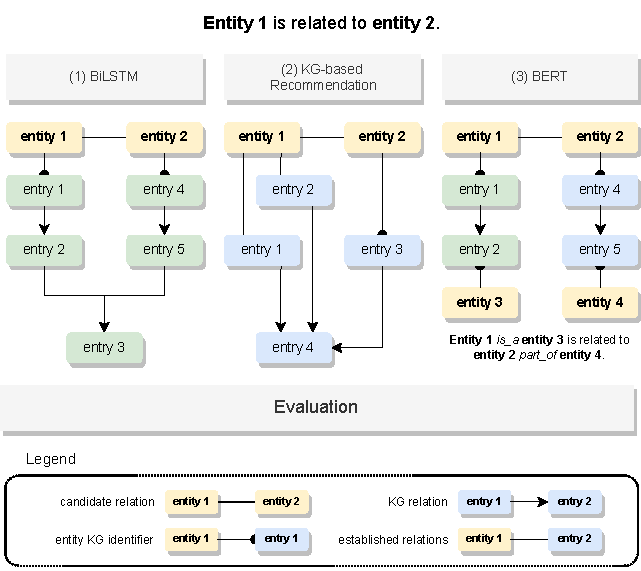
\includegraphics[width=\linewidth]{images/chapter_1/general_metodology.pdf}
\caption[Overview of the General Methodology]{Overview of the methodology followed to accomplish each defined objective. (1) BiLSTMs are a type of RNN composed of multiple layers, which can include entity annotation layers. These annotation layers link each entity to its ontology identifier. In the example, \textit{entity 1} corresponds to \textbf{entry 1} and \textit{entity 2} corresponds to \textbf{entry 4}. Then, we can go through the ontology until we find a common ancestor between the two entities (\textbf{entry 3}), reinforcing the candidate relation. (2) Knowledge Graph (KG)-based recommendation systems have shown the importance of external sources of knowledge to add additional features to items. In the example, knowing that there is a relation between \textit{entity 1} (user) and two other entities represented by \textbf{entry 1} and \textbf{entry 2} (items), that those items link to an \textbf{entry 4} in a KG and that \textit{entity 2} has the identifier \textbf{entry 3} that also links to \textbf{entry 4}, we can reinforce the candidate relation between \textit{entity 1} and \textit{entity 2}. (3) BERT is a language representation model that can be fine-tuned with just one additional output layer, making it possible to integrate the knowledge base data directly into the text where the candidate entities are mentioned. In the example, knowing that \textit{entity 1} has the identifier \textbf{entry 1} and \textit{entity 3} has the identifier \textbf{entry 2}, and that these identifiers are connected in a KG, we can directly integrate this knowledge in the text training data.} \label{fig1}
\end{figure}

\section{Contributions}

The main contributions of this thesis are the biomedical RE text mining solutions developed with added external biomedical knowledge and their evaluation through different approaches. The main chapters of this thesis consist of published articles written in the course of the doctoral work. All systems and datasets are available in open access through the links provided below. 

\subsection{Introductory Book Chapters}

Chapter 2 reflects the contents of two review articles regarding neural networks for relation extraction and text mining using biomedical literature.

\begin{itemize}
    \item{\textbf{Sousa, D.}, Lamurias, A., and Couto, F. M. (2021). \textbf{Using Neural Networks for Relation Extraction from Biomedical Literature}. In Artificial Neural Networks, pages 289–305. Springer, New York, NY, USA. (Q3 Scimago) \citep{sousa2021using}}
\end{itemize}

\begin{itemize}
    \item{Lamurias, A., \textbf{Sousa, D. F.}, and Couto, F. M. (2023). \textbf{Text Mining for Bioinformatics Using Biomedical Literature}. In Encyclopedia of Bioinformatics and Computational Biology. (Accepted) [\hyperlink{AB}{Appendix B}}] 
\end{itemize}

\subsection{Systems}

Chapters 3, 4, and 5 correspond to research articles that reflect the progression of the field of deep learning architectures throughout the doctoral work. Thus, each of the three articles describes a deep learning biomedical RE system, entitled BiOnt, K-BiOnt, and K-RET, respectively. BiOnt and K-RET bypassed the previous state-of-the-art by about 4\% and 3\% in average F-measure, respectively. While K-BiOnt retrieved more rare relations (i.e., complex to identify) than its predecessors. These systems correspond to Objective 1. 

\begin{itemize}
    \item{\textbf{Sousa, D.} and Couto, F. M. (2020). \textbf{BiOnt: Deep Learning Using Multiple Biomedical Ontologies for Relation Extraction}. In Advances in Information Retrieval: 42\textsuperscript{nd} European Conference on IR Research, pages 367–374, Lisbon, Portugal. Springer. (Core A) \citep{sousa2020biont}} \footnote{\url{https://github.com/lasigeBioTM/BiOnt}}
\end{itemize}

\begin{itemize}
    \item{\textbf{Sousa, D.} and Couto, F. M. (2022). \textbf{Biomedical Relation Extraction with Knowledge Graph-based Recommendations}. IEEE Journal of Biomedical and Health Informatics, 26(8):4207–4217. (Q1 Scimago) \citep{sousa2022biomedical}} \footnote{\url{https://github.com/lasigeBioTM/K-BiOnt}}
\end{itemize}

\begin{itemize}
    \item{\textbf{Sousa, D. F.} and Couto, F. M. (2023). \textbf{K-RET: Knowledgeable Biomedical Relation Extraction System}. Bioinformatics, 39(4):1-8. (Q1 Scimago) \citep{sousa2023k}} \footnote{\url{https://github.com/lasigeBioTM/K-RET}}
\end{itemize}

\subsection{Evaluation}

Chapter 6 corresponds to a research article that presents the usage of distant supervision techniques with crowdsourcing platforms to facilitate the creation of biomedical RE datasets. This work resulted in an average F-measure increase of about 35\% compared to relying solely on distant supervision when tested with two state-of-the-art systems. This approach corresponds to Objective 2. 

\begin{itemize}
    \item{\textbf{Sousa, D.}, Lamurias, A., and Couto, F. M. (2020). \textbf{A Hybrid Approach Toward Biomedical Relation Extraction Training Corpora: Combining Distant Supervision with Crowdsourcing}. Database, 2020:1-15. (Q1 Scimago) \citep{sousa2020hybrid}} \footnote{\url{https://github.com/lasigeBioTM/PGR-crowd}}
\end{itemize}

\subsection{Real-World Assessments}

Chapter 7 presents an overview of the work developed regarding workshops, challenges, and topic-adjacent journal contributions, such as participation in SemEval and BioCreative RE-specific community challenges. These contributions were deemed real-world assessments of the systems and approaches developed in this thesis, all corresponding to at least one of the two objectives in some capacity. 

\begin{itemize}
    \item{\textbf{Sousa, D.}, Lamurias, A., and Couto, F. M. (2020). \textbf{Improving Accessibility and Distinction Between Negative Results in Biomedical Relation Extraction}. Genomics \& Informatics, 18(2):1-4. \citep{sousa2020improving}} \footnote{\url{https://github.com/lasigeBioTM/blah6}}
\end{itemize}

\begin{itemize}
    \item{Lamurias, A., \textbf{Sousa, D.}, and Couto, F. M. (2020). \textbf{Generating Biomedical Question Answering Corpora From Q\&A Forums}. IEEE Access, 8:161042–161051. (Q1 Scimago) \citep{lamurias2020generating}} \footnote{\url{https://github.com/lasigeBioTM/BiQA}}
\end{itemize}

\begin{itemize}
    \item{Barros, M., Lamurias, A., \textbf{Sousa, D.}, Ruas, P., and Couto, F. M. (2020). \textbf{COVID-19: A Semantic-Based Pipeline for Recommending Biomedical Entities}. In Proceedings of the 1\textsuperscript{st} Workshop on NLP for COVID-19 (Part 2) at EMNLP 2020, pages 1–9, Online. Association for Computational Linguistics. (Core A) \citep{barros2020covid}} \footnote{\url{https://github.com/lasigeBioTM/knowledge-extraction-from-CORD-19}}
\end{itemize}

\begin{itemize}
    \item{\textbf{Sousa, D.}, Cassanheira, R., and Couto, F. M. (2021). \textbf{lasigeBioTM at BioCreative VII Track 1: Text Mining Drug and Chemical-Protein Interactions Using Biomedical Ontologies}. In Proceedings of the BioCreative VII Challenge Evaluation Workshop, pages 1–4, Online. Association for Computational Linguistics. \citep{sousalasigebiotm}} \footnote{\url{https://github.com/lasigeBioTM/biocreativeVII}}
\end{itemize}

\begin{itemize}
    \item{\textbf{Sousa, D.} (2021). \textbf{Deep Learning System for Biomedical Relation Extraction Combining External Sources of Knowledge}. In Advances in Information Retrieval: 43\textsuperscript{rd} European Conference on IR Research, pages 688–693, Berlin, Heidelberg. Springer. (Core A) \citep{sousa2021deep}}
\end{itemize}

\begin{itemize}
    \item{Barros, M.\footnote[*]{Authors contributed equally to this research}, Ruas, P.\textsuperscript{*}, \textbf{Sousa, D.}\textsuperscript{*}, Bangash, A. H., and Couto, F. M. (2021). \textbf{COVID-19 Recommender System Based on an Annotated Multilingual Corpus}. Genomics \& Informatics, 19(3):1-7. \citep{barros2021covid}} \footnote{\url{https://github.com/lasigeBioTM/blah7}}
\end{itemize} 

\begin{itemize}
    \item{Conceição S. I. R., \textbf{Sousa, D. F.}, Silvestre, P. M., and Couto, F. M. (2023). \textbf{lasigeBioTM at SemEval-2023 Task 7: Improving Natural Language Inference Baseline Systems with Domain Ontologies}. (Accepted)} \footnote{\url{https://github.com/lasigeBioTM/SemEval2023_Task-7}}
\end{itemize}

\begin{itemize}
    \item{Ruas, P.\footnote[†]{Authors contributed equally to this research}, \textbf{Sousa, D. F.}\textsuperscript{†}, Neves, A.\textsuperscript{†}, Cruz, C., and Couto, F. M. (2023). \textbf{LASIGE and UNICAGE Solution to the NASA LitCoin NLP Competition}. (Submitted) (7\textsuperscript{th} Place in the NASA LitCoin NLP Challenge with cash prize of 5.000 USD)} \footnote{\url{https://github.com/lasigeBioTM/Litcoin-Lasige_Unicage}}
\end{itemize}

\section{Document Structure}

In addition to the present introductory chapter, this document is structured into eight chapters as follows:

\begin{itemize}
   \item \textbf{Chapter \hyperlink{2}{2}} (Biomedical Relation Extraction) provides an overview of the key concepts to understand biomedical RE according to the two main objectives established previously. 
   \item \textbf{Chapter \hyperlink{3}{3}} (BiOnt: Deep Learning Using Multiple Biomedical Ontologies for Relation Extraction) presents the BiOnt system, a BiLSTM-based system with annotation layers based on biomedical ontologies. 
   \item \textbf{Chapter \hyperlink{4}{4}} (Biomedical Relation Extraction with Knowledge Graph-based Recommendations) showcases the K-BiOnt system. This system joins the abilities of KG-based recommendation systems and BiOnt by defining biomedical entities as items and ontological KG annotations as features. 
   \item \textbf{Chapter \hyperlink{5}{5}} (K-RET: Knowledgeable Biomedical Relation Extraction System) presents the K-RET system, a BERT-based system with added biomedical knowledge in the form of text expansion in the fine-tuning stage. 
   \item \textbf{Chapter \hyperlink{6}{6}} (A Hybrid Approach toward Biomedical Relation Extraction Training Corpora: Combining Distant Supervision with Crowdsourcing) demonstrates how to combine distant supervision approaches with crowdsourcing to boost the creation of biomedical RE datasets. 
   \item \textbf{Chapter \hyperlink{7}{7}} (Real-World Assessments) compiles all other research work conducted throughout this thesis by dividing each contribution into a section summarising its motivation and the work developed. 
   \item \textbf{Chapter \hyperlink{8}{8}} (General Discussion and Conclusions) closes the thesis by presenting a general discussion of the thesis, its main conclusions, and future work.
\end{itemize}

\hypertarget{2}{}

\rhead{Biomedical Relation Extraction}
\lhead{Chapter 2}

\chapter[Biomedical Relation Extraction]
{\huge Biomedical Relation Extraction}

\vspace{-1.6cm}

% Gray Line
\begingroup
\color{black}
\par\noindent\rule{\textwidth}{0.4pt}
\endgroup

\noindent{This chapter provides an overview of the key concepts to understand biomedical Relation Extraction (RE) according to the two main objectives established in Chapter \hyperlink{1}{1}. It also presents some of the approaches for RE by order of complexity and the methods/steps needed for their evaluation. The chapter corresponds to a combination of two review articles as mentioned in the introductory chapter: \hyperlink{AA}{Appendix A} \citep{sousa2021using} and \hyperlink{AB}{Appendix B}.}

\section{Learning for Relation Extraction}

Using different sources of information to support the automated extraction of relations between biomedical concepts contributes to the development of our understanding of biological systems. Researchers have proposed several RE approaches to identify relations between concepts in biomedical literature, namely, using neural network algorithms. The possibility of using multichannel architectures composed of multiple data representations, as in deep neural networks, leads to state-of-the-art results. The right combination of data representations can eventually lead us to even higher evaluation scores in RE tasks. The following sections will present the baseline concepts that are the building blocks for RE, the initial approaches to performing RE, and the different approaches, systems, and evaluation practices for deep learning RE.  

\hypertarget{2.1.1}{\subsection{Natural Language Processing}}

Natural Language Processing (NLP) is a field in computer science that aspires to obtain meaning from highly heterogeneous or unstructured text written by humans. This field covers several techniques that constitute pre-processing steps for the tasks described in the following section. NLP techniques target different goals and are often combined to obtain higher performance:

\begin{itemize}
    \item \textbf{Tokenization} breaks the text into tokens to be processed individually or as a sequence. The tokens are usually words but can also be phrases, numbers, and other types of elements. The most straightforward form of tokenization is breaking the input text by whitespaces or punctuation. However, with literature that is descriptive and formal, we have to account for complex entities. These entities tend to be morphologically complex and need specialized tokenization pipelines. Some researchers use a compression algorithm \citep{sennrich2015neural}, byte pair encoding (BPE), to account for vocabulary variability. BPE represents open vocabularies through a fixed-size vocabulary of variable-length character sequences, making it suitable for neural network models, for instance.

    \item \textbf{Stemming and Lemmatization} reduces the variability of natural language by normalizing a token to its base form (stem) \citep{manning2008introduction}. Also, it can take into account the context of the token, along with vocabulary and morphological analysis, to establish the canonical form of the word (lemma). The lemma is always a real word, but the stem can correspond only to a fragment of a word. For example, the stem of the word \textit{having} is \textit{hav}, and the lemma is \textit{have}.

    \item \textbf{Part-of-Speech (POS) Tagging} assigns each word of a sentence to the category where it belongs, taking into account its context (e.g., adverb or preposition). Each word can belong to one or more categories. This feature expresses the role of a word in a given sentence. 

    \item \textbf{Parse Tree} represents the syntactic structure of a sentence. There are two types of parse trees: constituency-based parse trees and dependency-based parse trees. The main difference between the two is the distinction between the terminal and non-terminal nodes. The first makes that distinction, and in the second, all nodes are terminal. In constituency-based parse trees, each node of the tree is either a \textit{branch} node, a \textit{leaf} node, or a \textit{root} node. For each sentence, there is only one \textit{root} node. The \textit{leaf} node is terminal, and the \textit{branch} node connects to two or more \textit{child} nodes. These leaves correspond to the lexical tokens \citep{aho1986compilers}. Dependency-based parse trees are usually simpler because they only identify the primary syntactic structure, leading to fewer nodes. The structures created by parse trees are used as inputs for other algorithms and can be constructed based on supervised learning techniques.
\end{itemize}

\hypertarget{2.1.2}{\subsection{Text Mining Primary Tasks}}

Text mining is a widespread approach to identifying and extracting information from unstructured or highly heterogeneous text \citep{westergaard2018comprehensive}. Text mining is used to extract facts and relationships in a structured form that can be used to annotate specialized databases and transfer knowledge between domains \citep{fleuren2015application}. Text mining can be considered as a sub-field of data mining. Thus, with the transformation of text into appropriate data representations, we can apply data mining algorithms, namely numeric vectors. In recent years, text mining tools have evolved remarkably in quality and number, but there are still several challenges in applying text mining to scientific literature. The main challenges are the heterogeneity and complexity of the written resources, making the retrieval of relevant information (i.e., relations between entities) a non-trivial task. 

Text Mining tools can target different tasks separately or together. Some primary tasks are detailed below, including RE. 

\begin{itemize}
    \item \textbf{Topic Modelling:} the classification of documents according to their topics or themes. This task aims to organize a set of documents to identify which documents are more relevant to a given topic \citep{blei2012probabilistic}. Related tasks include document triage \citep{buchanan2007investigating} and document clustering.

    \item \textbf{Named Entity Recognition (NER):} consists of identifying entities that are mentioned in the text. In most cases, the exact location of each entity in the text is required, given by the offset (position) of its first and last characters. In some cases, discontinuous entities may be considered, requiring multiple offset pairs. The classification of entity properties such as its type (e.g., protein, cell line, chemical) can be included in this task \citep{nadeau2007survey}.

    \item \textbf{Normalization:} consists of matching each entity to an identifier belonging to a knowledge base that unequivocally represents its  concept. For example, a protein may be mentioned by its full name or an acronym; in this case, the normalization process should assign the same identifier to both occurrences. The identifiers can be provided by an external database or ontology \citep{tsuruoka2008normalizing}. Similar tasks include named entity disambiguation \citep{bunescu2006using}, named entity linking (NEL), and harmonization.

    \item \textbf{Relation Extraction (RE):} the identification of entities that participate in a relationship described in the text. Most tools consider relations between two entities in the same sentence, but some focus on $n$-ary relations (between more than two entities) across multiple sentences \citep{singhal2016text}. Biomedical relations commonly extracted are gene-phenotype and drug-drug interactions \citep{segura2014lessons}.

    \item \textbf{Event Extraction:} can be considered an extension of the RE task, where the label of the relation and role of each participant is specified. The events extracted should represent the mechanisms described in the text \citep{Ananiadou2010}. Related tasks include slot-filling and relation classification.

    \item \textbf{Question Answering (QA):} is a task where we aim to automatically answer questions asked by humans in natural language using either an existing structured database or a collection of natural language documents \citep{CALIJORNESOARES2020635}.
\end{itemize}

\subsection{Initial Approaches}

Through the years, RE approaches became increasingly more intricate with the associated growth in performance. This section describes the RE approaches and some of their applications that preceded the deep learning-based RE systems. Due to the inherent complexity of highly heterogeneous or unstructured literature, initial approaches for RE worked on a sentence level \citep{lamurias2017extracting} and focused primarily on binary relations \citep{zhang2017review}.

\subsubsection{Co-occurrence}

Co-occurrence assumes that if two entities are mentioned in the same sentence (co-occur), they are likely related. Usually, this approach's application results in a higher recall (most entities co-occurring in a sentence participate in a relation) and lower precision. 
Some methods use frequency-based scoring schemes to eliminate relations identified by chance \citep{zweigenbaum2007frontiers}. Nowadays, applications occasionally use co-occurrence as a baseline against more complex approaches \citep{bunescu2006integrating}. 

\hypertarget{2.1.3.2}{\subsubsection{Pattern-based}}

Pattern-based uses manually defined patterns and automatically generated patterns to extract relations.

\textbf{Manually defined patterns} require domain expertise knowledge about the type of entities, their interactions, and the subject. 
Initial systems made use of regular expressions to match word patterns that reflected a relation between two entities \citep{smolinski2009computational}, making use of a dictionary of words that express relation, such as \textit{trigger} and \textit{stimulate}. Later systems introduce POS tagging, but this has proven to be too naive, mainly when applied to complex sentences, such as the ones that we typically find in scientific literature \citep{hao2005discovering}. Opposite to the co-occurrence approaches, manually defined patterns frequently achieve high precision but tend to have a poor recall. This approach does not generalize well and therefore is difficult to apply to new unseen data. 

\textbf{Automatically generated patterns} encompass two main approaches, bootstrapping with seeds \citep{wang2011inference} and leveraging of the corpora \citep{liu2011graphs}. 
The bootstrapping method uses a small set of relations known as seeds (e.g., person-occupation pairs). The first step is to identify the seeds in the dataset and map the relation pattern they describe. The second step is to try to apply the mapped patterns to the dataset to identify new pairs of relations that follow the same construction. Finally, the original set of relations is expanded by adding these new pairs. When, after repeating all previous steps, no more pairs are found, the process ends. Some systems apply distant supervision techniques to keep track of the validity of the added patterns. Distant supervision uses existing knowledge base entries as gold standards to confirm or discard a relation \citep{jiang2018revisiting}. This method is susceptible to noisy patterns as the original set of relations grows.
On the other hand, the leveraging of the corpora method makes immediate use of the entire dataset to generate the patterns. This method requires a higher number of annotated relations and produces highly specific patterns that cannot match new unseen data. Automatically generated patterns can achieve higher recall than manually defined patterns, but overall the noisy patterns continue to damage the precision. Nevertheless, there were a few efforts to reduce the number of noisy patterns \citep{nguyen2010simple}. 

\subsubsection{Rule-based}

Rule-based also uses manually defined and automatically generated rules from the training data to extract relations. Depending on the systems, the differences between pattern-based and rule-based approaches can be minor. 
Ruled-based approaches use not only patterns but also additional restraints to cover issues that are difficult to express by patterns, such as checking for the negation of the relations \citep{koike2005automatic}. Some ruled-based systems distance themselves from pattern-based approaches by replacing regular expressions with heuristic algorithms and sets of procedures \citep{rinaldi2007mining}. Like pattern-based approaches, ruled-based approaches tend to have a poor recall, even though rules tend to be more flexible. The trade-off recall/precision can be improved using automatic methods for rule creation \citep{xu2012feature}.

\subsubsection{Machine Learning (ML)}

Accordingly to the types of corpora, researchers divide RE based on machine learning into three domains \citep{zhang2017review}: supervised learning methods, semi-supervised learning methods, and unsupervised learning methods, beyond the deep learning methods described in Section \hyperlink{2.1.4}{2.1.4}. 

\textbf{Supervised machine learning} uses large annotated corpora to perform RE. These corpora are pre-processed using NLP tools and then used to train classification models. It is possible to categorize these ML methods into two main approaches, Feature-based and Kernel-based. \textbf{Feature-based approaches} represent each instance (e.g., a sentence) as a vector in an $n$-dimensional space. Support Vector Machines (SVM) classifiers tend to be used to solve binary classification problems and are considered black boxes because it can be difficult to interpret and understand the underlying decision-making process. These classifiers can use different features that are meant to represent the data characteristics (e.g., shortest path, bag-of-words (BOW), and POS tagging) \citep{kim2008detection}. \textbf{Kernel-based approaches} main idea is to quantify the similarity between the different instances in a dataset by computing the similarities of their representations \citep{giuliano2006exploiting}. Kernel-based approaches add the structural representation of instances (e.g., by using parse trees). These methods can use one kernel or a combination of kernels (e.g., graph, sub-tree (ST), and shallow linguistic (SL)). SVM classifiers do not need to use kernels. However, kernels are commonly used in these classifiers to the point where their use is subtended by most users. 

\textbf{Semi-supervised or weekly supervised learning} methods mainly encompass the bootstrap method described previously (Section \hyperlink{2.1.3.2}{2.1.3.2}) \citep{hoffmann2011knowledge,augenstein2015extracting}. It is mostly used in the field of knowledge extraction to solve classification and RE problems. 
This learning method reduces the dependence on human participation and corpus annotation. However, the bootstrap method has the problem of semantic drift when in the iterative process, damaging the RE's performance.

Supervised and semi-supervised learning methods need to determine the type of relation in advance. Large-scale corpora implies multiple relations, and most of the time, those methods are not able to grasp all of that variety. 

\textbf{Unsupervised learning} was first used to grasp a more varied pool of relations based on clustering \citep{hasegawa2004discovering,shinyama2006preemptive}. 
The idea was to use text information clustering between two entities to express the relation class. This formulation was successfully applied to multiple approaches and improved to multilevel clustering by \cite{shinyama2006preemptive}. In unsupervised learning, some researchers also developed methods based on pattern clustering (i.e., Density-based methods) and sentence parsing \citep{quan2014unsupervised}. 
This category of methods makes it hard to describe the relation name accurately and has difficulties catching low-frequency relations (i.e., leading to low recall).


\hypertarget{2.1.4}{\subsection{Deep Learning}}

Artificial neural networks are a parallel combination of small processing units (nodes) which can acquire knowledge from the environment through a learning process and store the knowledge in the connections between the nodes \citep{haykin1994neural} (represented by direct graphs \citep{guresen2011definition}). The process is inspired by the biological brain function, having each node corresponding to a \textit{neuron} and the connections between the nodes representing the \textit{synapses}. Artificial neural networks use fully connected layers to connect every neuron in one layer to every neuron in another layer. 
The first application of neural networks to NLP was language modelling, which has been useful in learning distributed representations (embeddings) for words \citep{bengio2003neural,mikolov2013distributed}. These data representations (i.e., word embeddings) were the initial step for a new way to successfully perform several NLP tasks based on neural networks \citep{nguyen2015relation}.  


\subsubsection{Convolutional Neural Networks (CNN)}

Some deep learning RE systems use Convolutional Neural Networks (CNN) to further encode the sentences, capturing $n$-gram level features. CNN consists of three parts: the input layer; the output layer; and several hidden layers, including convolutional layers, pooling layers, fully connected layers, and normalization layers \citep{xue2018relation}. 
In the convolutional layers, a convolution operation reduces the number of free parameters in the following way. Given an input sentence $x$ as a sequence of vectors $x = \{w_1,w_2,...,w_m\},\ w_i \in \mathbb{R}^d$, where $w_i$ represents the words in the $x$ sentence,  $m$ is the size of the input sentence, and $d$ is the dimensionality of the embedding space. If we have $l$ as the window size for the convolutional layer kernel, then the vector for the $i$-th window is formed by concatenating the input vectors for that window:

\begin{equation}
    q_i = w_{i:i+l-1};\ (1 \leq i \leq m-l+1);\ q_i \in \mathbb{R}^{(d \times l)}
\end{equation}

Then, a single convolutional kernel could be represented by a weight vector $W$ and a bias $b$, and the output for the $i$-th window computed as:

\begin{equation}
    p_i= f (W'q_i+b)
\end{equation}

where $f$ is the activation function. The shape of the output of the convolutional kernel $p$ would be $p \in \mathbb{R} ^{(m-l+1)}$. If the convolutional layer was a set of $d_c$ convolutional kernels, the output of the layer would be of the shape $\mathbb{R} ^{d_c \times (m-l+1)}$.
The convolutional operation allows the network to be more in-depth with fewer parameters, passing the result to the pooling layers. These layers (and also convolutional layers) provide a fixed-size output matrix and reduce the output dimensionality while keeping the essential information. 

\hypertarget{2.1.4.2}{\subsubsection{Recurrent Neural Networks (RNN)}}

Recurrent Neural Networks (RNN) are artificial neural networks where the nodes' connections follow a contrary path to the data flux. Thus, RNNs can use their internal state, or \textit{memory}, to process each input sequence. 
%RNNs, like some deep learning techniques, aim to train classification models based on word embeddings, POS tagging, and other features. 
RNN classifiers have multilayer architectures, where each layer learns a different representation of the input data. This characteristic makes RNN classifiers flexible to multiple text mining tasks without requiring task-specific feature engineering. Hence, while training, RNN keeps remembering the context, and each state can be defined by:

\begin{equation}
    h_t = f(h_{t-1}, x_t)
\end{equation}

where $x_t$ refers to the input and $h_t$ symbolizes the output, at a given time ($t$). Then, to each state we apply an activation function:

\begin{equation}
    h_t = tanh(W_{hh} \times h_{t-1} + W_{hx} \times x_t)
\end{equation}

where $W$ is the weight, $h$ is the single hidden vector, $W_{hh}$ is the weight at the previous hidden state, $W_{hx}$ is the weight at the current input state, and $tanh$ is an activation function that implements a non-linearity that squashes the activations to the range $[-1,1]$. Then, the output state is:

\begin{equation}
    y_t = W_{hy} \times h_{t}
\end{equation}

where $W_{hy}$ is the weight at the output state.

\paragraph{Long Short-Term Memory Networks (LSTMs)}

Long Short-Term Memory (LSTM) networks are an alternative to regular RNN \citep{hochreiter1997long}. LSTMs are a type of RNN that handles long dependencies (e.g., sentences), making this classifier more suitable for scientific domains, for instance, where sentences are usually long and descriptive. LSTMs solve the vanishing problem of RNN using back-propagation, and its main constituents are three gates (the input gate, the output gate, and the forget gate).
In recent years, using LSTMs to perform RE tasks became widespread in various domains, such as semantic relations between nominals \citep{miwa2016end}. \textbf{Bidirectional LSTMs} use two LSTM layers at each step, one that reads the sentence from right to left, and other that reads from left to right. The combined output of both layers produces a final score for each step. Bidirectional LSTMs have yielded better results than traditional LSTMs when applied to the same datasets \citep{zhang2015bidirectional}.

\subsubsection{Transformers}

Transformers were first introduced in 2017 \citep{vaswani2017attention}, greatly improving the performance of many NLP tasks, including RE. Transformers' performance is based on their ability to capture long-range dependencies and process sequential data, such as sentences or time-series data, with a robust attention mechanism. The transformer architecture is based on two components: the encoder and the decoder. The encoder takes an input sequence and processes it in parallel to create a sequence of hidden representations, capturing the contextual information of each input token. The decoder, on the other hand, takes the encoder's output and generates an output sequence autoregressively, one token at a time, attending to the encoder's representations. BERT \citep{devlin2019bert}, GPT \citep{radford2018improving}, and T5 \citep{raffel2020exploring} are transformers-based systems that nowadays have become the foundation systems for most NLP approaches.

\hypertarget{2.1.4.4}{\subsubsection{Data Representations}}

The combination of multiple and different languages and entity-related data representations is vital for the success of neural network models dedicated to RE tasks. Some of these features were already described in Section \hyperlink{2.1.1}{2.1.1}, such as POS tagging and parse trees:

\begin{itemize}
    \item \textbf{Shortest Dependency Path} (SDP) is a feature that identifies the words between two entities mentioned in the text, concentrating the most relevant information while decreasing noise \citep{xu2015classifying}. 
    \item \textbf{WordNet Hypernyms} are a feature that helps to hierarchize entities, structuring words similar to direct acyclic graphs \citep{miller1998wordnet}. For example, a \textit{vegetable} is a hypernym of \textit{tubers}, which in turn constitutes a hyponym of \textit{vegetable}. This feature is comparable to an ontology in the sense that a hierarchy relation is identified but misses the identification of relations between the different terms.
    \item \textbf{Word Embeddings} are fixed-sized numerical vectors that aim to capture the syntactic and semantic word relationships. These word vector models use multiple different pre-training sources. For instance, Word2Vec \citep{mikolov2013distributed} uses English Wikipedia, and BERT \citep{devlin2019bert} uses both English Wikipedia and BooksCorpus. 
    Early models, such as Word2Vec, learned one representation per word, but this proved to be problematic due to polysemous and homonymous words. Recently, most systems started to apply one embedding per word sense. One of the reasons why BERT outperforms previous methods is because it uses contextual models, meaning that it generates a unique representation for each word in a sentence. For instance, in the sentence fragments, \textit{couple got \textbf{engaged}}, and \textit{students were very \textbf{engaged} in}, the word \textit{engaged} for non-contextual models would have the same meaning. BERT also outperforms other word vector models that take into account the sentence context, such as ELMo \citep{peters2018deep} and ULMFit \citep{howard2018universal}, due to being an unsupervised and deeply bidirectional pre-trained language representation.
\end{itemize}

Using different features as information sources feeding individual channels like those mentioned above leads to multichannel architecture models. Multichannel approaches were proven effective in RE tasks \citep{xu2015classifying}. 

Regarding biomedical RE, LSTMs were successful in identifying drug-drug interactions \citep{wang2017dependency}, gene-mutation relations \citep{song2018n}, and drug-mutation relations \citep{peng2017cross}, among others. The BR-LSTM \citep{xu2018leveraging} model uses a multichannel approach with pre-trained medical concept embeddings. Using the Unified Medical Language System (UMLS) concepts, BR-LSTM applies a medical concept embedding method developed by \cite{de2014medical}. BO-LSTM \citep{lamurias2019bo} uses the relations provided by domain-specific ontologies to aid the identification and classification of relations between biomedical entities in biomedical literature. Some methods use domain-specific biomedical resources to train features for biomedical tasks. BioBERT \citep{lee2020biobert} is a domain-specific language representation model pre-trained on large-scale biomedical corpora, based on BERT \citep{devlin2019bert} architecture, similar to PubMedBERT \citep{gu2021domain}, and SciBERT \citep{scibert}. BioBERT, using minimal task-specific architecture modifications, significantly outperforms previous biomedical state-of-the-art models in the text mining primary tasks of NER, Normalization, and RE. 

\section{External Knowledge for Relation Extraction}

Semantic resources such as knowledge bases and graphs can contain highly structured background data, particularly for the biomedical domain \citep{li2020bio}. These resources play a fundamental role in the way we store, organize and retrieve information. More specifically, biological knowledge bases are commonplace for researchers and clinicians to access all types of biomedical data retrieved from biomedical literature \citep{arnaboldi2020text}. These resources can be explored by researchers regarding information retrieval systems, so one can rely on more than the literature itself to train a RE model. By integrating semantic resources, we feed the training process with extra, highly relevant information about each entity in the relation and the connections that that entity establishes within the known semantic universe.

\subsection{Knowledge Graphs}

Different perspectives or taxonomies \citep{lee2019attention} can classify graph-structured data. One of those taxonomies that focus on problem setting regarding the type of input relevant for RE is whether the graph is homogeneous or heterogeneous. A homogeneous graph is a graph where all the edges and nodes are of the same type. In contrast, heterogeneous graphs have a set of node types and a set of edge types. A bipartite graph is a simple heterogeneous graph with two node types and a single edge type. Figure \ref{figure:graphs} represents the three types of graphs: \ref{figure:a} homogeneous, \ref{figure:b} heterogeneous, and \ref{figure:c} bipartite graph. 

\begin{figure}[h]
\captionsetup{font=small}
\centering
\begin{subfigure}[b]{0.3\textwidth}
    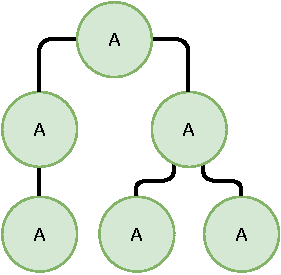
\includegraphics[width=4.5cm]{images/chapter_2/graph_a.pdf}
    \caption{}
    \label{figure:a}
  \end{subfigure}
  \begin{subfigure}[b]{0.3\textwidth}
    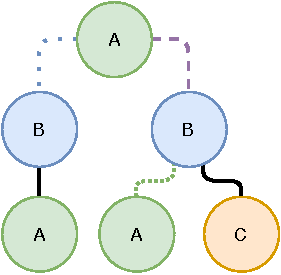
\includegraphics[width=4.5cm]{images/chapter_2/graph_b.pdf}
    \caption{}
    \label{figure:b}
  \end{subfigure}
  \begin{subfigure}[b]{0.3\textwidth}
    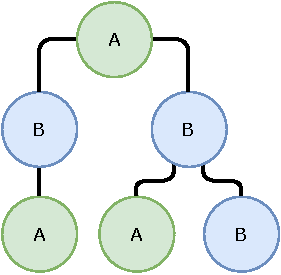
\includegraphics[width=4.5cm]{images/chapter_2/graph_c.pdf}
    \caption{}
    \label{figure:c}
  \end{subfigure}
\fontsize{9}{10.8}\caption[Types of Graphs According to Input]{Three types of graphs, according to the type of input: \textbf{(a)} homogeneous, \textbf{(b)} heterogeneous, and \textbf{(c)} bipartite graph.}
\label{figure:graphs}
\end{figure}

In the last few years, some works have emerged regarding heterogeneous graph attention mechanisms. \cite{zhou2019hahe} proposed a Hierarchical Attentive Heterogeneous information network Embedding (HAHE) model that takes into account personalized preferences of different nodes on different meta paths in each semantic space. Similarly, in the biomedical domain, \cite{hosseini2019hierarchical} introduced a target-aware hierarchical attention mechanism for diagnosis prediction using Electronic Health Records (EHR). Also, \cite{yang2020interpretable} tries to bridge the shortcomings of previous systems, regarding flexibility in exploiting all possible meta-paths and scalability, by proposing an interpretable and efficient Heterogeneous Graph Convolutional Network (ie-HGCN) to learn representations of nodes. 

Using heterogeneous graphs attention mechanisms to represent indirect relations between different type entities, such as genes and diseases in the biomedical domain, can be a viable additional external source of knowledge to preexisting deep learning RE systems \citep{wu2020comprehensive}. Thus, enabling us to find representations of an indirect relation between two entities using knowledge graphs. The candidate knowledge graphs to implement heterogeneous graphs attention mechanisms could be ontologies representing the entities of interest and their semantic relationships in a given domain. \cite{li2020bio} took an attention mechanism approach to identify protein-protein interactions, using attention mechanisms within a Bidirectional Long-Short Term Memory neural network (BiLSTM). Their attention mechanism leads on the knowledge base (KB) information from BioModels\footnote{\url{https://www.ebi.ac.uk/biomodels/}} and filters the information with the weight vector to reflect how external information is relevant to the current state $h_t$ (Section \hyperlink{2.1.4.2}{2.1.4.2}). However, they struggle with KB coverage and how to efficiently integrate external information and do not use heterogeneous graph attention mechanisms, which could be of great value for information retrieval from biomedical literature. 

According to \cite{ehrlinger2016towards}, the difference between a knowledge graph and an ontology could be interpreted either as a matter of quantity (e.g., a large ontology) or of extended requirements (e.g., a built-in reasoner that allows new knowledge to be derived). However, the consensus is that ontologies are smaller collections of hand-curated assertions, usually for solving a domain-specific problem, upping their reliability. 

\subsubsection{Ontologies}

An ontology is a structured way of providing a common vocabulary in which shared knowledge is represented \citep{gruber1993translation}. Word embeddings can learn how to detect relations between entities but manifest difficulties in grasping the semantics of each entity and its specific domain. Domain-specific ontologies provide and formalize this knowledge. Biomedical ontologies are usually structured as a directed acyclic graph, where each node corresponds to an entity, and the edges correspond to known relations between those entities. Thus, a structured representation of the semantics between entities and their relations, an ontology, allows us to use it as an added feature to a machine learning classifier. Some of the biomedical entities structured in publicly available ontologies are genes properties/attributes (Gene Ontology (GO) \citep{ashburner2000gene}), phenotypes (Human Phenotype Ontology (HPO) \citep{robinson2010human}), diseases (Human Disease Ontology (DO) \citep{schriml2012disease}), and chemicals (Chemical Entities of Biological Interest (ChEBI) \citep{hastings2016chebi}). All of these entities participate in relations with different and same domain-type entities. Hence, the information about each entity on a semantic level adds a new layer of knowledge to increase the performance of RE classifiers. 

Non-biomedical models using ontologies as an added source of information to neural networks are becoming widespread for several tasks. \cite{li2016learning} propose using word sense definitions provided by the WordNet ontology to learn one embedding per word sense for word sense disambiguation tasks. \cite{ma2017ontology} focus their work on semantic relations between ontologies and documents, using the DBpedia ontology. Some researchers explored graph embedding techniques \citep{goyal2018graph} that convert relations to a low dimensional space which represents the structure and properties of the graph. Other researchers have combined different sources of information, including ontological information, to do multi-label classification \citep{kong2013multi} and used ontology concepts to represent word tokens \citep{dasigi2017ontology}.

However, few authors have used biomedical ontologies to perform RE. Textpresso \citep{muller2004textpresso} is a text-mining system that works as a search engine for individual sentences acquired from the full text of scientific articles and articles. It integrates biomedical ontological information (e.g., of genes, phenotypes, and proteins), allowing for article and sentence search a query by term. The integration of ontological information allows for semantic queries. This system helps database curation by automatically extracting biomedical relations. The IICE \citep{lamurias2014identifying} system uses kernel-based support vector machines and an ensemble classifier to identify and classify drug-drug interactions, linking each chemical compound to the ChEBI ontology. \cite{tripodi2017knowledge} system focuses on drug-gene/protein interaction discovery to aid database curation using ChEBI and GO ontologies. BO-LSTM \citep{lamurias2019bo} incorporates ancestry information from biomedical ontologies with deep learning to extract relations from the text, such as drug-drug interactions and gene-phenotype relations. 

\section{Evaluation for Relation Extraction}

The evaluation of deep learning systems is done by applying the trained models to a test set. Gold standard test sets are manually curated or annotated by domain experts and unseen by the system. For a binary sentence-based RE task, the test set should correspond to the list of pairs of entities (e.g., person-organization or gene-disease pairs) that co-occur in the same sentences and their relation.

\subsection{Results}

For any given information extraction system, it is necessary to define what constitutes a positive and negative result, particularly in the biomedical domain. Researchers and clinicians need to have access not only to known relations between biomedical entities but also to relations that were already disproven. Accessible negative results limit their search space and prevent the costly re-exploration of research hypotheses. However, most biomedical RE datasets do not seek to distinguish between a false and a negative relation between two biomedical entities, and few knowledge bases hold negative examples. Some domain-specific exceptions are worth noticing, such as the Negatome database \citep{blohm2014negatome} for protein-protein interactions and the phenotype-disease relations annotation file made available by the Human Phenotype Ontology (HPO) organization \citep{robinson2010human} that contains both positive and negative relations.

A false relation should express a context where the entities are not related. In contrast, a negative relation should explicitly express a context where there is an affirmation of no association between the two entities. Furthermore, datasets created using distant supervision techniques also have some false negative relations that constitute undocumented/unknown relations \citep{sousa2019silver}. These relations are not marked true because they are not described in a knowledge base at the moment of the dataset creation, even though upon reading the context of these relations within their respective sentences, one can support a true relation. Unknown relations are good examples of hypotheses to be further explored by researchers and clinicians and can be of use to effectively populate the biomedical relations knowledge bases. In RE tasks, the binary type of results possible are Relation that can be either positive or negative, and No Relation that is only false, shown in Table \ref{table:evaluation}.

\begin{table}[ht]
\centering
\caption[Types of Results Obtained with an Information Extraction System for a Relation Extraction Task]{Types of results obtained with an information extraction system for a RE task}
\begin{tabular}{ccc}
\hline
Annotator (Gold Standard) & System & Classification\\
\hline
\multirow{2}{*}{Relation} & Relation & True Positive (TP) \\
 & No Relation & False Negative (FN) \\ 
\hline
\multirow{2}{*}{No Relation} & Relation & False Positive (FP) \\
 & No Relation & True Negative (TN) \\
 \hline
\end{tabular}
\label{table:evaluation}
\end{table}

\subsection{Metrics}

The primary goal of a given information retrieval system is to maximize the number of TP and TN. To compare results obtained with different datasets or different tools, we have three distinct evaluation metrics: recall, precision, and F-measure. Precision represents how often the results are correct, recall the number of correct results identified, and F-measure is a combination of both metrics to express overall performance, being the harmonic mean of precision and recall:

\begin{equation}
F-measure = \frac{2\times Precision\times Recall}{Precision + Recall} = \frac{2 TP}{2 TP + FP + FN}
\label{equation:evaluation}
\end{equation} 

Occasionally, Accuracy is also used to consider the number of TNs and expresses the overall correctness of a classification model. It represents the proportion of correctly classified instances (or predictions) of a dataset's total number of instances.

Some approaches also consider the Area under the precision-recall curve (AUPRC) to measure the trade-off between precision and recall at various thresholds. It comprehensively evaluates a model's performance across different operating points and is particularly useful when dealing with imbalanced datasets. Also, the Area under the receiver operating characteristic curve (AUROC) measures the trade-off between true positive rate (TPR or recall) and false positive rate (FPR) at various classification thresholds. While commonly used in binary classification tasks, it may not be the most suitable metric for biomedical relation extraction due to class imbalance issues.

Additionally, depending on the specific application and requirements, other metrics such as specificity, sensitivity, and the Matthews correlation coefficient (MCC) may be used to evaluate the performance of biomedical relation extraction models. 

Also, it is important to note that statistical significance testing and p-values can be relevant in specific research scenarios in biomedical relation extraction, where they are used to validate the significance of associations or correlations between variables or features. 

\subsection{Datasets}

There are three types of datasets for RE. The first type is the \textbf{traditional information extraction datasets}, where relations are manually annotated and pre-determined. Some examples of these types of biomedical datasets:

\begin{itemize}
    \item \textbf{AImed} \citep{mooney2006subsequence} describes interactions between human proteins (e.g, \textit{sigma(K)} interacts with \textit{cwlH}). It consists of 225 Medline abstracts, of which 200 describe interactions, with around 1000 tagged interactions.
    \item \textbf{BioNLP Shared Task} \citep{kim2011overview} describes relations between proteins and components, and sub-units and complexes (e.g., \textit{fimV} regulates \textit{FimS}). The corpus consists of 1210 Medline abstracts with 2834 relations. 
    \item \textbf{ADE-V2} \citep{gurulingappa2012development} describes relations between drugs and drug-related adverse effects (e.g., \textit{ticlopidine} causes \textit{severe aplastic anemia}). It consists of 2872 PubMed documents describing 7100 relations. 
    \item \textbf{DDI} \citep{herrero2013ddi} describes interactions between pharmacological substances/drugs (e.g., \textit{perindoprilat} effects \textit{diuretics}). The corpus consists of 792 texts selected from the DrugBank database and 233 Medline abstracts and describes 34449 relations. 
    \item \textbf{BC5CDR} \citep{li2016biocreative} describes relations between chemicals and diseases (e.g., \textit{timolol} effects \textit{myocardial infarction}). The corpus consists of 1500 PubMed articles with 3116 chemical-disease interactions.
    \item \textbf{BioRED} \citep{luo2022biored} describes relations pairs between genes/proteins, diseases, and chemicals (e.g., \textit{D374Y} positively correlates to \textit{autosomal dominant hypercholesterolemia}). It consists of 600 PubMed abstracts with 6503 relations. 
\end{itemize}

The second type is \textbf{open information extraction datasets}, where relations are manually annotated but can be of any type \citep{fader2011identifying,del2013clausie,mesquita2013effectiveness}. 

Finally, the third type is \textbf{distantly supervised datasets}, where distant supervision is applied, and the relations are usually pre-determined. This last type has been rapidly expanding for being less costly and time-consuming than the previous \citep{riedel2010modeling}. One example of these datasets in the biomedical domain is the PGR Corpus \citep{sousa2019silver} that describes relations between human phenotypes and genes and precedes the work developed in this thesis.

\section{Current Challenges} 

Biomedical RE has its domain-specific challenges to overcome, such as sentence and entity complexity, lack of models for languages other than English, lack of standardization of nomenclature for biomedical entities such as human phenotypes and diseases, and lack of datasets to train models (in English and other languages). 

To tackle sentence and entity complexity, we have some preprocessing tools that aim to mask the information deemed unnecessary for RE \citep{miwa2010entity,lee2020biobert}. Thus, instead of contemplating the whole region between the target pair, this region is simplified by giving different weights to each element in the sentence or even removing unnecessary words that are not relation-related. The use of word embeddings explicitly trained for the biomedical domain has shown to be effective for all biomedical NLP-related tasks \citep{lee2020biobert,scibert}.

Biomedical RE targeting non-English literature is essential due to the sheer quantity of biomedical research written in other languages (approximately 16\% just in PubMed\footnote{as of January 2022}). For instance, clinical reports are almost always written in the medical practitioner/patient native language \citep{10.1093/database/bax064}. This literature holds relevant information that can be of interest to support or discard a scientific hypothesis \citep{nussbaumer2020excluding}, and it is rarely considered \citep{di2017publish}. Some works target biomedical RE in non-English languages \citep{6103454}. At the same time, other researchers are dedicated to the translation of biomedical resources such as ontologies like the Human Phenotype Ontology to other languages such as Spanish and Portuguese\footnote{\url{https://github.com/drseb/HPO-translations}}. 

The lack of standardization of nomenclature for biomedical entities is prominent since biomedical NLP first emerged \citep{leser2005makes,horwitz2011naming}. Although this problem can seem to be a NER problem, since NER is a necessary precedent step to RE, it also affects RE, particularly with entities that use more than one word. The multi-word entities, such as the disease \textit{breast cancer}, come with some challenges. The first is if we consider more than one level relation by dividing multi-word entities, for instance, \textit{breast cancer} and the gene \textit{BRACA1} and \textit{cancer} and the gene \textit{BRACA1}. The second challenge is if we can imply the two relations even if the KB supporting the gold standard relations only considers the gene \textit{BRACA1} having a relation with \textit{cancer} and not \textit{breast cancer}, for instance. In some examples, it is easy for us to consider relation transfer, but for others, it is more challenging. It is not trivial to formulate a rule that fits all cases for all the different biomedical entities. 

Finally, the fourth challenge for the biomedical RE task is the lack of annotated datasets to train models. One solution can be creating these datasets through distant supervision allied with crowdsourcing, although it still brings some concerns, such as reliability and bias depending on the platform and pre-defined settings.  

The following four chapters tackle the absence of structured, high-quality knowledge integrated into RE systems (Chapters 3, 4, and 5) and the need for gold standard corpora to validate those systems (Chapter 6). Chapter 7 assesses the work done throughout the thesis by applying it to multiple community-driven workshops and challenges, among other applications.  



\hypertarget{3}{}

\rhead{BiOnt: Deep Learning Using Multiple Biomedical Ontologies for Relation Extraction}
\lhead{Chapter 3}

\chapter[BiOnt: Deep Learning Using Multiple Biomedical Ontologies for Relation Extraction]
{\huge BiOnt: Deep Learning Using Multiple Biomedical Ontologies for Relation Extraction \\
\Large \textmd{Diana Sousa and Francisco M. Couto}}

\vspace{-1.6cm}

% Gray Line
\begingroup
\color{black}
\par\noindent\rule{\textwidth}{0.4pt}
\endgroup

\noindent{This chapter tackles Objective 1 by showcasing the integration of biomedical ontologies into a BiLSTM \acl{RE} (RE) model and corresponds to the conference paper:} 

\begin{itemize}[label=]
    \item{\textbf{Sousa, D.} and Couto, F. M. (2020). \textbf{BiOnt: Deep Learning Using Multiple Biomedical Ontologies for Relation Extraction}. In Advances in Information Retrieval: 42\textsuperscript{nd} European Conference on IR Research, pages 367–374, Lisbon, Portugal. Springer. (Core A) \citep{sousa2020biont}} 
\end{itemize}

\textbf{Abstract.} Successful biomedical relation extraction can provide evidence to researchers and clinicians about possible unknown associations between biomedical entities, advancing the current knowledge we have about those entities and their inherent mechanisms. Most biomedical relation extraction systems do not resort to external sources of knowledge, such as domain-specific ontologies. However, using deep learning methods, along with biomedical ontologies, has been recently shown to effectively advance the biomedical relation extraction field. To perform relation extraction, our deep learning system, BiOnt, employs four types of biomedical ontologies, namely, the \acl{GO} (GO), the \acl{HPO} (HPO), the \acl{DO} (DO), and the \acl{ChEBI} (ChEBI), regarding gene products, phenotypes, diseases, and chemical compounds, respectively. We tested our system with three datasets that represent three different types of relations of biomedical entities. BiOnt achieved, in F-measure, an improvement of 4.93 percentage points for drug-drug interactions (\acs{DDI} Corpus), 4.99 percentage points for phenotype-gene relations (\acs{PGR} Corpus), and 2.21 percentage points for chemical-induced disease relations (\acs{BC5CDR} Corpus), relatively to the state-of-the-art. The code supporting this system is available at \url{https://github.com/lasigeBioTM/BiOnt}.

\section{Introduction}

The description of the mechanisms that are responsible for the behaviour of biological systems is non-trivial, and each step towards the understanding of those mechanisms often constitutes a scientific achievement \citep{YU2006252,BECHTEL2007269}. Typical examples describe diseases that are associated with mechanisms that originate phenotypic abnormalities as a result of modified gene expression, as well as the action of drugs on those diseases \citep{Campaner2011}, among others. One significant step to fully understanding biological systems mechanisms is to extract and classify the relations that exist between the different biomedical entities, namely chemicals, diseases, genes, and phenotypes. In literature, authors classify this problem as a \acl{RE} (RE) task. Biomedical \ac{RE} aims to extract and classify relations between biomedical entities in highly heterogeneous or unstructured scientific or clinical text.

Deep learning is widely used to solve problems such as speech recognition, visual object recognition, and object detection. Lately, deep learning based-systems have started to tackle \ac{RE} problems. These systems are becoming increasingly more complex, namely the MIMLCNN \citep{jiang2016relation} and PCNN + Att \citep{lin2016neural} systems, that mark recent turning points in the deep learning \ac{RE} field. Both of these systems use Word2Vec \citep{mikolov2013distributed} that aims to capture the syntactic and semantic information about the word \citep{kumar2017survey}. However, deep learning methods that effectively extract and classify relations between biomedical entities in the text are still scarce \citep{li2017neural,lamurias2019bo}. 

Ontologies play an important role in biomedical research through a variety of applications and are used primarily as a source of vocabulary for standardization and integration purposes \citep{Bodenreider08biomedicalontologies}. Word embeddings can learn how to detect relations between entities but manifest difficulties in grasping the semantics of each entity and its specific domain. Domain-specific ontologies provide and formalize this knowledge. Thus, a structured representation of the semantics between entities and their relations, an ontology, allows us to use it as an added feature to a machine learning classifier. Some of the biomedical entities structured in publicly available ontologies are genes properties/attributes (\ac{GO}) (45003 terms) \citep{ashburner2000gene,gene2019gene}, phenotypes (\ac{HPO}) (25810 terms) \citep{kohler2017human}, diseases (\ac{DO}) (18114 terms) \citep{10.1093/nar/gky1032}, and drugs/chemicals (\ac{ChEBI}) (133104 terms) \citep{hastings2016chebi}\footnote{term counts at \textit{09/09/2019}}.  

This work presents the BiOnt system, a biomedical \ac{RE} system built using bidirectional \acl{LSTM} (LSTM) networks. The BiOnt system incorporates the state-of-the-art Word2Vec word embeddings \citep{mikolov2013distributed} and makes use of different combinations of input channels to maximize performance. Our system is based on the work of \cite{lamurias2019bo} and \cite{xu2018leveraging}. Both of these models make use of biomedical resources as embedding layers for their respective systems. \cite{lamurias2019bo} uses the \cite{xu2018leveraging} model as a baseline with an added ontological embedding layer (BO-LSTM model). However, the BO-LSTM model is limited to two types of relations, namely, drug-drug and gene-phenotype relations.

External sources of knowledge, such as biomedical ontologies, can provide highly valuable information for the detection of relations between entities in the text, as described previously by \cite{lamurias2019bo}. These knowledge bases provide not only relevant characteristics about the respective entities but also about the underlying semantics of the relations they establish. This information is not expressed directly in the training data but usually reinforces a relation between two entities in the text. The novelty of our system is that it expands the previous work done by \cite{lamurias2019bo} by using four types of domain-specific ontologies and combines them to extract new types of relations, along with word embeddings \citep{mikolov2013distributed} and WordNet hypernyms \citep{ciaramita2006broad}. BiOnt successfully replicates the results of the BO-LSTM application using different types of ontologies. Our system can extract new relations between four biomedical entities, namely, genes, phenotypes, diseases, and chemicals. Figure \ref{fig31} shows how these four types of biomedical ontologies can be combined to aid the relation extraction of ten different combinations of biomedical entities. The BiOnt system also explores the use of entities that are not direct entries in an ontology (e.g., genes), linking each entity to its most informative annotation concept within a corresponding ontology (e.g., GO). Our method incorporates more ontologies than the previously mentioned systems and is evaluated using three state-of-the-art datasets. The BiOnt system can be used to effectively populate knowledge bases regarding gold standard relations. Ultimately, it can be used to explore new experimental hypotheses providing evidence to researchers and clinicians about possible unknown associations between biomedical entities.

\begin{figure}[h]
\centering
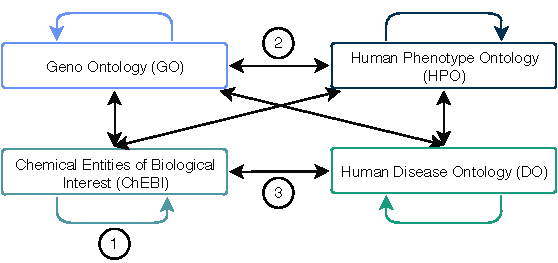
\includegraphics[width=0.8\linewidth]{images/chapter_3/ecir_2020_1.pdf}
\caption[Ten Possible Combinations Between Four Biomedical Ontologies]{The ten possible combinations between the four biomedical ontologies (\ac{GO} \citep{ashburner2000gene}, \ac{HPO} \citep{kohler2017human}, \ac{DO} \citep{10.1093/nar/gky1032}, and \ac{ChEBI} \citep{hastings2016chebi}). The \textbf{1} represents the \acs{DDI} Corpus, the \textbf{2} the \acs{PGR} Corpus, and the \textbf{3} the \acs{BC5CDR} Corpus (described in Section 3).} \label{fig31}
\end{figure}


\section{Methodology}

This section describes the BiOnt model with an emphasis on the enhancements done to the BO-LSTM \cite{lamurias2019bo} model to allow multi-ontology integration, expanding the number of different type candidate pairs from two to ten. The BiOnt model uses a combination of different language and entity-related data representations that feed individual channels creating a multichannel architecture. The input data is used to generate instances to be classified by the model. Each instance corresponds to a candidate pair of entities in a sentence. To each instance, the model assigns a positive or negative class. A positive class corresponds to an identified relation between two biomedical concepts, where the nature of this relation depends on the dataset being used to perform the evaluation, and a negative class implies no relation between the different entities. 

An instance should condense all relevant information to classify a candidate pair. To create an instance, the BiOnt model relies on three primary data information layers. After sentence tokenization, these layers are Shortest Dependency Path (SDP) \citep{Pyysalo:2013b,mikolov2013distributed}, WordNet Classes \citep{ciaramita2006broad}, and Ontology Embeddings. The latter represents the relations between the ancestors for each ontology concept corresponding to an entity (Figure \ref{fig6}). The model assumes that the input data already has the offsets of the relevant entities identified and their respective concept ID, the Named-Entity Recognition and Linking tasks. However, while most entities already correspond to an ontology concept ID, some entities, such as genes, do not have a direct entry into an ontology. BiOnt matches these entities to their most representative concept in the \acl{GO} \citep{ashburner2000gene}. To match the gene to their most representative GO term, the priority was given to concepts inferred from experiments, for having a more sustained background and usually being more descriptive. For tie-breaking, if we have several GO terms inferred from experiments, the choice is the term that is the most specific (i.e., with the longer ancestry line).

\begin{figure}[h]
\centering
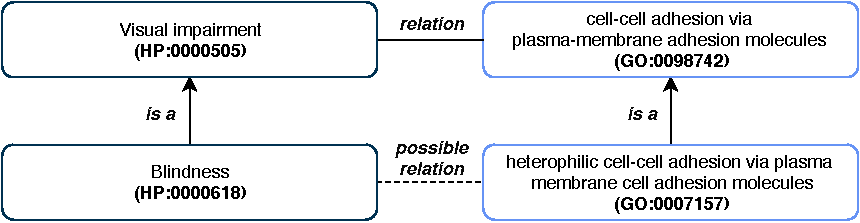
\includegraphics[width=\linewidth]{images/chapter_3/ecir_2020_6.pdf}
\caption[BiOnt Ontology Embedding Illustration]{BiOnt ontology embedding illustration based on the HPO and the GO ontologies, for the candidate relation between the human phenotype \textit{blindness} and the gene \textit{CRB1} (represented by the GO term \textit{heterophilic cell-cell adhesion via plasma membrane cell adhesion molecules}).} \label{fig6}
\end{figure}

As stated previously, our system expands the work done by \cite{lamurias2019bo} by using four types of domain-specific ontologies and combining them to extract new types of relations. Therefore, to allow this diversity of relations, we adapted the BO-LSTM model common ancestors and the concatenation of ancestors channels. Since the common ancestors' channel could only be used for relations between the same type of biomedical entities, we only use the concatenation of the ancestors' channel for the relations between different biomedical entities. 


\section{Evaluation}

To showcase our systems' performance, we used three different state-of-the-art datasets. These  represent three out of the ten possible combinations of the biomedical entities used in this work, drug-drug interactions, phenotype-gene relations, and chemical-induced disease relations. With these datasets, we intend to show the flexibility of our model to the different types of biomedical entities represented by biomedical ontologies. Figure \ref{fig31} illustrates how the entities present in the three  (\textbf{1}, \textbf{2}, and \textbf{3}) are connected to the different biomedical entities.

Drug-Drug Interactions (1) The SemEval 2013: Task 9 DDI Extraction Corpus \citep{herrero2013ddi} is a corpus that describes drug-drug interactions (DDIs) focused on both pharmacokinetic (PK) and pharmacodynamic (PD) DDIs. The manually annotated corpus created by \cite{herrero2013ddi} combines 5028 DDIs, from selected texts of the DrugBank database and  Medline abstracts. 

Phenotype-Gene Relations (2) The Phenotype-Gene Relations Corpus (PGR) \citep{sousa2019silver} is a corpus that describes human phenotype-gene relations, created in a fully automated manner. Due to being a silver standard corpus is not expected to be as reliable as manually annotated corpora. Nonetheless, the authors show the system's efficiency by training two state-of-the-art relation extraction deep learning systems. The PGR corpus combines 4283 human phenotype-gene relations.

Chemical-Induced Disease Relations (3) The BioCreative V CDR Corpus (BC5CDR) \citep{li2016biocreative} is a corpus of chemical-induced disease (CID) relations. The BC5CDR corpus consists of 3116 chemical-disease interactions annotated from PubMed articles. To use the BC5CDR corpus, we had to preprocess the documents linking the annotations of the relations to their sentences. We assumed that if two entities share a relation in the document, they will continue to share that relation if present in the same sentence of that document. 

\section{Results and Discussion}

Table \ref{tab32} presents the relation extraction results of our system, BiOnt, for each dataset. For all three datasets, our system performs better using the ontological embeddings layer (+ Ontologies) than just using the word embeddings and WordNet classes layers (State-of-the-art) by an average of 0.0404. The most relevant contribution for this metric was an increase in recall for the DDI and PGR corpora and in precision for the BC5CDR corpus. The ontology embeddings contribute to the identification of more correct relations, with a small trade-off in precision, for the DDI corpus. For the other two datasets, the ontological embedding layer does not damage the precision, while more correct relations are identified.

\begin{table}[h]
\centering
\caption[Relation Extraction Results with the BiOnt System]{Relation extraction results with the BiOnt system, for each dataset, expressing drug-drug interactions (DDI Corpus), phenotype-gene relations (PGR Corpus), and chemical-induced disease relations (BC5CDR Corpus)}\label{tab32}
\begin{tabular}{llccc}\hline
Dataset & Configuration & Precision & Recall & F-measure \\
\hline
\multirow{2}{*}{DDI Corpus} & State-of-the-art & 0.7134 & 0.6410 & 0.6753 \\
&  + Ontologies & 0.6784 & 0.7775 & \textbf{0.7246} \\
\hline
\multirow{2}{*}{PGR Corpus} & State-of-the-art & 0.8421 & 0.6666 & 0.7442 \\
& + Ontologies & 0.8438 & 0.7500 & \textbf{0.7941} \\
\hline
\multirow{2}{*}{BC5CDR Corpus} & State-of-the-art & 0.5371 & 0.7264 & 0.6175 \\
& + Ontologies & 0.5770 & 0.7173 & \textbf{0.6396} \\
\hline
\end{tabular}
\end{table}


For the DDI corpus, the BiOnt system, due to the inherent variability of the preprocessing phase (by randomizing the division between training and test sets), when compared with the BO-LSTM system, performed slightly worse (0.7246 in F-measure) than the previously reported results (0.7290 in F-measure).
The paper supporting the PGR corpus \citep{sousa2019silver} reported some deep learning applications results, including with the BERT \citep{devlin2019bert} based BioBERT \citep{lee2020biobert} pre-trained biomedical language representation model (0.6716 in F-measure). Our system outperformed those results with an F-measure of 0.7941.
Regarding the BC5CDR corpus, our system outperformed the best system (0.5703 in F-measure) in the challenging task chemical-induced disease (CID) relation extraction of BioCreative V, by 0.0693 \citep{inproceedingscdr}, with 0.6396 in F-measure. 
The differences in F-measure for the distinct datasets are mostly due to how they were built and the completeness and complexity of the respective ontologies. 
For instance, the PGR corpus is a silver standard corpus, therefore, could have entities that were poorly identified, not identified at all, or not linked to the right identifier. The BC5CDR corpus was annotated for documents, not regarding the offsets of the entities that shared a relation in each document, which is also a possible limitation.


\section{Conclusions and Future Work}

This work showed that the knowledge encoded in biomedical ontologies plays a vital part in the development of learning systems, providing semantic and ancestry information for entities such as genes, phenotypes, chemicals, and diseases. We evaluated BiOnt using three state-of-the-art datasets (DDI, PGR, and BC5CDR Corpora), obtaining improvements in F-measure (4.93, 4.99, and 2.21 percentage points, respectively) by using an ontological information layer. Our system successfully enhances the results of \cite{lamurias2019bo} to other entities and ontologies. BiOnt shows that integrating biomedical ontologies instead of relying solely on the training data for creating classification models will allow us not only to find relevant information for a particular problem quicker but possibly also to find unknown associations between biomedical entities.

Regarding future work, it is possible to integrate more ontological information in different ways. For instance, one could consider only the relations between the ancestors with the highest information content (more relevant for the candidate pair they characterize). The information content could be inferred from the probability of each term in each ontology or resorting to an external dataset. Also, a semantic similarity measurement could account for non-transitive relations (within the same ontology). Relatively to biomedical concepts that do not constitute ontology entries, we could explore quantitative evidence values, choose more than one representative term, and we could also employ semantic similarity measures \citep{COUTO2019870}.

\hypertarget{4}{}

\rhead{Biomedical Relation Extraction with Knowledge Graph-based Recommendations}
\lhead{Chapter 4}

\chapter[Biomedical Relation Extraction with Knowledge Graph-based Recommendations]
{\huge Biomedical Relation Extraction with Knowledge Graph-based Recommendations \\
\Large \textmd{Diana Sousa and Francisco M. Couto}}

\vspace{-1.6cm}

% Gray Line
\begingroup
\color{black}
\par\noindent\rule{\textwidth}{0.4pt}
\endgroup

\noindent{This chapter tackles Objective 1 by benefitting from the knowledge integration approaches in the \acl{KG} (KG) recommender systems field and developing a new method to perform biomedical \acl{RE} (RE). Corresponds to the journal article:} 

\begin{itemize}[label=]
    \item{\textbf{Sousa, D.} and Couto, F. M. (2022). \textbf{Biomedical Relation Extraction with Knowledge Graph-based Recommendations}. IEEE Journal of Biomedical and Health Informatics, 26(8):4207–4217. (Q1 Scimago) \citep{sousa2022biomedical}}
\end{itemize}

\textbf{Abstract.} Biomedical Relation Extraction (RE) systems identify and classify relations between biomedical entities to enhance our knowledge of biological and medical processes. Most state-of-the-art systems use deep learning approaches, mainly to target relations between entities of the same type, such as proteins or pharmacological substances. However, these systems are mostly restricted to what they directly identify on the text and ignore specialized domain knowledge bases, such as ontologies, that formalize and integrate biomedical information typically structured as direct acyclic graphs. On the other hand, \acl{KG} (KG)-based recommendation systems already showed the importance of integrating KGs to add additional features to items. Typical systems have users as people and items that can range from movies to books, which people saw or read and classified according to their satisfaction rate. This work proposes to integrate KGs into biomedical RE through a recommendation model to further improve their range of action. We developed a new RE system, named K-BiOnt, by integrating a baseline state-of-the-art deep biomedical RE system with an existing KG-based recommendation state-of-the-art system. Our results show that adding recommendations from KG-based recommendation improves the system's ability to identify true relations that the baseline deep RE model could not extract from the text. The code supporting this system is available at \url{https://github.com/lasigeBioTM/K-BiOnt}.


\section{Introduction}

The exponential growth in scientific literature does not allow researchers to keep up with all recent advances in their respective fields and in adjacent areas that could be of interest to their research \citep{10.1371/journal.pbio.2005343}. 
To this end, the field of \acl{NLP} (NLP) is mostly focused on automatic means to identify and extract relevant information from unstructured text \citep{indurkhya2010handbook, 9086146}. One of the prominent tasks of the NLP field is Relation Extraction (RE), which aims at extracting and classifying relations between entities of interest. Most Biomedical RE studies focus on extracting relations between the same and different types of entities, such as diseases, genes, phenotypes, and pharmacological substances. Recently, there have been several advances regarding this task, mostly using deep learning techniques \citep{8416973}. However, few make use of external sources of knowledge that are openly available such as domain-specific ontologies, which are highly popular in the biomedical domain. Using additional sources of knowledge can also result in more system explainability by facilitating the re-traceability of AI decisions to specific components of the models \citep{HOLZINGER202128}.

An ontology is a structured way of providing a common vocabulary in which shared knowledge is represented \citep{gruber1993translation}. Biomedical ontologies are usually structured as directed acyclic graphs. Each node corresponds to an entity, and the edges correspond to known relations between those entities of type \textit{is-a}. Some of the most prominent ever-evolving biomedical ontologies are the Gene Ontology (GO) \citep{gene2019gene}, the Chemical Entities of Biological Interest (ChEBI) \citep{hastings2012chebi}, the Disease Ontology (DO) \citep{schriml2012disease}, and the Human Phenotype Ontology (HPO) \citep{kohler2019expansion}. Yet, researchers do not incorporate this structured information in most biomedical RE deep learning models. 

On the other hand, Knowledge Graph (KG)-based Recommendation systems already showed the importance of external sources of knowledge to add additional features to items when using deep learning models \citep{10.1145/2827872,barros2019using,9216015}. This focus on external sources of knowledge could be highly relevant for the biomedical RE field since most researchers focus their work on already-known relations between biomedical entities, which implies that a large volume of relations is not explicitly described in the literature. Consequently, systems that rely solely on available literature to identify these relations do not have enough information to establish more complex interactions. Therefore, we need to go beyond the text and uncover how to integrate entity annotations knowledge into our systems, as in most recent recommendation systems. 

In this work, we propose to integrate a KG-based recommendation model into biomedical RE to answer the following question: \textit{Can recommendations add value to the biomedical RE task, enhancing their range of action?} 

\begin{figure*}[!h]
\centerline{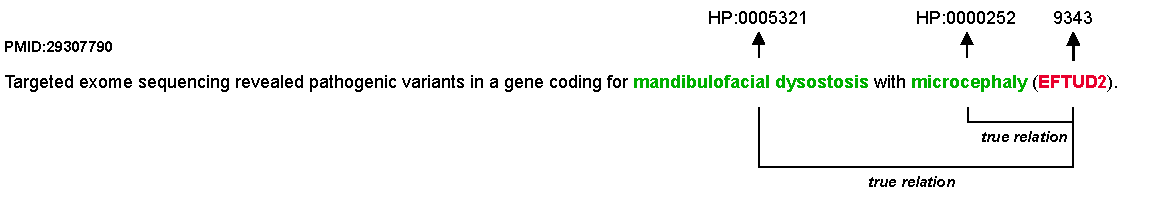
\includegraphics[width=\linewidth]{images/chapter_4/example_paper_knowledge_graph.pdf}}
\caption[Example of an Annotated Sentence]{An example of an annotated sentence retrieved from the PGR-crowd dataset from article PMID:29307790. The phenotype entities are linked to the HPO ontology (HP:0005321 and HP:0000252), and the gene entity is linked to the NCBI gene database (9343). We simplified the sentence to facilitate reading comprehension.}
\label{fig:example}
\end{figure*}

The first step towards biomedical RE based on recommendation was to adapt three publicly available RE datasets into the standardized recommender systems format of $<$user-item-rating$>$. We chose the PGR-crowd \citep{sousa2020hybrid} dataset that describes relations between human phenotypes and genes (Figure~\ref{fig:example}), the DDI Corpus \citep{herrero2013ddi}) that describes relations between drugs/chemicals, and the BC5CDR Corpus \citep{li2016biocreative}, that describes drugs/chemicals interactions with diseases, to demonstrate the range of our approach.

To make the adaption of biomedical RE datasets to the $<$user-item-rating$>$ recommendation format, we had first to decide which entities would be considered the users (\textit{user} entities) and the items (\textit{item} entities), for the datasets that had different type entities (PGR-crowd and BC5CDR dataset). Our choices for \textit{item} entities, described in detail in Section III under the A. Datasets sub-section, were to give priority to entities that were covered by ontological KGs (phenotypes in the PGR-crowd by the HPO) and to diversify the type of ontological KGs chosen (the DO for diseases in the BC5CDR Corpus). Therefore, as KGs, we used the ontologies HPO \citep{kohler2019expansion}, ChEBI \citep{hastings2012chebi}, and DO \citep{schriml2012disease}, linked to the \textit{item} entities when possible. 

Figure~\ref{fig:pipeline} illustrates an example of a relation recommendation where the user \textit{EFTUD2} is related to \textit{Microcephaly} and \textit{Mandibulofacial dysostosis} in our RE dataset of reference (Figure~\ref{fig:example}). Using the KG we can determine that one of the ancestor connections for \textit{Microcephaly} and \textit{Mandibulofacial dysostosis} is \textit{Abnormality of the skull}. By sharing an ancestor connection, these two items reinforce the connection between other descendants and the user \textit{EFTUD2}. Thus, we can recommend a relation between our user \textit{EFTUD2} and our item \textit{Cephalocele} (i.e., the green dashed line).

\begin{figure}[!h]
\centerline{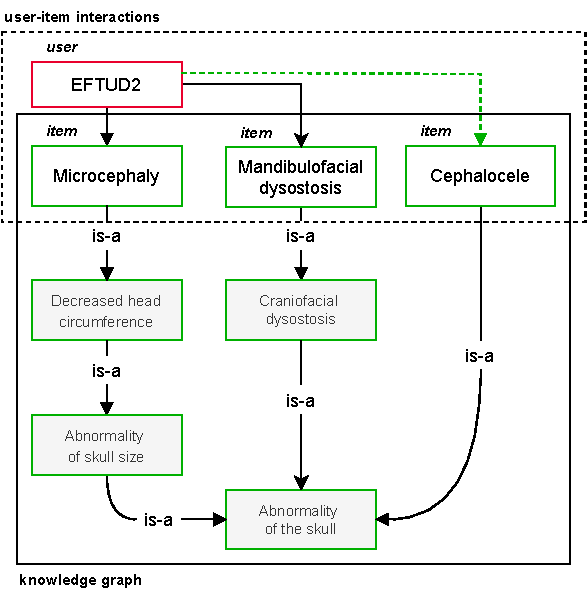
\includegraphics[width=0.6\textwidth]{images/chapter_4/paper_knowledge_graph.pdf}}
\caption[Example of a Relation Recommendation]{An example of a relation recommendation retrieved from the adapted PGR-crowd dataset \citep{sousa2020hybrid}. This example illustrates how a graph connection can contribute to a new relation recommendation.}
\label{fig:pipeline}
\end{figure}

In real-case scenarios, our approach would imply adapting existing and future RE biomedical datasets so that all entities are linked to a KG identifier, which by itself would enhance the applicability of such datasets. Moreover, linking identified entities to KGs is already a widely disseminated NLP task called Named-Entity Linking (NEL) or Concept/Entity Normalization, and most of the time, a natural precedent to RE \citep{huang2020biomedical}. As stated previously, a large volume of biomedical ontologies covers most types of studied entities. Therefore, the biggest hurdle would be to guarantee high KG coverage for the original datasets, while our adaptation of the datasets to a recommendation format is highly generalizable. For instance, given a biomedical sentence within a dataset, where the offsets of the entities of interest are identified and linked to KGs (Figure~\ref{fig:example}), the next step would be to give a rating to the possible relations considering the whole training dataset and identifying if there are other entities within the KG ancestry line that exhibit similar relations that can further support a true relation. Thus, we expect that the degree of coverage of each KG over each dataset dictates the effectiveness of the approach as well as other factors that we will discuss throughout this manuscript. 

After dataset re-formation, we adapted a state-of-the-art recommendation system to recommend relations between biomedical entities considering the specificities of the domain and evaluated the system's added value to a standard state-of-the-art deep learning biomedical RE system. 

In this paper, we present the results for relation recommendation on its own and then the added value of these recommendations to a deep learning biomedical RE system. Our results show that adding KG-based recommendations improves RE systems' ability to identify true relations in high KG coverage settings that baseline deep RE models could not extract from the text, indicating that the recommendation model adds value to the RE task. This work resulted in the following main contributions:

\begin{itemize}
    \item Pipeline for integrating a KG-based recommendation model in a biomedical RE system, including the adaptation of RE datasets for training. 
    \item Biomedical RE deep learning system with added knowledge in the form of KG-based recommendations (K-BiOnt).
\end{itemize}

The following section will present the related work for RE and recommender systems that specifically target the biomedical domain. We will then proceed to methodology, where we describe the dataset construction and the different training stages on their own and their joint evaluation. Next, we present results and discuss the effects of the KG-based recommendation on biomedical RE. Finally, we finish with the main conclusions and future work. 


\section{Related Work}

Biomedical RE is a task in NLP that usually follows Named-Entity Recognition (NER) and Named-Entity Linking (NEL) or Concept/Entity Normalization \citep{funk2014large}, the identification and mapping of entities in unstructured text, respectively \citep{sousa2021using}. This information extraction task mostly focuses on relations within the same sentence \citep{PMID:32032717}, with approaches that range from co-occurrence to a variety of Machine Learning methods. However, in recent years, deep learning approaches have become state-of-the-art for most domains achieving high levels of precision.
However, many biomedical relations are still hard to extract even when exploring the full documents \citep{verga-etal-2018-simultaneously}.
This can be explained by the complexity of the domain that requires extensive domain knowledge to be correctly perceived. 
One of those models, inspired by the BO-LSTM and BI-LSTM models \citep{lamurias2019bo,xu2018leveraging} is the BiOnt model \citep{sousa2020biont}. The BiOnt model uses deep learning methods along with domain-specific ontologies, achieving state-of-the-art results. Thus, it is a model that already explores external sources of knowledge to perform biomedical RE, even if with less KG depth than our proposal. Therefore, in this work, we propose a more in-depth use of KGs with recommendation approaches to detect missed true annotations by BiOnt, which we detail in the methodology section. We chose BiOnt over other biomedical or even non-biomedical \citep{devlin2019bert,gu2021domain} RE systems \citep{lee2020biobert} due to its use of similar external entity knowledge. If we can effectively improve the BiOnt model, it shows that their use of knowledge is not sufficient to fully grasp less frequent relations. Nevertheless, we also use the state-of-the-art BioBERT system \citep{lee2020biobert} on the same datasets to provide an extra comparison baseline. The BioBERT system is a BERT-based contextualized word representation model based on a masked language model and pre-trained using bidirectional transformers on large-scale biomedical corpora. 

Item recommendation initially focused on similarity-based methods that aimed at extracting features of users and items, computing their similarity, recommending similar users or items to a target user. Similarity-based methods using Neural Network (NN) models effectively extract latent features of users and items for recommendations \citep{10.1145/2959100.2959190,10.1145/3109859.3109872,huang2020efficient}. However, they deal with issues such as data sparsity \citep{guo2017resolving}, cold-start \citep{10.1145/3397271.3401426}, and lack of explainability \citep{10.1145/3397271.3401032} (i.e., an user understanding why an item is being recommended). Content-based methods introduce additional information, such as relational data \citep{10.1145/3309547} and knowledge graphs \citep{ai2018learning,10.1145/3308558.3313411}, and help relieve those issues. Therefore, recently, researchers have focused their attention on generating recommendations using knowledge graphs as additional information \citep{9216015,10.1145/3397271.3401428}, such as the TUP system created by \cite{10.1145/3308558.3313705}.

Current recommender systems that deal with biomedical data target different tasks, such as recommending ontologies to annotate biomedical text \citep{martinez2017ncbo}, model biological processes \citep{wang2020independent}, recommending drugs to target SARS-CoV-2 regarding the COVID-19 pandemic \citep{info:doi/10.2196/21169}, recommending entities of potential interest to specific researchers \citep{barros2019using}, or even recommending articles to expand existing biomedical datasets \citep{PATRA2020103399}. There is also a focus on recommending articles and venues to researchers to limit their search space \citep{PMID:30441232, info:doi/10.2196/12957}, for instance, by performing keyword-based recommendation \citep{yang2018keyword}. Further, there is a significant amount of work done on biomedical KG completion \citep{zhang2021drug,fei2020enriching,biswas2019relation}, including trying to depend less on domain-specific labelling and going through a minimum supervision route that can scale with the volume of literature available \citep{yuan2020constructing}. 


\section{Methodology}

To demonstrate the benefits of allying KG-based Recommendation to deep Biomedical RE, we used three publicly available datasets describing relations between different types of biomedical entities: the PGR-crowd \citep{sousa2020hybrid,sousa2019silver}, the DDI Corpus \citep{herrero2013ddi}, and the BC5CDR Corpus \citep{li2016biocreative}. The first step was to convert these RE datasets into a format compatible with KG-based Recommendation, which required several adjustments and rating assessments described in detail in the following section. Moreover, in this section, we will provide the training and evaluation details for each component system: deep biomedical RE and KG-based Recommendation on their own and as added features in a deep biomedical RE system plus recommendations. All baseline systems used or adapted throughout our work are openly available through their respective authors, including original configuration details.   

%here
\subsection{Datasets}

To take advantage of KG-based Recommendation into RE, we had to create standard $<$user-item-rating$>$ datasets using the PGR-crowd, DDI Corpus, and BC5CDR Corpus original RE datasets. These datasets describe relations between human phenotypes and genes, using NCBI gene database\footnote{\url{https://www.ncbi.nlm.nih.gov/gene}} and HPO identifiers (PGR-crowd), between drugs/chemicals, that can be linked to ChEBI ontology identifiers (DDI Corpus), and interactions between drugs/chemicals and diseases, that can be linked to the ChEBI and DO ontologies (BC5CDR Corpus). The PGR-crowd and DDI datasets are available in the same XML format, and the BC5CDR Corpus is available in a text format for standard RE applications. Table~\ref{tab:dl_statistics} presents the RE datasets' general statistics, including counts for the total number of entity annotations and the distribution of true and false relations. A relation is considered true if semantically there is an implication of an association between two entities considered in the same sentence, and false if there is no semantic relation or a semantic connection negates the relation between the entities. We did not consider the DDI Corpus relations' different label classifications for this work, only the binary classification of true/false. 

\begin{table}[h]
\centering
  \caption[Statistics of PGR-crowd, DDI Corpus, and BC5CDR Corpus Regarding Relation Extraction]{Statistics of PGR-crowd, DDI Corpus, and BC5CDR Corpus regarding Relation Extraction}
  \label{tab:dl_statistics}
  \begin{tabular}{lcccc}
    \hline
    \multirow{2}{*}{Dataset} & \multirow{2}{*}{Annotations} & \multicolumn{3}{c}{Relations} \\
    \cline{3-5}
    & & True & False & Total \\
    \hline
    PGR-crowd & 4150 & 5501 & 626 & 6127 \\
    DDI Corpus & 18491 & 5000 & 29449 & 34449 \\
    BC5CDR Corpus & 32527 & 1448 & 2294 & 3742 \\
    \hline
  \end{tabular}
\end{table}

Although the protocols were similar for the three datasets, we had to consider that in the PGR-crowd and BC5CDR datasets, each relation had two distinct entities (genes and human phenotypes, and drugs/chemicals and diseases, respectively). To cast our \textit{item} roles for the PGR dataset, we chose the phenotype entities since these were already mapped to an ontological knowledge graph (HPO). To diversify our approach, for the BC5CDR Corpus, we decided to map disease entities to the DO ontology as \textit{item} entities. While on the DDI Corpus dataset, we were dealing with relations between the same type of entities (i.e., drugs/chemicals) that could both be mapped to a knowledge graph (ChEBI). 

In the PGR-crowd dataset, we considered our \textit{users} as genes and our \textit{items} as human phenotypes. Each relation can appear more than once in a RE dataset since different sentences/articles can describe the same relation. We can have multiple instances of the same relation with the same or different labels. Therefore, we attributed $1$ to true relations and $-1$ to false relations and considered the rating the sum of all occurrences of the same relation within the training dataset. This process allowed us to have only one occurrence of each relation as expected in recommender systems type datasets, where the user only rates an item once. Figure~\ref{fig:datasets} further elucidates the process by direct comparison with an example of the MovieLens-1m dataset \citep{10.1145/2827872}. We followed the same procedure for the BC5CDR Corpus, where we considered our \textit{users} drugs/chemicals and our \textit{items} diseases.

\begin{figure}[!h]
\centerline{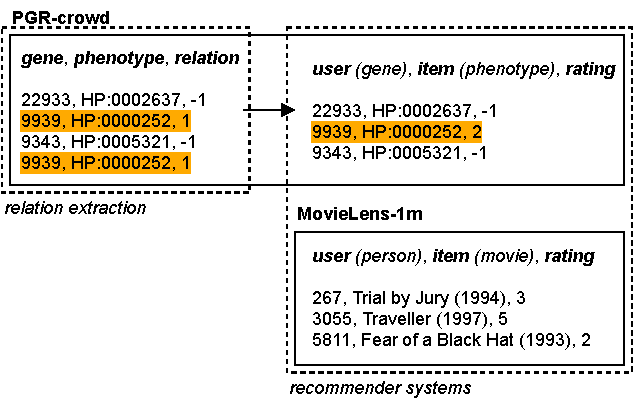
\includegraphics[width=0.6\textwidth]{images/chapter_4/datasets.pdf}}
\caption[Conversion from a Relation Extraction Type Dataset to a Recommender System Type Dataset]{The conversion from a relation extraction type dataset to a recommender system type dataset (PGR-crowd), including the comparison with examples from the MovieLens-1m dataset \citep{10.1145/2827872}.}
\label{fig:datasets}
\end{figure}

The DDI Corpus was not as straightforward to assign \textit{user} and \textit{item} roles to the drug/chemical entities. As each relation has two entities of the same type, we had to verify the symmetry between relations (e.g., is entity one an effect of entity two and vice-versa, or is it just a one-sided relationship?). For this, we considered the classification done by the creators of the DDI Corpus dataset, where each true relation could be of type \textit{effect} (asymmetric), \textit{mechanism} (asymmetric), \textit{advice} (symmetric), or \textit{int} (symmetric).  While the other types are intuitive, the \textit{int} type refers to the default positive interaction for which there is no additional information. So, we disregarded the entities' order for false and symmetric relations and maintained the order assigned for true asymmetric relations when adapting the RE dataset for recommendation. The process of calculating the ratings was identical to the previously described for the PGR-crowd and BC5CDR datasets. 

For model training, we converted all entities to an internal identifier. Also, the existing ratings were treated as positive interactions, while negative interactions were generated randomly by corrupting items following other models that target implicit feedback \citep{Wang_Wang_Xu_He_Cao_Chua_2019}. In the work done by \cite{10.1145/3308558.3313705}, the negative sampling was done by corrupting items that were less commonly used by users, which could not be applied to datasets with low average ratings. 

While previous works \citep{10.1145/2899005,bhargava2019collaborative} mapped publicly available datasets such as MovieLens-1m \citep{10.1145/2827872} and DBbook2014\footnote{\url{http://2014.eswc-conferences.org/important-dates/call-RecSys.html}} to DBPedia \citep{lehmann2015dbpedia} entities, whenever a mapping was available, we mapped our datasets to three publicly available biomedical ontologies (HPO for PGR-crowd, ChEBI for DDI Corpus, and DO for BC5CDR Corpus). For the PGR-crowd dataset, since the preexisting entity identifiers already linked to HPO, our coverage was 100\%. However, for the other two datasets (BC5CDR and DDI), the coverage was 26.0\% and 47.8\%, respectively, which is expected since the creators did not rely on the DO or ChEBI ontology to identify the original entities. The mapping was done automatically by exact matching, allowing for a Levenshtein distance of 1. Thus, particularly in the DDI and BC5CDR Corpora, we did not match possible synonym entities. Doing a more detailed mapping would require either the usage of external normalization tools \citep{funk2014large} or domain expertise to review all entities, which would be time and cost-intensive. However, we recognize the limitation in our entity normalization stage that could be improved in future work. In contrast with previous work \citep{10.1145/3308558.3313705}, we did not preprocess the datasets to filter low-frequency users and items or performed editing on the type of entities or relations in triples due to our universe being considerably smaller and the reassurance of using domain-specific ontologies instead of the generic domain of DBPedia. 

Table~\ref{tab:rs_statistics} describes the statistics for the three datasets (PGR-crowd, DDI Corpus, and BC5CDR Corpus) regarding the KG-based recommendation format. The data sparsity issue is prevalent in all datasets due to the low number of average ratings.

\begin{table}[h]
\centering
  \caption[Statistics of PGR-crowd, DDI Corpus, and BC5CDR Corpus Regarding Knowledge Graph-based Recommendation]{Statistics of PGR-crowd, DDI Corpus, and BC5CDR Corpus regarding Knowledge Graph-based Recommendation}
  \begin{tabular}{llccc}
    \hline
    && PGR-crowd & DDI Corpus & BC5CDR Corpus\\
    \hline
    \multirow{5}{*}{User-Item Interactions} & Users & 2176 & 2538 & 593 \\
    & Items & 409 & 2563 & 599 \\
    & Ratings & 4308 & 25973 & 2080 \\
    & Average Ratings & 2 & 10 & 4 \\
    & Sparsity & 99.5\% & 99.6\% & 99.4\% \\
    \hline
    \multirow{2}{*}{Knowledge Graph} & Entity & 15671 & 497046 & 13355 \\
    & Relation & 1 & 1 & 1 \\
    \hline
    \multirow{2}{*}{Multi-Tasks} & Item-Entity Alignments & 409 & 1225 & 156\\
    & Coverage & 100\% & 47.8\% & 26.0\%\\
    \hline
  \end{tabular}
  \label{tab:rs_statistics}
\end{table}

\subsection{Training}

The deep biomedical RE system BiOnt \citep{sousa2020biont} worked as our baseline since it achieved state-of-the-art performance in the datasets used in this work and also uses knowledge graphs as added information layers. We designed experiments regarding relation recommendation, following the work of \cite{10.1145/3308558.3313705}, and the incorporation of those recommendations into BiOnt (K-BiOnt). These systems were chosen due to their state-of-the-art results but also their availability and in-depth documentation. For all our experiments, we divided the datasets into a 6:1:3 ratio corresponding to the training set, the validation set, and the test set, respectively. We used the original datasets as provided for the Deep Learning component, making the appropriate parsing for the system specifications. While for the Recommendation component, we used the re-formatted datasets, as described in the previous sub-section. 


\subsubsection{Baseline Deep Learning Model}

The BiOnt model uses ontologies as external sources of knowledge to add information layers to a baseline deep learning model, following the work of \cite{lamurias2019bo}. An ontology is a formal definition of concepts related to a specific subject. It can be represented by a tuple $<C, R>$, where $C$ represents the set of concepts in an ontology and $R$ is the set of relations between the same ontology concepts. Similar to our dataset construction, the type of ontology relations considered by \cite{sousa2020biont} is subsumption relations, \textit{is-a} due to its transitive aspect. For instance, with $(c_1, c_2) \in R$, and $(c_2, c_3) \in R$, the authors assume that $(c_1, c_3)$ is a valid relation within the ontology. The ancestors of each concept $c$ are given by:

\begin{equation}
Anc(c) = a : (c, a) \in T
\label{equation:ancestors}
\end{equation}

where $T$ is the transitive closure of $R$. The authors define the common ancestors between the concepts $c_1$ and $c_2$ as:

\begin{equation}
CommRA(c_1, c_2) = Anc(c_1) \cap Anc(c_2)
\label{equation:commonancestors}
\end{equation}

A relation between different ontology concepts can be represented by $(x_1, y_1)$, where $x_1 \in X$ and $X$ represents the set of concepts in the first ontology and $y_1 \in Y$ and $Y$ represents the set of concepts in the second ontology. For instance, with $(x_2, y_2) \in RA$, where $RA$ is the set of relations between ancestors, and $(x_2\,\textit{is-a}\,x_1)$, and $(y_2\,\textit{is-a}\,y_1)$, their model assumes that $(x_1, y_1)$ is a valid relation. The concatenation of the relations between the ancestors of concepts $x_2$ and $y_2$ is defined using:

\begin{equation}
ConcRA(x_2, y_2) = Anc(x_2) \Join Anc(y_2)
\label{equation:cancestors}
\end{equation}

Since the common ancestors' channel could only be used for relations between the same type of biomedical entities (i.e., DDI Corpus), we only use the concatenation of ancestors channel for the relations between different biomedical entities (i.e., PGR-crowd). 

Each ontology concept corresponds to a one-hot vector $v_c$, a vector of zeros, except for the position corresponding to the concepts' ID. An embedding matrix $M \in \mathbb{R}^{D \times C}$ transforms these sparse vectors into dense vectors, where $D$ is the dimensionality of the embedding layer and $C$ is the number of concepts of the ontologies. Then, the output of the embedding layer is given by:

\begin{equation}
f(c) = M \cdot v_c
\label{equation:ontologyembedding}
\end{equation}

Next, the ontology embedding layer, with a dimensionality of 50 (as suggested by \cite{lamurias2019bo}), initializes its values randomly to be later tuned through back-propagation. Then, the vectors' sequence representing the relations between the ancestors of the terms is fed into a Long short-term memory (LSTM) layer, ordered from the more general concepts to the terms themselves. Finally, the system uses a max pool layer fed into a dense layer through a sigmoid activation function, and a softmax layer outputs the probability for each class.

The model was trained using a stochastic gradient descent optimization algorithm where weights were updated using the back-propagation of error algorithm. At each iteration, the model with a given set of weights creates predictions and computes the error for those predictions. The optimization algorithm seeks to alter the weights to reduce that error in the next evaluation. The relevant hyperparameters of this model tuned for our experiments were mini-batch gradient descent optimization algorithm (RMSprop), learning rate (0.0001), loss function (categorical cross-entropy), and dropout rate (0.500) for every layer except the penultimate and output layers.

We used the three standard evaluation metrics for RE models:
\textit{Precision}: Expresses how often the results are correct;
\textit{Recall}: It is the number of correct results identified;
\textit{F1 score}: Expresses overall performance by the harmonic mean of precision and recall.


\subsubsection{Item Recommendation} 

The TUP model created by \cite{10.1145/3308558.3313705} takes a list of user-item pairs $\mathcal{Y} = {(u, i)}$ as input, and outputs a relevance score $g(u, i; p)$, indicating the likelihood that $u$ likes $i$, given the preference $p \in \mathcal{P}$. In this work, instead of the terminology being \textit{the likelihood that $u$ likes $i$} is the likelihood that $u$ as a biomedical entity is related to $i$ as another biomedical entity. 
For each user-item pair, the TUP model induces a preference. The authors designed two strategies for preference induction: a hard approach that selects one out of the $P$ preferences and a soft way that combines all preferences with attentions. The soft strategy yielded a better performance for both authors' datasets. Therefore, we opted for this strategy to create our models. The preferences constitute the motives for each an \textit{user} entity may be connected to an \textit{item} entity. For traditional recommendation set-ups, these usually lack depth in explainability. To avoid that, in this work, we provided them explicit semantics by aligning them with the KG relations, capturing the intuition that the types of item attributes play a crucial role in user assignment. Considering that an entity might be related to another entity according to various factors, which can not be restricted by a firm boundary, instead of selecting the most prominent preference, the soft strategy combines multiple preferences via an attention mechanism:

\begin{equation}
p = \sum_{p' \in \mathcal{P}} \alpha_{p'} p'
\label{equation:soft}
\end{equation}

where $\alpha_{p'}$ is the attention weight of preference $p'$, and defined as proportional to the similarity score:

\begin{equation}
\alpha_{p'} \propto \phi(u, o, p')
\label{equation:similarity}
\end{equation}

To deal with the issue where one entity (i.e., \textit{user}) might be associated with multiple entities (i.e., \textit{items}), and also, several entities (i.e., \textit{users}) may be associated with a single entity (i.e., \textit{item}) (1-to-N and N-to-1 issues), the authors introduce preference hyperplanes assigning each preference with two vectors (inspired by TransH \citep{10.5555/2893873.2894046}): $w_p$ for the projection to a hyperplane, $p$ for the translation between users and items. The authors define the hyperplane-based translation function as follows:

\begin{gather}
g(u, i; p) = \| u^{\perp} + p - i^{\perp} \| \\
u^{\perp} = u - w_p^T u w_p, \quad
i^{\perp} = i - w_p^T i w_p   
\label{equation:hyperplane}
\end{gather}
 
where $u^{\perp}$ and $i^{\perp}$ are projected vectors of the user and the item and are obtained through the induced preference $p$. $w_p$ is the projection vector that is obtained along with the induction process of preferences $p$ through attentive addition of all projection vectors based on the induced attention weights in the soft strategy:

\begin{equation}
w_p = \sum_{p' \in \mathcal{P}} \alpha_{p'} p' w_{p'}
\label{equation:wp}
\end{equation}

Then, the authors encourage the translation distances of the interacted items to be smaller than random ones for each user through the  Bayesian Personalized Ranking (BPR) Loss function:

\begin{equation}
\mathcal{L}_p = \sum_{(u, i) \in \mathcal{Y}} \sum_{(u, i') \in \mathcal{Y}'} - \log \sigma [g(u, i'; p') - g(u, i; p)]
\label{equation:ir}
\end{equation}

where $\mathcal{Y}'$ contains negative interactions by randomly corrupting an interacted item to a non-interacted one for each user. 

The relevant hyperparameters for TUP tuned for our experiments were learning rate (0.005), $L_2$ coefficient ($10^{-5}$), optimization method (Adagrad), batch size (512), embedding size (64), and the number of preferences (1). The number of preferences corresponds to the number of different relations within the KGs attributed to each dataset (Table~\ref{tab:rs_statistics}). Since this model is inspired by the TransH model described previously, some functionalities could not be explored due to the lack of relation diversity. 

The TUP model uses as evaluation metrics the following:

\begin{itemize}
    \item \textit{Precision@10}: The fraction of the of \textit{item} entities recommended that are relevant for establishing relations with our \textit{user} entities, within the top 10 recommendations. The final precision corresponds to the mean of all \textit{user} entities. 
    \item \textit{Recall@10}: The proportion of \textit{item} entities relevant to the \textit{user} entities that have been successfully recommended within the top 10 recommendations. The final recall corresponds to the mean of all \textit{user} entities. 
    \item \textit{F1 score@10}: The harmonic mean of precision at rank 10 and recall at rank 10. 
    \item \textit{Hit ratio@10}: It is 1 if the gold \textit{item} entities are recommended within the top 10 \textit{item} entities, otherwise it is 0. The final hit ratio score corresponds to the mean of all \textit{user} entities.  
    \item \textit{nDCG@10}: The Normalized Discounted Cumulative Gain (nDCG) is a standard measure of ranking quality that considers the graded relevance among positive and negative \textit{item} entities within the top 10 of the ranked list. 
\end{itemize}

\subsubsection{K-BiOnt}

The general approach pipeline that joins BiOnt to a TUP adaptation for RE is presented in Figure~\ref{fig:full_pipeline}.

\begin{figure*}[!h]
\centerline{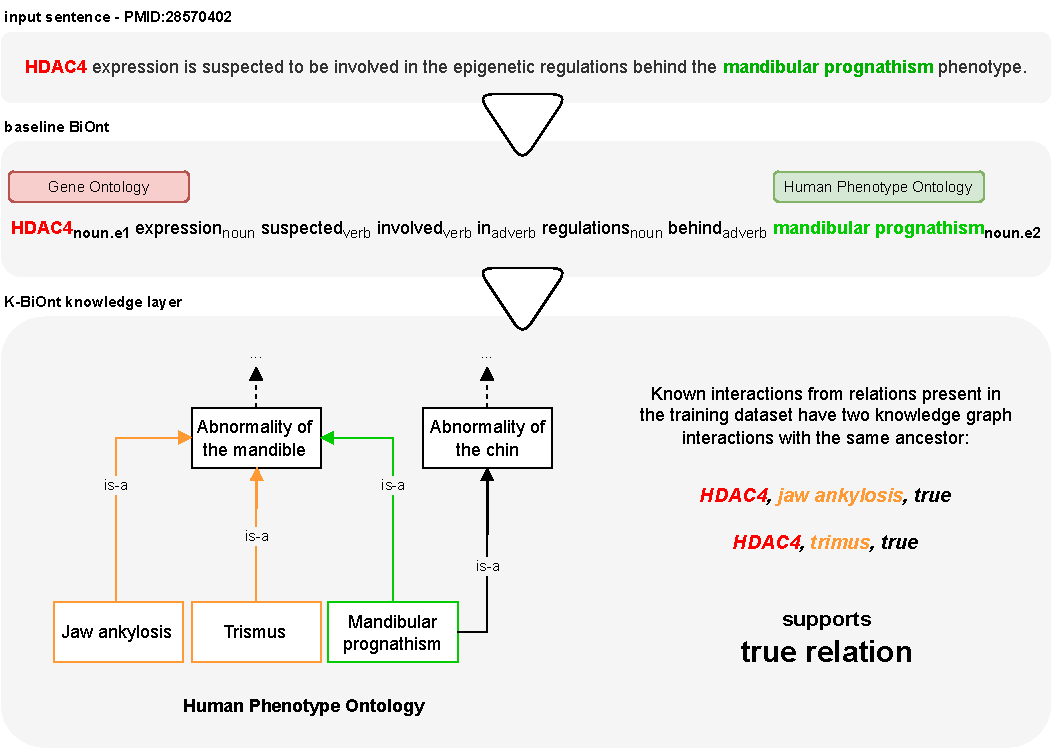
\includegraphics[width=\linewidth]{images/chapter_4/pipeline.pdf}}
\caption[General K-BiOnt Approach Pipeline]{General approach pipeline regarding the joint approaches BiOnt and the knowledge layer based on recommendation. We simplified the input sentence to facilitate reading comprehension (PMID:28570402).}
\label{fig:full_pipeline}
\end{figure*}

First, we proceed with the standard training process of the BiOnt model, which can be divided into three main stages after sentence tokenization: WordNet classes \citep{ciaramita2006broad}, word embeddings, and ontology embeddings. The ontology embedding stage represents the relations between the ancestors for each ontology concept corresponding to an entity. For instance, for the PGR-crowd dataset, the system links the entities to the HPO and GO biomedical ontologies, the DDI Corpus to the ChEBI ontology, and the BC5CDR Corpus to the ChEBI and DO ontologies with different coverage degrees, as discussed previously. The system uses a max pool layer fed into a dense layer through a sigmoid activation function, and a softmax layer outputs the probability for each class. The BiOnt model adds external entity knowledge through two channels of common ancestry and concatenation of ancestors. These knowledge channels aim to answer the questions: i) Do the entities in question share ancestors? (only applicable to relations between the same type of entities); and ii) Do the entities in question have ancestors that have established relations? The BiOnt model uses the answer to these two questions to support or discard a relation. However, our K-BiOnt knowledge layer goes deeper into the inferences that can support or discard a relation by answering: Do we have entities outside of the ones considered in the relation that we know that establish relations with one of the entities' ancestors? If yes, how many? In what capacity (true/negative)? And to what degree (e.g., 2, 3, or -5)? 


Thus, going back to the example in Figure~\ref{fig:full_pipeline}, our goal is to support or discard a relation between a gene \textit{HDAC4} and a human phenotype, \textit{Mandibular prognathism}. Yet, since their ancestors do not have known relations (excluding the BiOnt concatenation of ancestors' channel) and the entities are from different types (excluding the usage of the common ancestors' channel), the BiOnt knowledge layer does not provide information to support or discard this relation. However, since we know from the training set that the gene, \textit{HDAC4}, shares a true relation with both the \textit{Jaw ankylosis} and the \textit{Trimus} phenotype, and both of these entities have the same ancestor as the \textit{Mandibular prognathism} phenotype, we can support a true relation between \textit{HDAC4} and \textit{Mandibular prognathism}. Our knowledge layer considers translational relationships between \textit{users} and \textit{items}. This, in our example, means that for each human phenotype (\textit{item}) related to a gene (\textit{user}), we consider the whole subsequent ancestry of the phenotype until root to provide information on our gene.  


\subsection{Joint Evaluation}

To evaluate our approach, we created a confusion matrix table to compare the BiOnt model's output and the adjusted TUP model results against our gold standard test sets. This table served as a way for us to detect the main contributions of adding KG-based recommendation to a deep RE model (K-BiOnt) to all datasets.

One caveat is that an extracted relation between two entities is specific to the text where they are mentioned; however, in KG-based recommendation, the relation tag is specific to the entities it refers to. To overcome this issue, we primarily considered the label generated through the application of the baseline system to the normal text-bound RE dataset. We only changed the output if the modules (Deep Learning and Recommendation) disagreed with the label. Upon disagreement, we only altered the label if the Recommendation module assigned true and the baseline system false. Thus, only considering the Recommendation module input to capture an undetected connection.   
Table~\ref{tab:cross_validation} presents an example of a confusion matrix table for five distinct scenarios using relations from the PGR-crowd dataset. All true relations captured by KG-based recommendation were attributed with the final judgment of true independently of the Top@N. We only considered false relations in the final judgment if all model components agreed on the label false. Therefore, the BiOnt module component was preferred for the attributed label since it is based on the linguistic context of the relationship. The Recommendation module, based exclusively on knowledge regarding the target entities, was only considered for potential true labels that we hypothesize could not be retrieved solely on the linguistic context or were less frequent in the training data. 

\begin{table}[h]
\centering
  \caption[Confusion Matrix Example for Different K-BiOnt Scenarios]{An example of a confusion matrix table for five distinct scenarios using relations from the PGR-crowd dataset. FJ stands for Final Judgement and GS for Gold Standard}
  \begin{tabular}{lcccccc}
    \hline
    Relation (user-item) & BiOnt & Top@3 & Top@5 & Top@10 & FJ & GS\\
    \hline
    WNT7B-cancer & True & True & True & True & True & True \\
    \hline
    Adcy1-seizures & False & False & False & True & True & True \\
    \hline
    TRAPPC2-developmental delay & True & False & False & False & True & True \\
    \hline
    \rowcolor[gray]{0.9}
    IARS2-neuropathy & False & False & False & False & False & True \\
    \hline
    \rowcolor[gray]{0.9}
    SLC12A6-autosomal recessive & False & True & True & True & True & False \\
    \hline
  \end{tabular}
    \label{tab:cross_validation}
\end{table}

\section{Results and Discussion}

This section presents our assessment of the benefits of using KG-based recommendation as an added resource for RE systems in the biomedical domain. As a baseline, we compared the results of the baselines deep learning models BiOnt \citep{sousa2020biont} and BioBERT \citep{lee2020biobert} for RE with the adjusted TUP model \citep{10.1145/3308558.3313705} for item recommendation and the integration of BiOnt with TUP (K-BiOnt).


\subsection{Deep Learning Model}

Table~\ref{tab:biont_results} presents the results for the application of our three datasets to the deep learning models BiOnt and BioBERT. 

For BiOnt, the results were slightly different from the performances reported on the original work for the DDI Corpus \citep{herrero2013ddi}, but almost identical for the PGR-crowd dataset \citep{sousa2020hybrid}. We can justify the DDI Corpus performance differences ($\approx$ 4\% in F1) with our use of the updated ChEBI version that has fewer alignments with the entities in the original dataset. The PGR-crowd has a significant imbalance of true/false relations, with the majority of relations being true and the DDI and BC5CDR Corpora share the same imbalance but in favour of the false relations (Table~\ref{tab:dl_statistics}), which can affect the performance of these datasets differently, despite the BiOnt model ability to assign class weights.

As for the BioBERT system's PGR-crowd dataset and the BC5CDR Corpus results were very similar to the BiOnt's model performance. However, given the class imbalances of all three datasets, it should be possible to alter class weights. Still, BioBERT's loss function does not allow this flexibility, possibly undermining their results. The BioBERT system significantly outperformed the BiOnt model for the DDI Corpus, despite the class imbalances. 

\begin{table}[h]
\centering
  \caption[Results for Relation Extraction using BiOnt and BioBERT Systems]{Overall results regarding the BiOnt and BioBERT systems. P stands for Precision, and R for Recall}
  \label{tab:biont_results}
  \begin{tabular}{llccc}
    \hline
    Dataset & System & P (\%) & R (\%) & F1 (\%) \\
    \hline
    \multirow{2}{*}{PGR-crowd} & BioBERT & 80.04 & 99.22 & 88.60 \\
    & BiOnt & 81.30 & 97.55 & 88.69  \\
    \hline
    \multirow{2}{*}{DDI Corpus} & BioBERT & 86.61 & 87.23 & 86.92 \\
    & BiOnt & 61.85 & 73.24 & 67.06 \\
    \hline
    \multirow{2}{*}{BC5CDR Corpus} & BioBERT & 59.78 & 72.67 & 65.60 \\
    & BiOnt & 63.96 & 71.73 & 67.62 \\
    \hline
  \end{tabular}
\end{table}


\subsection{Knowledge Graph-based Recommendation}

Table~\ref{tab:ir_results} presents the results for the adapted TUP model using the soft item recommendation strategy mentioned in Section 3.2.3. TUP authors \citep{10.1145/3308558.3313705} state that the peak performance for their model is when the average number of ratings for users ranges from 100 to 200. This range is far from our average number of ratings for both datasets (2 for PGR-crowd, 10 for DDI Corpus, and 4 for the BC5CDR Corpus). Thus, we believe that more training data allied with less sparsity would enhance our results further. Also, the higher overall results for the PGR-crowd demonstrate the importance of item-entity alignments since all items (i.e., human phenotypes) were linked to the HPO \citep{kohler2019expansion}. In contrast, on the DDI and BC5CDR Corpora, only 47.8\% and 26.0\% of the items could be linked to the ChEBI \citep{herrero2013ddi} and DO \citep{schriml2012disease} ontologies, respectively, leading to a drop in performance.  

\begin{table}[h]
\centering
  \caption[Results for Item Recommendation with TUP]{Overall results regarding the TUP model for Item Recommendation. P stands for Precision, and R for Recall}
  \label{tab:ir_results}
  \begin{tabular}{lccccc}
    \hline
    Dataset & P@10 (\%) & R@10 (\%) & F1@10 (\%) & Hit ratio@10 (\%) & nDCG@10 (\%) \\
    \hline
    PGR-crowd & 3.72 & 32.10 & 6.59 & 35.96 & 19.33 \\
    \hline
    DDI Corpus & 1.90 & 2.40 & 1.90 & 18.70 & 8.20 \\
    \hline
    BC5CDR Corpus & 0.53 & 2.24 & 0.79 & 5.28 & 2.37 \\
    \hline
  \end{tabular}
\end{table}


\subsection{Joint Evaluation}

Table~\ref{tab:final_results} presents the final results by adding the adjusted TUP model recommendation to the BiOnt model (K-BiOnt), considering  top@3, top@5, and top@10 recommendations. These results are a reflection of the results of the confusion matrix tables created as described in the example of Table~\ref{tab:cross_validation}.  

\begin{table}[h]
\centering
  \caption[K-BiOnt Final Results]{Final results by adding the adjusted TUP model recommendations to the BiOnt model (K-BiOnt), considering top@3, top@5, and top@10 recommendations. P stands for Precision, and R for Recall}
  \label{tab:final_results}
  \begin{tabular}{llccc}
    \hline
    Dataset & Configuration & P (\%) & R (\%) & F1 (\%) \\
    
    \hline
    \multirow{4}{*}{PGR-crowd} & BiOnt & \textbf{81.30} & 97.55 & 88.69 \\
    & + Top@3 & 81.23 & 97.90 & \textbf{88.79} \\
    & + Top@5 & 80.98 & \textbf{98.17} & 88.75 \\
    & + Top@10 & 80.98 & \textbf{98.17} & 88.75 \\
    
    \hline
    \multirow{4}{*}{DDI Corpus} & BiOnt & \textbf{61.85} & \textbf{73.24} & \textbf{67.06} \\
    & + Top@3 & 61.85 & 73.24 & 67.06 \\
    & + Top@5 & 61.85 & 73.24 & 67.06 \\
    & + Top@10 & 61.85 & 73.24 & 67.06 \\
    
    \hline
    \multirow{4}{*}{BC5CDR Corpus} & BiOnt & 63.96 & 71.73 & 67.62 \\
    & + Top@3 & 63.96 & 71.73 & 67.62  \\
    & + Top@5 & 64.15 & 72.34 & 68.00  \\
    & + Top@10 & \textbf{64.45} & \textbf{73.25} & \textbf{68.56} \\


    \hline
  \end{tabular}
\end{table}


For the PGR-crowd dataset, the average number of ratings per \textit{user} entity is 2. A false relation usually appears only once being rated with $-1$ and not a lower number, which is insufficient to indicate to the model that the \textit{user} entity is unrelated to an \textit{item} entity. An approach that we could study in the future is creating negative sampling using false relations, not the traditional random sampling for negative observations associated with implicit feedback. The added performance of TUP over the BiOnt model (K-BiOnt) holds for all Top@N. However, the number of false positive relations increases with the subsequent decrease in performance for Top@5 and Top@10. Although, after closer inspection to the added false positives, for the majority of them, the \textit{item} entity human phenotype is under the \textit{Mode of inheritance} category of HPO, not under \textit{Phenotypic abnormality}. This last branch is the most developed branch within the HPO and is of more interest to researchers. Likewise, the BC5CDR Corpus also increased performance compared to the BiOnt baseline for Top@5 and Top@10 despite the low TUP performance, which indicates potential for a more impactful approach following improvement in linking the entities to KG identifiers. 

For the DDI Corpus, the results are identical across all Top@N (the BioBERT baseline) since we could not capture a true positive through item recommendation within the first ten recommendations. 


\subsection{Ablation Study}

To study the impact of knowledge graph coverage, we chose the dataset with the lowest value in coverage (BC5CDR Corpus). We created the recommendation module only taking into account the 156 items linked to DO ontological concepts. Table~\ref{tab:final_results_ab} presents the results for this study. 

\begin{table}[h]
\centering
  \caption[Ablation Study Results Regarding the TUP model for Item Recommendation]{Ablation study results regarding the TUP model for Item Recommendation for the Full Dataset and the KG covered Subset of the BC5CDR Corpus. P stands for Precision and R for Recall}
  \label{tab:final_results_ab}
  \begin{tabular}{lccccc}
    \hline
    Dataset & P@10 (\%) & R@10 (\%) & F1@10 (\%) & Hit ratio@10 (\%) & nDCG@10 (\%) \\
    \hline
    Full BC5CDR & 0.53 & 2.24 & 0.79 & 5.28 & 2.37 \\
    \hline
    Subset BC5CDR & 0.79 & 4.87 & 1.32 & 7.92 & 5.62 \\
    \hline
  \end{tabular}
\end{table}

By Table~\ref{tab:final_results_ab}, we can verify that the presence of only ontological covered items, even if in a small number, is enough to impact the performance of item recommendation, almost doubling our previous results. Even if there was no significant impact on the K-Biont model due to the small number of items, we know that augmenting the covered items through a more robust concept normalization step can improve the K-BiOnt performance. 

\subsection{Impact on RE}

We decided to perform an error analysis on the performance of the PGR-crowd dataset, comparing the baselines BioBERT and BiOnt to our approach K-BiOnt to measure their actual impact on the RE task. We found that more true relations were identified by considering relations that the KG-based recommendation model recommended.  

In the PGR-crowd dataset, the \textit{item} entities (i.e., human phenotypes) are all linked to the HPO, with subsequent complete coverage of the KG entities over the \textit{item} entities. The full coverage translated to a higher contribution of the recommendation module to the RE task. Figure~\ref{fig:example_r} illustrates one of those true relations detected by the recommendation module and missed by the BiOnt model. Note that our models only added true relations recommended with the adjusted TUP at Top@3. All other experiments also recommended false positives, undermining the recommendation module benefits.

\begin{figure*}[!h]
\centerline{
\includegraphics[width=\linewidth]{images/chapter_4/example.pdf}}
\caption[An Example of a True Relation Detected by the Recommendation Module]{An example of a true relation detected by the recommendation module from the PGR-crowd dataset from article PMID:27103084. The phenotype entity is linked to the HPO ontology (HP:0001263), and the gene entity is linked to the NCBI gene database (55714). We simplified the sentence to facilitate reading comprehension.}
\label{fig:example_r}
\end{figure*}

These results show the advantage of adding recommendations to RE, mainly to populate knowledge bases of gold standard relations, where the goal is not only to identify the relation that is explicitly mentioned in the text but to find every true relation that we can derive from it. The success of the recommendation module is explained by the exploration of KGs that allows the RE process to consider the connections between the associated KG.  

However, existing KGs are far from complete, limiting the knowledge we can transfer into RE systems. Considering this limitation, \cite{10.1145/3308558.3313705} aligned item recommendation (TUP) with KG completion (TransH). KG completion is a field in accelerated popularity given its relevance for question answering tasks \citep{10.1145/3132847.3132977,10.1145/3289600.3290956}, but also to search entities and their relations in text \citep{ji2020survey}. This field should be considered for future exploration of added knowledge to biomedical RE to further enhance the recommendation of less frequent relations.  


\section{Conclusion and Future Work}

This paper proposed a new recommendation-based complementary approach to deep learning biomedical RE that considers biomedical ontologies as additional sources of information. The KG-based recommendation pipeline presented in this work takes advantage of \textit{user} entity-\textit{item} entity interactions as well as knowledge graphs that can be linked to \textit{item} entities. In our case study, the biomedical KGs were HPO, ChEBI, and DO. We performed experiments using both item recommendation algorithm on its own and as an added module to a deep biomedical RE system. We present the benefits of using both methods simultaneously and the RE task's added value. Our results show that KG-based recommendations can be a valuable asset to biomedical RE by detecting previously undiscovered true relations between biomedical entities. However, the low coverage of the associated KGs damages performance.

Additionally, we produced three recommendation datasets in the format $<$user-item-rating$>$ for human phenotype and gene relations, drugs/chemicals interactions, and drugs/chemicals and diseases relations, attributing a rating for each user-item pair. We also presented a comprehensive pipeline for creating a biomedical RE system using KG-based recommendation (K-BiOnt). Ultimately, we demonstrated that adding recommendations can increase deep biomedical RE models' performance by considering external sources of knowledge when they have sufficient coverage of the domain.

Biomedical RE datasets usually do not describe more than one type of relation. However, upon the availability of a dataset describing more types of labelled relations, a multi-graph approach could be employed linking each \textit{item} entity to their respective ontological identifier. Even though we could argue that our representation of the ratings between user-item pairs is not representative of the real world, it is a cross-approach problem. Current deep learning approaches to biomedical RE also take labelled data to create models where the distribution is not a representation of real-world data and where a lot of less frequent associations are missed. 
In the future, the approach could be expanded by considering other types of relations between biomedical entities and by applying it to different types of baseline systems (i.e., BioBERT). Another angle to be explored could be adding more biomedical ontologies, including possible interconnections between multiple ontologies, that could expand our KGs even further by increasing the number of preferences. Also, upon availability within biomedical ontologies, another complementary route could be adding informative axioms such as \textit{disjointness} and studying the effect of ontological depth.

\hypertarget{5}{}

\rhead{K-RET: Knowledgeable Biomedical Relation Extraction System}
\lhead{Chapter 5}

\chapter[K-RET: Knowledgeable Biomedical Relation Extraction System]
{\huge K-RET: Knowledgeable Biomedical Relation Extraction System \\
\Large \textmd{Diana F. Sousa and Francisco M. Couto}}

\vspace{-1.6cm}

% Gray Line
\begingroup
\color{black}
\par\noindent\rule{\textwidth}{0.4pt}
\endgroup

\noindent{This chapter tackles Objective 1 by integrating knowledge to expand text training data of BERT-based models. This work is particularly relevant to tackle the main hypothesis of this thesis since it is the most recent and includes all expertise acquired throughout the doctoral work. Corresponds to the journal article:} 

\begin{itemize}[label=]
    \item{\textbf{Sousa, D. F.} and Couto, F. M. (2023). \textbf{K-RET: Knowledgeable Biomedical Relation Extraction System}. Bioinformatics, 39(4):1-8. (Q1 Scimago) \citep{sousa2023k}}
\end{itemize}

\textbf{Abstract.} \textbf{Motivation:} Relation Extraction (RE) is a crucial process to deal with the amount of text published daily, for example, to find missing associations in a database. RE is a text mining task for which the state-of-the-art approaches use bidirectional encoders, namely, BERT. However, state-of-the-art performance may be limited by the lack of efficient external knowledge injection approaches, with a larger impact in the biomedical area given the widespread usage and high quality of biomedical ontologies. This knowledge can propel these systems forward by aiding them in predicting more explainable biomedical associations. With this in mind, we developed K-RET, a novel, knowledgeable biomedical relation extraction system that, for the first time, injects knowledge by handling different types of associations, multiple sources and where to apply it, and multi-token entities.\\
\textbf{Results:} We tested K-RET on three independent and open-access corpora (DDI, BC5CDR, and PGR) using four biomedical ontologies handling different entities. K-RET improved state-of-the-art results by 2.68\% on average, with the DDI Corpus yielding the most significant boost in performance, from 79.30\% to 87.19\% in F-measure, representing a p-value of $2.91 \times 10^{-12}$.\\
\textbf{Availability:} \url{https://github.com/lasigeBioTM/K-RET}

\section{Introduction}

With the exponential increase in the number of research articles published in the last decades, researchers find it hard to keep up with all relevant information for their respective fields. The overwhelming number of research papers, particularly in the biomedical field, frequently makes it impossible for researchers and clinicians to be aware of all established entity associations and dissociations. This unawareness often leads to experimental repetition to prove or disprove hypotheses already studied. Further, even if the hypothesis is unique or new, the same inference could often be retrieved from knowledge about experiments done on similar entities. Automated biomedical Relation Extraction (RE) is a fundamental step toward aiding these researchers and clinicians in saving time and focusing their work on genuinely novel associations.

Through the years, several approaches have been employed to tackle biomedical RE, from straightforward rule-based approaches \citep{rinaldi2007mining,kilicoglu2020broad} to entire machine learning dedicated systems \citep{houssein2021machine,abdelkader2021machine}, in which deep learning played a significant role \citep{dash2020deep}. Successively, these approaches became more specialized in targeting multiple types of biomedical associations from protein-protein relations \citep{kim2006biocontrasts} to human phenotype-gene causality \citep{song2019leveraging,sousa2022biomedical}. BERT \citep{devlin2019bert} and their domain derivatives, such as BioBERT \citep{lee2020biobert}, SciBERT \citep{scibert}, and PubMedBERT \citep{gu2021domain} are the current state-of-the-art employed solutions. They not only successfully extract multiple types of relations from the text but can also, using their pre-trained models, be easily integrated into newer systems targeting different Natural Language Processing (NLP) tasks, such as Named-Entity Recognition (NER) \citep{nasar2021named}, Named-Entity Linking (NEL) or Normalization \citep{ruas2022nilinker}, and Question Answering (QA) \citep{do2022developing}.

However, there are some caveats for most biomedical RE systems. The first limitation is their focus and specialization on one specific type of association \citep{hu2021survey}, with some notable exceptions that are flexible to target more than one type \citep{song2019leveraging,sousa2020biont,sousa2022biomedical}. The second limitation is that systems' results frequently lack an explanation. One can not easily understand how a relation was found and what inferences a particular model made to reach an output. Finally, in close connection with making systems explainable, the third more relevant limitation is their general disregard for the vast repertoire of biomedical dedicated knowledge bases, particularly in the form of ontologies. This multitude of organized biomedical knowledge is freely available, but most systems still rely only on the information from the training data. Some exemptions recently made some strides into using knowledge in the general domain \citep{liu2020k} and the biomedical/clinical domain \citep{hao2020enhancing}. However, these are still limited in the domain's specificity and inflexible to adding different or more structured knowledge.  

Some of the most notary examples of organized biomedical knowledge are the Gene Ontology (GO) \citep{ashburner2000gene,gene2019gene}, the Human Phenotype Ontology (HPO) \citep{kohler2021human}, the Human Disease Ontology (DO) \citep{schriml2022human}, the Chemical Entities of Biological Interest (ChEBI) \citep{degtyarenko2007chebi}, and the Unified Medical Language System (UMLS) \citep{bodenreider2004unified}. Respectively, these organized resources described connections between gene function descriptors, human phenotypes, human diseases, chemicals of biological interest, and clinical entities. 

The work of \cite{liu2020k} is a recent and successful attempt
 for knowledge incorporation into multiple open and specific-domain tasks. Their K-BERT system was able to incorporate domain knowledge without creating a heterogeneous embedding space. The novelty in their approach is the creation of a knowledge layer that injects knowledge directly into the sentence. Then, they perform sentence tree re-arrangement before the embedding layer, with the addition of a soft-position embedding and a visible matrix to target possible readability problems from the re-arrangement. Also, it does not require pre-training of the BERT models it supports, making it suitable for users with limited computational resources \citep{zhao2019uer}. However, their system has some major constrictions. First, the authors do not apply their approach to the RE task for the open or biomedical-specific domains. Second, the knowledge injection can only be used for single tokens within the sentence tree, making it miss knowledge associated with multi-token entities that are most prevalent in the biomedical domain. Third, the application of their system only allows for the injection of knowledge from one knowledge source, constraining data that intersects one or more domains (e.g., patient case reports that mention both the procedures done and the phenotypes associated with the patients). Finally, there is no possibility of injecting target knowledge into the entities of interest; one must always apply knowledge to all possible sentence tokens.   

In this work, we designed a new approach to knowledge injection that is able to address the challenges stated in the last paragraph to create K-RET, a knowledgeable biomedical RE BERT-based system. K-RET is a flexible biomedical RE system, allowing for the use of any pre-trained BERT-based system (e.g., SciBERT and BioBERT) to inject knowledge in the form of knowledge bases from a single source or multiple sources simultaneously. This knowledge can be applied to various contextualizing tokens or just to the tokens of the candidate relation for single and multi-token entities. 

K-RET effectively improves the performance of baseline biomedical BERT-based models by an average of 2.68\% on all datasets (DDI \citep{herrero2013ddi,segura2014lessons}, BC5CDR \citep{li2016biocreative}, and PGR-crowd \citep{sousa2019silver,sousa2020hybrid} Corpora). The most successful configuration is applying contextualised knowledge by adding two knowledge base entities per possible domain entity within each sentence tree (i.e., DDI Corpus plus ChEBI). This work resulted in the following main contributions:\vspace*{1pt}

\begin{itemize}
\item K-RET, a knowledgeable biomedical RE system that allows for the integration of any pre-trained BERT-based system.
\item Approach to flexible injection of knowledge with multi-options:
\begin{enumerate}
    \item association of knowledge to single or multi-token entities in the sentence tree;
    \item add more than one knowledge source to inject knowledge of different domains;
    \item injection of knowledge into targeted or multiple contextualizing tokens in a sentence tree. \vspace*{1pt} 
\end{enumerate}
\end{itemize}

In the following section, System and Methods, we describe K-RET, formally presenting the main architectural features. In Section 3, Implementation, we describe the resources used (datasets and knowledge bases), parameters, training details and the main results of different system configurations. These configurations are the baseline (i.e., without knowledge) and the use of target versus contextualized knowledge within three different biomedical RE datasets. Sections 4 and 5 discuss the previous results with targeted ablation studies and present the main conclusions and future work. 


\section{System and Methods}

In this section, we will present our system K-RET, represented in Figure \ref{fig:51}. We will describe each new system component and how they differ from the implementations from both BERT \citep{devlin2019bert} and K-BERT \citep{liu2020k}, which was built using the UER platform \citep{zhao2019uer}, starting by defining the general Notation and then detailing our additions in Architecture.   

\begin{figure}[hbt!]
\centerline{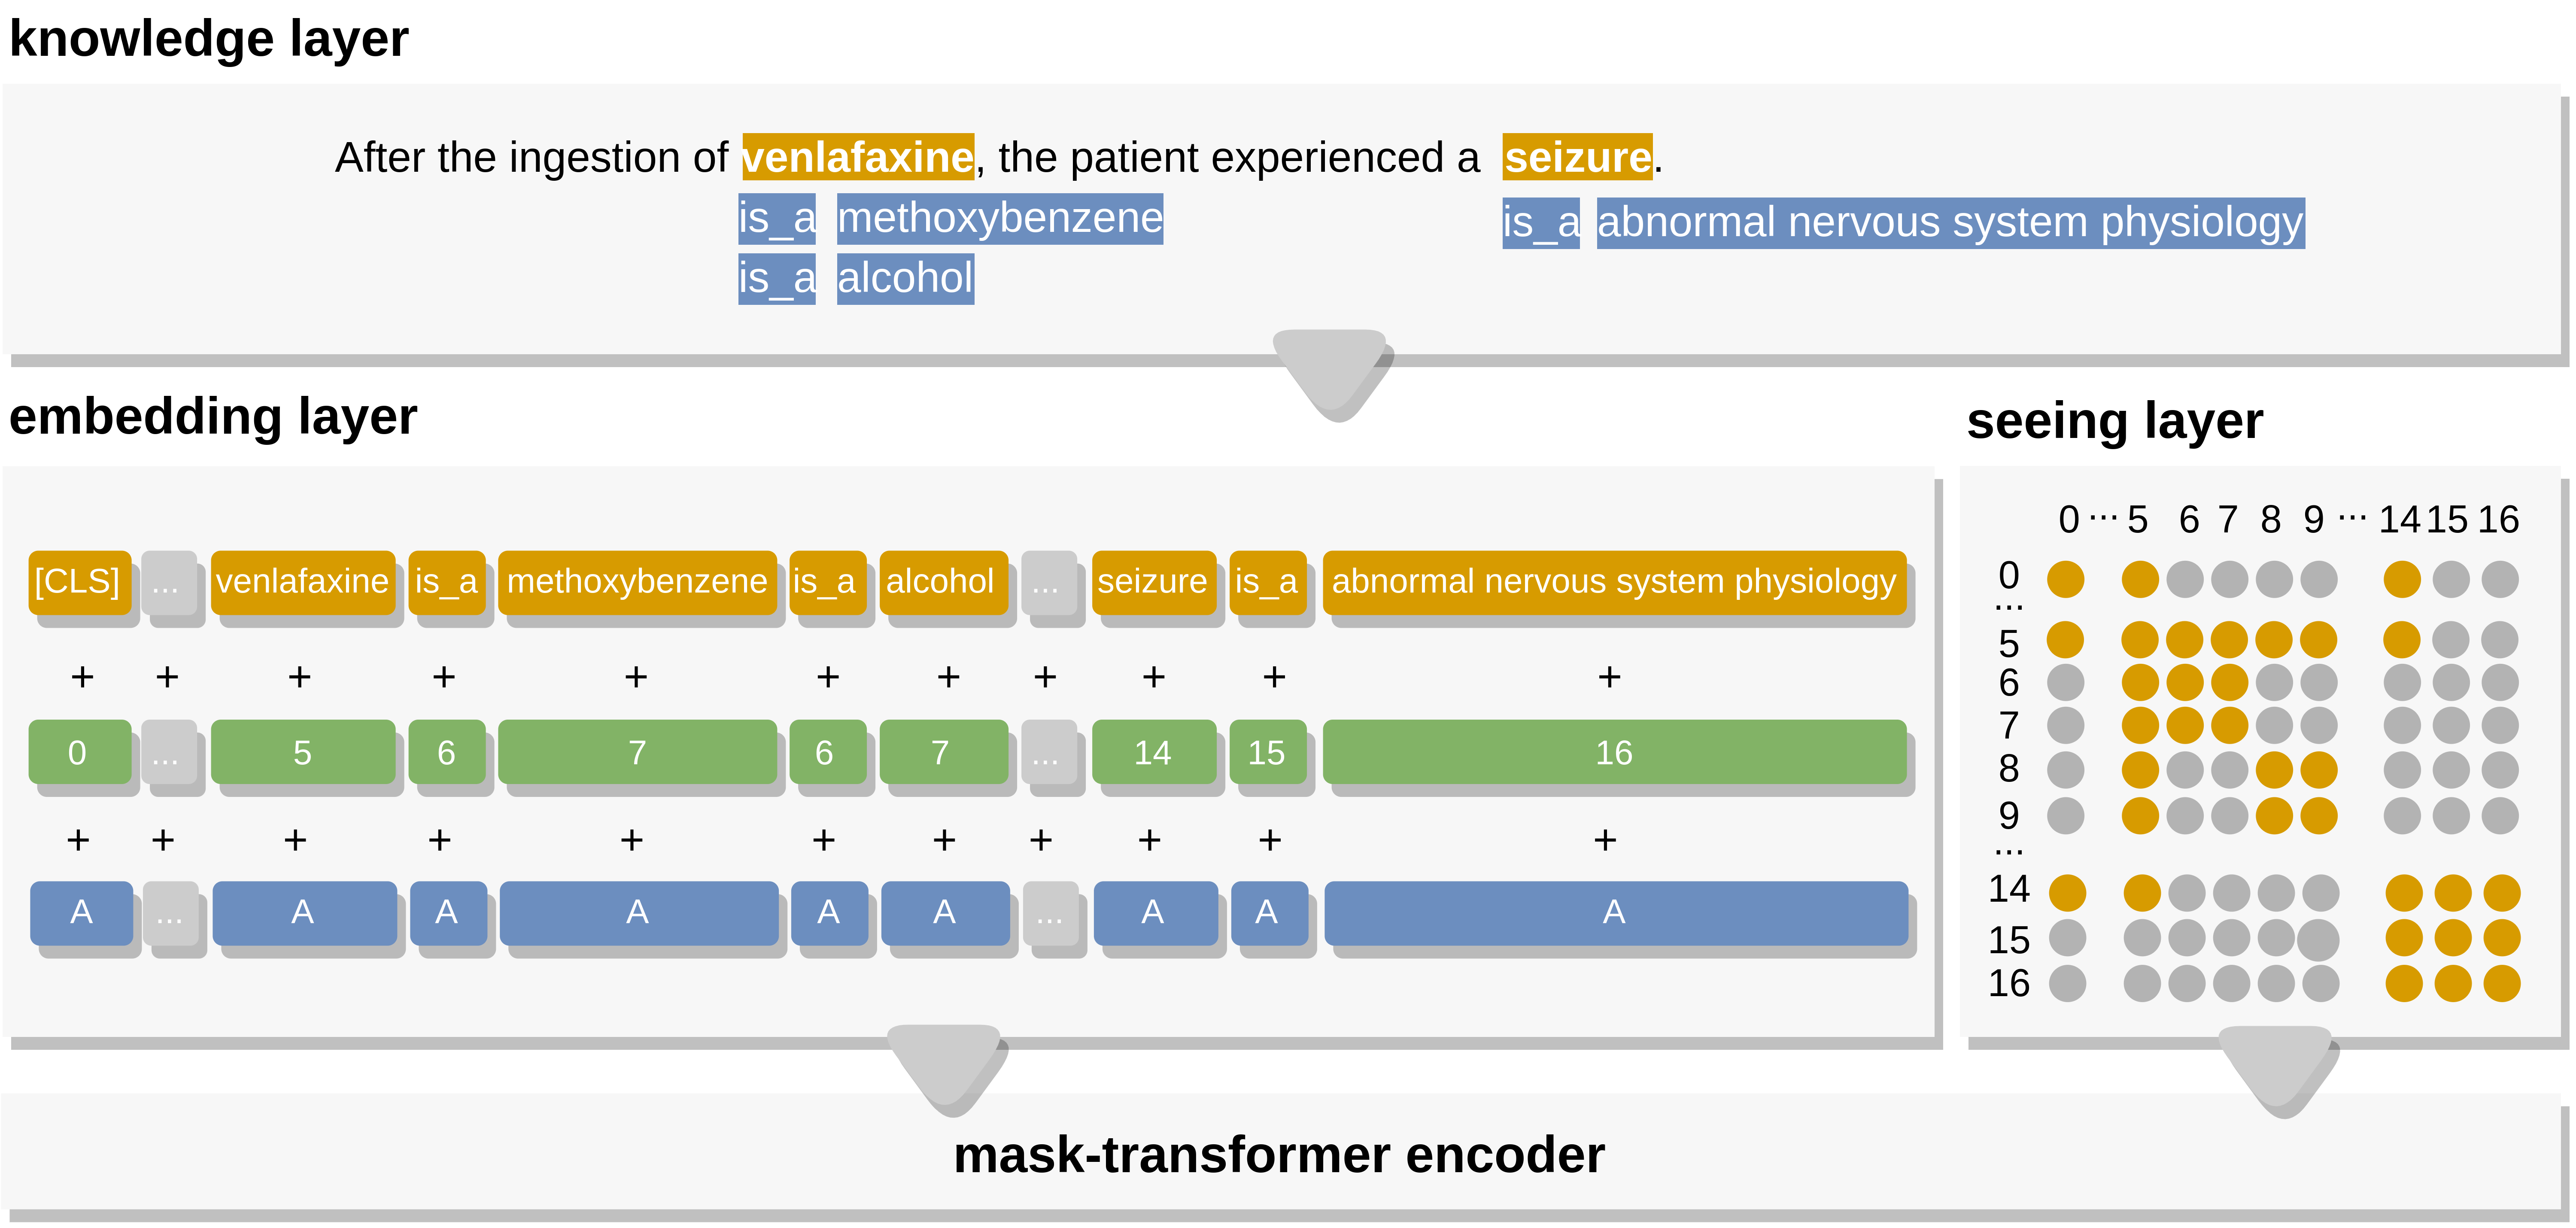
\includegraphics[width=\linewidth]{images/chapter_5/kret_methodology.png}}
\caption[Structured Layer Representation of K-RET]{The structured layer representation of K-RET. In the pipeline, we retrieved a sentence from a biomedical relation extraction dataset with delimited target entities: venlafaxine and seizure. We added a Knowledge layer to these entities from associations made with their respective domain ontologies, the Chemical Entities of Biological Interest (ChEBI) and the Human Disease Ontology (DO). In the Embedding layer, the tokens are flattened into a sequence for token embedding. Then, the soft-position embedding is used along with the token embedding, and the tokens are tagged with A for segment embedding. The orange circles correspond to visible tokens in the Seeing layer, while the grey circles correspond to invisible ones. For instance, in row five, venlafaxine(5) is visible to all tokens except the last two: is\_a(15) and abnormal nervous system physiology(16). Finally, both layers, Embedding and Seeing, are fed to the Mask-transformer, corresponding to a stack of multiple mask-self-attention blocks. This last layer is masked to prevent the transformer from receiving structural information of the sentence tree. The sentence was simplified for readability purposes.}\label{fig:51}
\end{figure}

\subsection{Notation}

We define a sentence $s$ as a sequence of tokens $t_{i}$, with length $n$:

\begin{equation}
s = \{t_{0}, t_{1}, t_{2}, ..., t_{n}\}\label{eq:01}
\end{equation}

Each token can represent one or more words that are included in the vocabulary $V$, $t_{i} \in V$.  
The Knowledge Base, $K$, consists of a collection of triples, $e$:

\begin{equation}
e = (t_{i}, r_{j}, t_{k})\label{eq:02}
\end{equation}

where $t_{i}$ and $t_{k}$ are the descriptors of the entities, $r_{j}$ the relation between them, $r_{j} \in V$, and $e \in K$.


\subsection{Architecture}

The model architecture of K-RET is divided into four modules. The first module, a Knowledge layer, injects knowledge from the knowledge base in triples, expanding the original sentence into a knowledgeable sentence tree. The sentence tree is fed into simultaneously the Embedding layer (second module) and the Seeing layer (third module). Then, it is converted to token-level embedding representation and a visible matrix, as presented in Figure \ref{fig:51}. This matrix acts as a control to prevent the injected knowledge from altering the meaning of the original sentence with excessive knowledge. The embedding representation can then be fed into the Mask-transformer (fourth module). 

K-BERT created a knowledge layer that injects knowledge and performs sentence tree conversion. On the other hand, our new knowledge layer was designed to address the three previously mentioned challenges. We detail how we tackled those limitations in the next sections: Multi-token entities, Multiple knowledge bases, and Contextual and targeted knowledge. Beyond the knowledge layer, we made changes to the original predictive pipeline by allowing the addition of class weights, a new type of data format, and the inclusion of any BERT-based pre-trained model using the UER framework.


\subsubsection{Multi-token Entities}

For multi-token entities, we first considered all combinations of single tokens to generate all possible multi-tokens in the same input sentence. Thus, if a sentence has a number of tokens of $10$, the number of combinations possible would be $55$. This number can vary if the sentence has punctuation or other special characters. Then, through a lookup table, we can add knowledge to all combinations we can match in the chosen knowledge base, keeping the longest combinations of tokens (with increased specificity) when there is overlap. Finally, we reconstruct the sentence tree through a sliding window that goes through all the combinations with and without knowledge. 

We introduced a multi-token entities option to address the limitation of only using one token, both in the sentence itself and in the knowledge to be injected. As it stands, the model did not allow associating knowledge to more than one token (e.g., \textbf{aralkylamino compound} (original sentence tokens) \textit{is\_a} organic amino compound (added knowledgeable token)) nor associate multiple word knowledge to one or more words in the original sentence (e.g., dopamine (original sentence token) \textit{is\_a} \textbf{aralkylamino compound} (added knowledgeable tokens)). 


\subsubsection{Multiple Knowledge Bases}

To accommodate multiple knowledge bases, we expanded the number of lookup tables mentioned in the previous section. Thus, if we use more than one knowledge base, K-RET will look at the sentence a number of times corresponding to the number of knowledge bases. If there is complete or partial overlap between two or more competing knowledgeable tokens associated with an entity in the sentence and the number of association tokens surpasses the number of maximum tokens defined at the start, we keep the ones with the highest information content. 

The multiple knowledge bases option resolves the limitation of using only one knowledge base at a time. Therefore if we have, as in the biomedical domain, knowledge bases targeting different types of entities, we can choose which ones we want to use to inject knowledge into the original sentence. 


\subsubsection{Contextual and Targeted Knowledge}

Finally, we decided to add the possibility of only injecting knowledge into the entities in consideration for relation assessment, maintaining the native option of adding knowledge to all entities present in the sentence. 

To define the targeted entities, we used the tags \texttt{<e>} and \texttt{</e>} to delimit the entities in the candidate relation. The tags allowed injecting knowledge directly into the candidate entities. K-RET ignores those tags when using contextual knowledge for knowledge injection, adding knowledge to entities as described previously. 

Hence, as a result of the three additions, given an input sentence $s = \{t_{0}, t_{1}, t_{2}, ..., t_{n}\}$ and one or more knowledge bases, our knowledge layer outputs a sentence tree:

\begin{equation}
st = \{t_{0}, t_{1}, t_{2}, ..., t_{i}\{(r_{i0}, t_{i0}), ..., (r_{ik}, t_{ik})\}, ..., t_{n}\}\label{eq:03}
\end{equation}

which results from (1) querying all entity names involved in the sentence $s$, independently from their length and selecting correspondent triples from $K$, and (2) adding the triples to their correspondent position. Figure \ref{fig:51} illustrates the structure of the sentence tree $st$ and an example retrieved from our data. While the sentence tree can have multiple branches, the depth is fixed to 1, not deriving branches iteratively to better preserve the original sentence meaning. 


\section{Implementation}

In this paper, we used three openly-available RE datasets to train K-RET: DDI Corpus \citep{herrero2013ddi,segura2014lessons} (drug-drug interactions), PGR-crowd Corpus \citep{sousa2019silver,sousa2020hybrid} (human phenotype-gene interactions), and BC5CDR Corpus \citep{li2016biocreative} (chemical-disease associations). Along with the written information in these RE datasets, we used four knowledge bases related to the four types of entities identified within those datasets to add extra entity information to the K-RET system. These knowledge bases are Human Phenotype Ontology (HPO) \citep{kohler2021human}, Disease Ontology (DO) \citep{schriml2022human}, Chemical Entities of Biological Interest (CHEBI) \citep{degtyarenko2007chebi}, and Gene Ontology (GO) \citep{ashburner2000gene,gene2019gene}. In this section, we present the different experiments made to access our system using the aforementioned datasets and knowledge bases, with parameters and training details tuned for the specificities of each dataset. We also explore and present the results for the usage of full knowledge or just entity knowledge, as described in the previous section. 


\subsection{Datasets}

Table~\ref{Tab:01} represents the relations types and counts for each dataset. The \textit{no\_relation} label accounts for entities present in the same sentence but that do not share a relation. The commonly used DDI Corpus presents four types of relations: \textit{effect} to describe an effect or pharmacodynamics mechanism, \textit{mechanism} to describe a pharmacokinetic mechanism, \textit{advice} to describe semantic relations between drugs regarding recommendation, and \textit{int} for relations where there is no further information. Both the PGR-crowd and BC5CDR Corpora are binary in terms of relation classification. These two datasets only classify if the relation is present (\textit{true}) or not (\textit{false}). Figure \ref{fig:52} presents an example sentence for each dataset. 

\begin{table}[h]
\centering
  \caption[Main Statistics of the Relation Extraction Corpora]{The main statistics of DDI Corpus, PGR-crowd Corpus, and BC5CDR Corpus
regarding the relation extraction task}
  \label{Tab:01}
\begin{tabular}{lccccc}
\hline 
\multirow{3}{*}{Dataset} & \multicolumn{4}{c}{Relation type} & \\\cline{2-6}
 & \multicolumn{4}{c}{True} & \multirow{2}{*}{No-relation / False}\\\cline{2-5}
 & Effect & Advice & Mechanism & Int &\\\hline
DDI & 2026 & 1616 & 1047 & 278 & 29245\\
PGR-crowd & 5498 & $-$ & $-$ & $-$ & 626\\
BC5CDR & 1448 & $-$ & $-$ & $-$ & 2294\\\hline
\end{tabular}
\end{table}

\begin{figure}[h]%figure2
\centerline{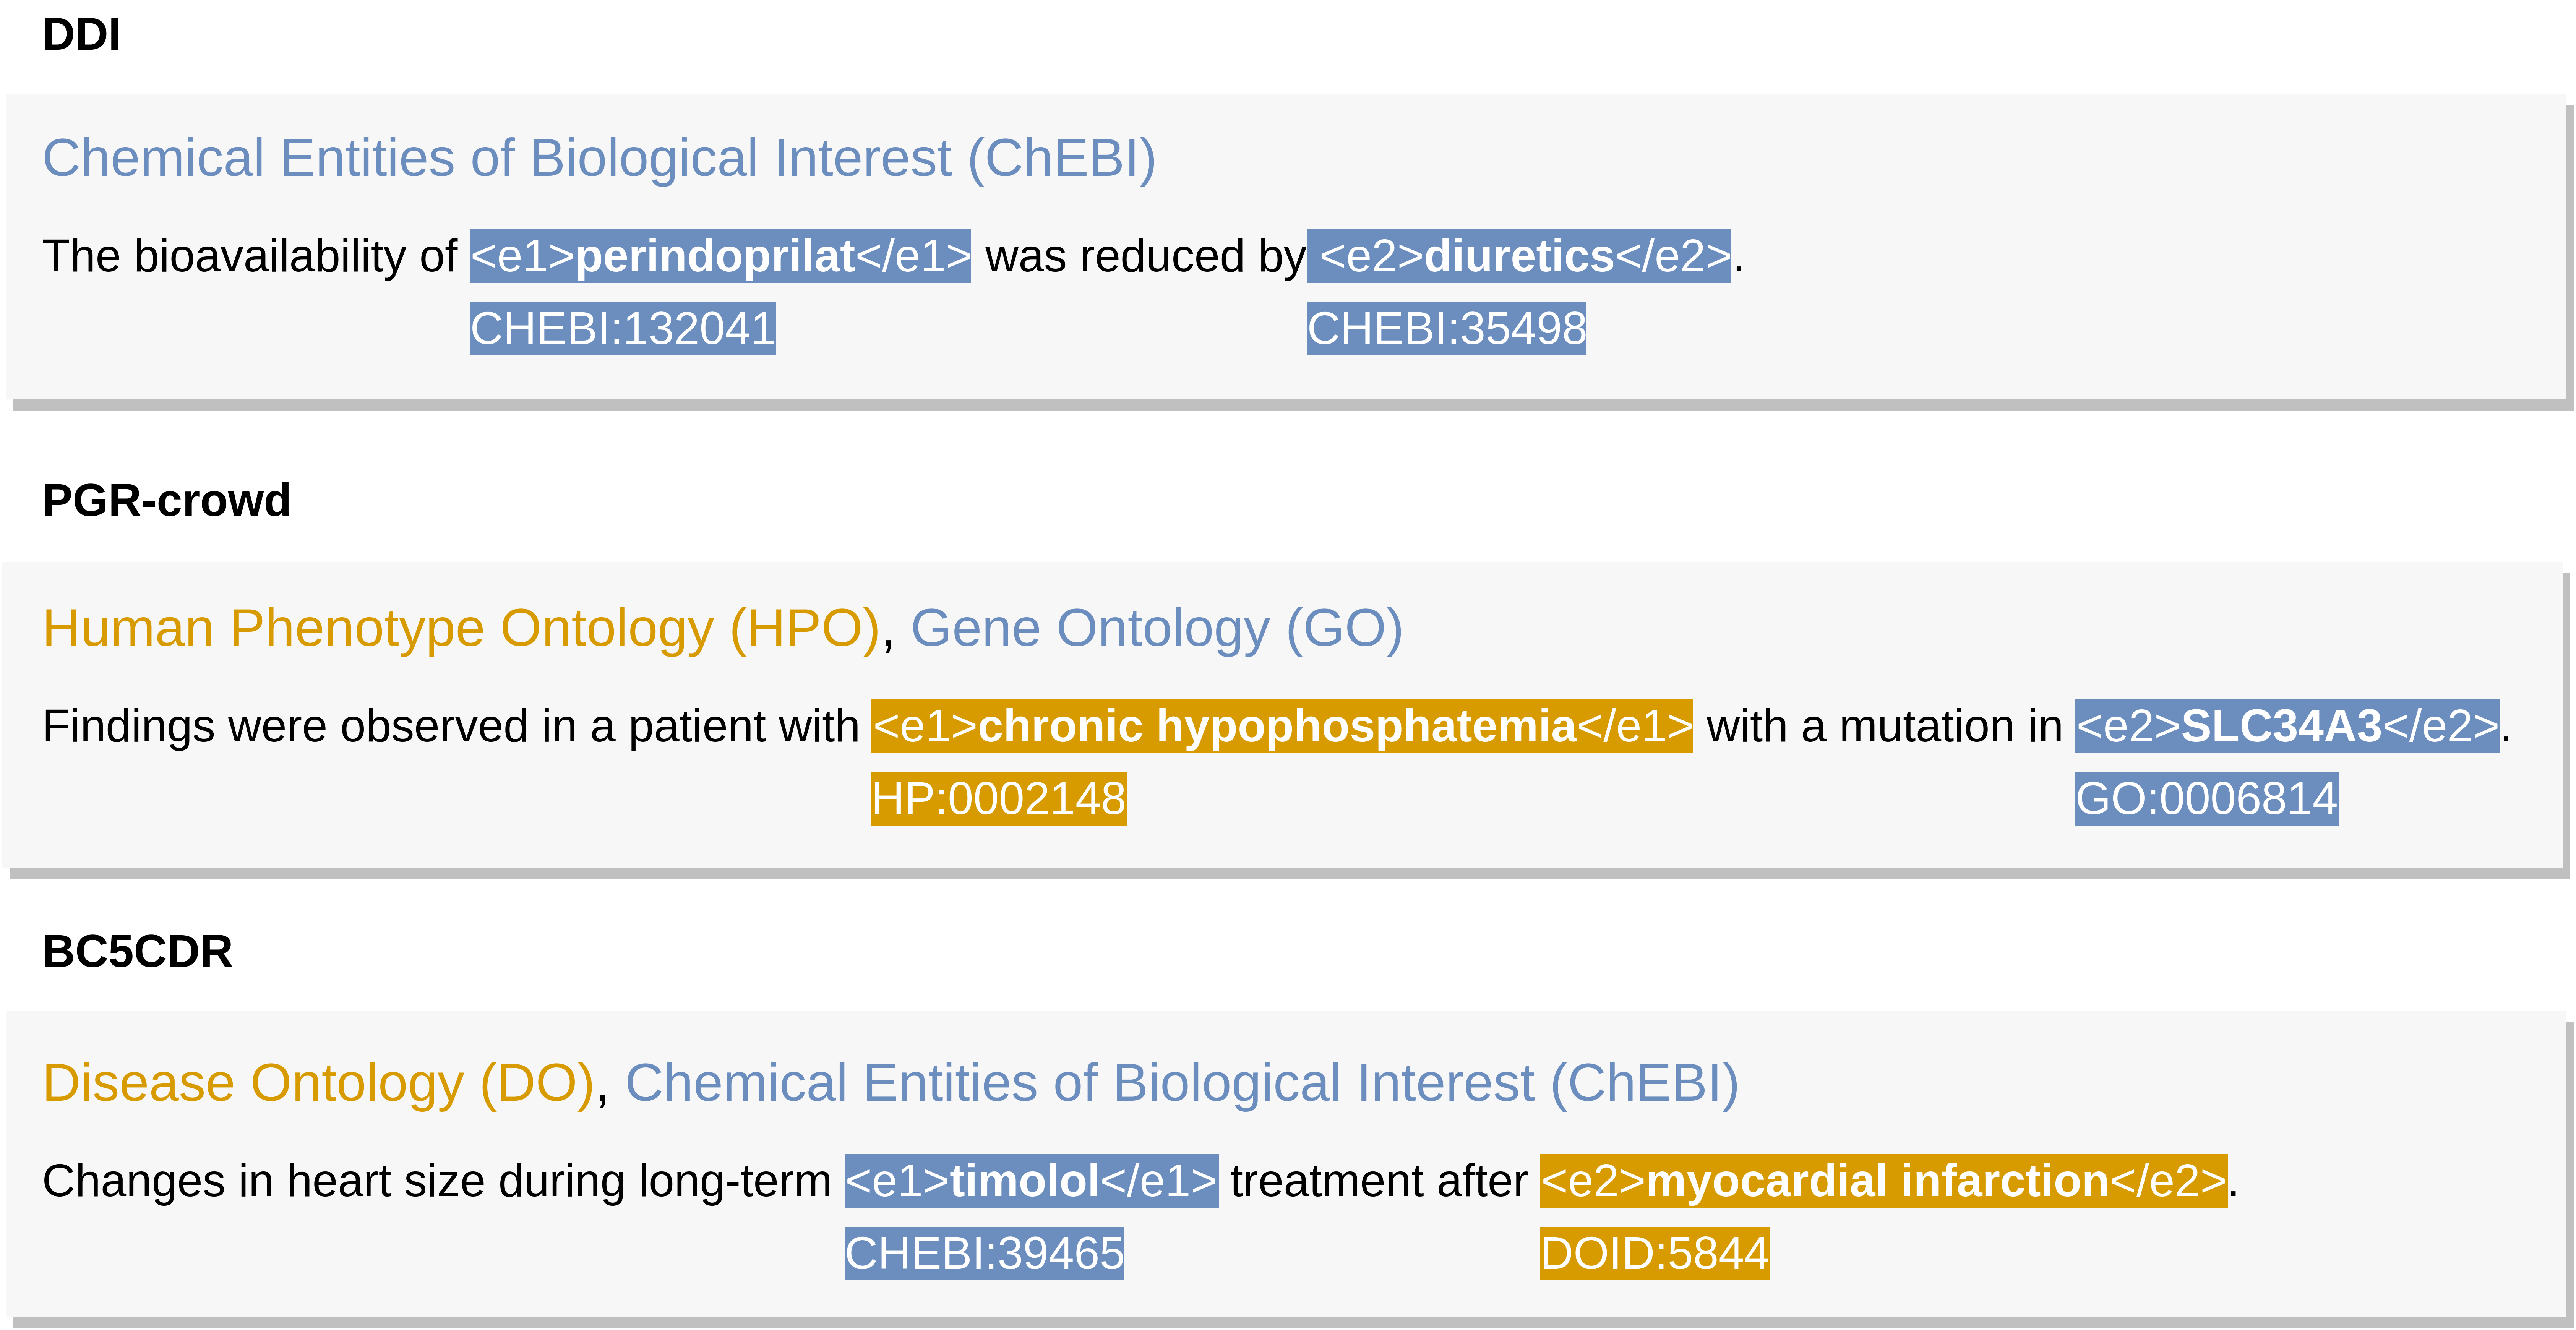
\includegraphics[width=\linewidth]{images/chapter_5/example_sentences_each_dataset.png}}
\caption[Three Sentence Examples for each dataset, DDI Corpus, PGR-crowd Corpus, and BC5CDR Corpus]{Three sentence examples for each dataset, DDI Corpus, PGR-crowd Corpus, and BC5CDR Corpus. The entities in each candidate relation are linked to corresponding knowledge bases.}\label{fig:52}
\end{figure}

We applied class weights to all datasets to normalize the different types of relations and distributions. Additionally, to train and evaluate all models on the same cross-validation splits, we split each dataset into training (60\%), validation (10\%), and test (30\%) sets. Also, our metrics presented below are displayed considering the weighted average for each type of relation to further account for the datasets' imbalances. 


\subsection{Knowledge Bases}

Several knowledge bases target biomedical entities, expanding on our information about them and their inherent relationships. Some of the knowledge bases or ontologies we can link to our target entities were mentioned above and are characterized in Table~\ref{Tab:02}\footnote{All knowledge bases were consulted on 20/04/2022}. 

\begin{table}[hbt!]
\centering
\caption[Main Characteristics of Biomedical Knowledge Bases]{The main characteristics of the following knowledge bases: Human Phenotype Ontology (HPO), Disease Ontology (DO), Chemical Entities of Biological Interest (ChEBI), and Gene Ontology (GO). All types of relations are transitive\label{Tab:02}} {\begin{tabular}{@{}lcp{3cm}p{5.5cm}@{}}\hline Knowledge bases &
Number of concepts & Type of relations & Specific characteristics\\\hline
HPO & 15670 & \textit{is-a} & Five sub-ontologies, from which \textit{phenotypic abnormality} is the most prevalent\\
DO & 13355 & \textit{is-a} & Human-specific\\
ChEBI & 153795 & \textit{is-a} & Refers to small molecular entities\\
 & & \textit{has-part} & \\
 & & \textit{is-conjugate-base-of} & \\
 & & \textit{is-conjugate-acid-of} & \\
 & & \textit{is-tautomer-of} & \\
 & & \textit{is-enantiomer-of} & \\
 & & \textit{has-functional-parent} & \\
 & & \textit{has-parent-hydride} & \\
 & & \textit{is-substituent-group-from} & \\
 & & \textit{has-role} & \\
GO & 43613 & \textit{is-a} & Three subontologies, molecular\\
 & & \textit{part-of} & function, biological process,\\
 & & \textit{has-part} & and cellular component\\
 & & \textit{regulates} & \\
 & & \textit{negatively-regulates} & \\
 & & \textit{positively-regulates} & \\\hline
\end{tabular}}
\end{table}

With few code adjustments, one can easily integrate more knowledge into K-RET in the form of other knowledge bases and has the flexibility to test different combinations swiftly.  


\subsection{Parameters and Training Details}

For each dataset, we empirically determined the best set of parameters. K-RET used a batch size of 32 for all datasets. The number of epochs ranged from 30 for DDI Corpus to 20 for PGR-crowd and BC5CDR Corpora (due to differences in dataset size). All other parameter settings were maintained from the original BERT model. The added knowledge only played a role in the fine-tuning and prediction stage.  

For the added knowledge, we varied the number of knowledge base entities allowed to link to each dataset entity in a candidate relation (or not). This variation ranged from two to five knowledge base entities per dataset entity. Our baseline represents the performance of the BERT-based systems without any added knowledge. When we refer to targeted knowledge, we mean just adding knowledge to entities in a candidate relation versus contextual knowledge, where we can add knowledge to all entities in the dataset. Figure \ref{fig:53} further elucidates the differences in the addition of knowledge. For the DDI Corpus, we used the ChEBI ontology; for the PGR-crowd, we used the HPO and the GO ontologies; and for the BC5CDR Corpus, we used the DO and ChEBI ontologies, as represented in Figure \ref{fig:52}.

\begin{figure*}[h]%figure3
\centerline{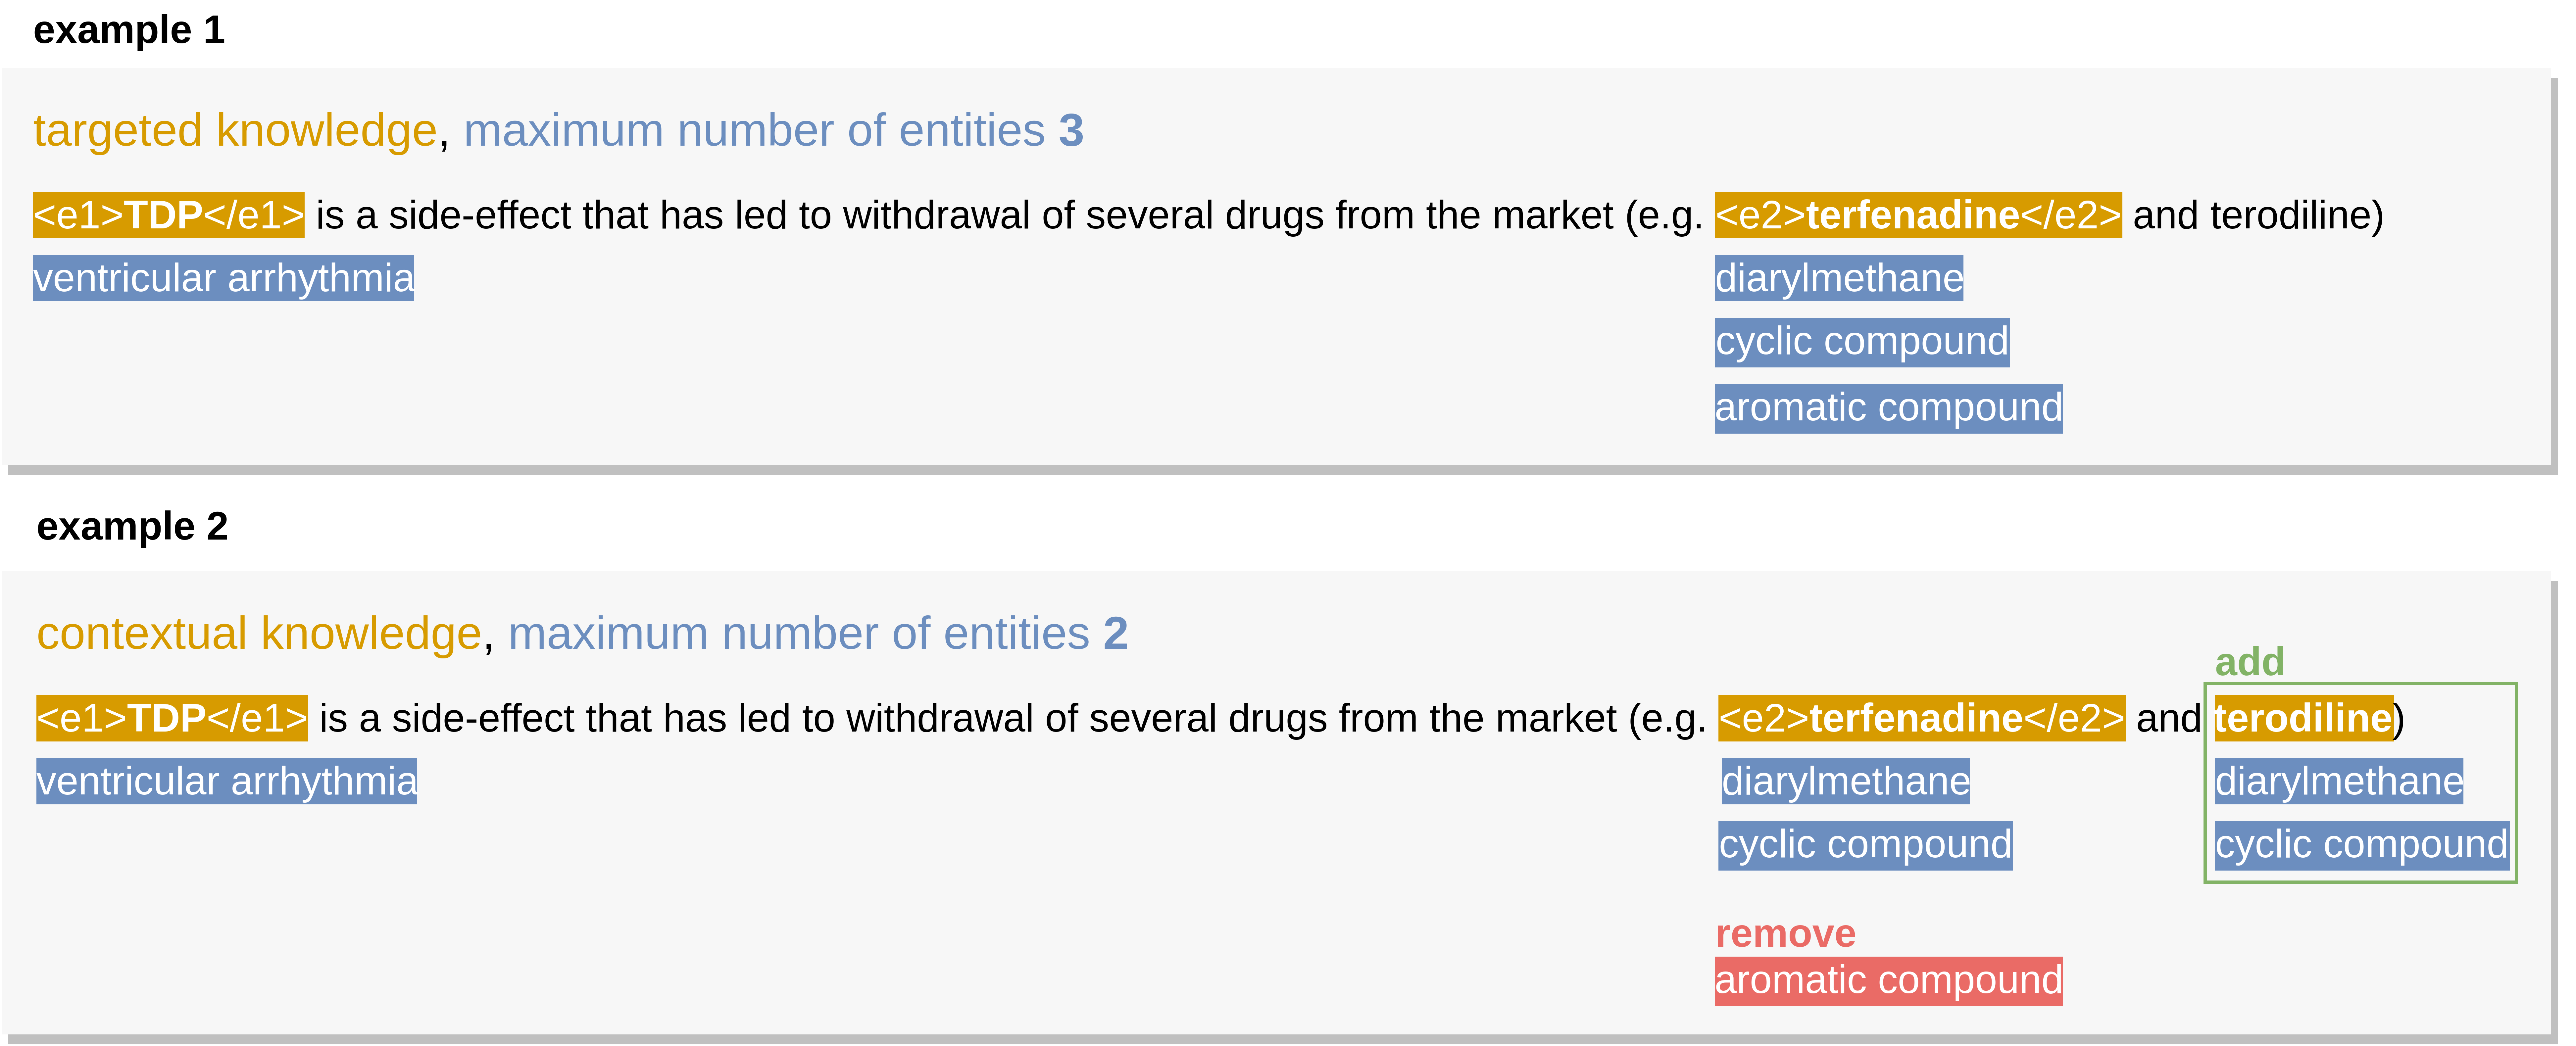
\includegraphics[width=\linewidth]{images/chapter_5/targeted_contextual_knowledge.png}}
\caption[Novelties of K-RET's Knowledge Injection Layer]{Novelties of K-RET's knowledge injection layer.  Example 1 presents a modality where we only add knowledge to entities in the candidate relation (targeted knowledge) and limit the number of knowledge base entities assigned to each entity (maximum number of entities 3). In example 2, we present the same sentence with the option of adding knowledge to all entities regardless if they are in the candidate relation (contextual knowledge) and limit the number of knowledge base entities assigned to each entity to two (maximum number of entities 2). From example 1 to example 2, we add a third knowledgeable entity (terodiline) and remove one of the knowledge base entities added (aromatic compound). The first entity can only be linked to one knowledge entity because (ventricular arrhythmia) no other association is established in the knowledge base.}\label{fig:53}
\end{figure*}

All models were trained on three Tesla M10 GPUs, taking, on average for each model, 24 hours (DDI Corpus), 1 hour (PGR-crowd Corpus), and 2 hours (BC5CDR Corpus). Each result presented in the following sections represents the averaged metrics for three runs except when it explicitly says otherwise, and each metric represents the weighted-averaged of the different labels.


\subsection{Results}

As mentioned in the previous sections, we divided our K-RET experiments into baseline, where we ran the BERT-based models without additional knowledge, targeted knowledge added to the entities in the candidate relation, and contextual knowledge added to all relevant entities in the sentence. We considered an entity relevant if present in the chosen knowledge source (i.e., a part of the domain knowledge considered). 

\subsubsection{Baseline}

To choose the best-performing BERT-based biomedical model for each of the three datasets, we used four of the most widely used systems: BERT \citep{devlin2019bert}, BioBERT \citep{lee2020biobert}, SciBERT \citep{scibert}, and PubMedBERT \citep{gu2021domain} integrated into K-BERT \citep{liu2020k} modified to perform RE. 

Table~\ref{Tab:03}\footnote{The specific models used were bert-base-uncased (BERT), scibert\_scivocab\_uncased (SciBERT), biobert-base-cased-v1.2 (BioBERT), BiomedNLP-PubMedBERT-base-uncased-abstract-fulltext (PubMedBERT)} reports the main results of testing the three datasets over the different BERT-based systems. For all three datasets, SciBERT is the best-performing system. Therefore, in our following experiments, we used SciBERT as the baseline system to which we added a knowledge layer.  

\begin{table}[h]
\centering
\caption[Baseline Performance of the Four Models for Each Dataset]{The baseline performance of the four models for each dataset\label{Tab:03}} 
\begin{tabular}{@{}llcccc@{}}\hline
Dataset & Model & Precision & Recall & F-measure & Accuracy\\\hline
PGR-crowd & BERT & 0.7247 & 0.7766 & 0.7332 & 0.7765\\
& SciBERT & \textbf{0.7680} & \textbf{0.8002} & \textbf{0.7462} & \textbf{0.7999}\\
& BioBERT & 0.6224 & 0.7888 & 0.6957 & 0.7888\\
& PubMedBERT & 0.7201 & 0.7834 & 0.7191 & 0.7833\\\hline
DDI & BERT & 0.7764 & 0.7798 & 0.7775 & 0.7796\\
& SciBERT & \textbf{0.7906} & \textbf{0.7964} & \textbf{0.7930} & \textbf{0.7960}\\
& BioBERT & 0.7796 & 0.7648 & 0.7680 & 0.7647\\
& PubMedBERT & 0.7801 & 0.7227 & 0.7473 & 0.7227\\\hline
BC5CDR & BERT & 0.5804 & 0.5614 & 0.5670 & 0.5615\\
& SciBERT & \textbf{0.6266} & \textbf{0.6364} & \textbf{0.6289} & \textbf{0.6363}\\
& BioBERT & 0.6150 & 0.6132 & 0.6142 & 0.6131\\
& PubMedBERT & 0.6091 & 0.6218 & 0.6113 & 0.6217\\\hline
\end{tabular}
\end{table}


\subsubsection{Targeted Knowledge}

For targeted knowledge, we added from two to five knowledge base entities to each entity in the candidate relation, as shown previously in example 1 (Figure \ref{fig:53}). Although we define the number of knowledge base entities to add, we are always limited by how many entities each entity is linked to in the knowledge base itself. Figure \ref{fig:54} presents the performance of the three datasets from no added knowledge (baseline) to five added entities per entity in the candidate relation.

Figure \ref{fig:54} shows that none of the K-RET models trained performs better than the baseline at any number of knowledge base added entities. For all datasets, there is a slight decrease in performance, with the BC5CDR Corpus having a small increase in performance when the number of added knowledge base entities equals three.  

\begin{figure}[H]
\centering
\begin{minipage}{0.48\textwidth}
\centering
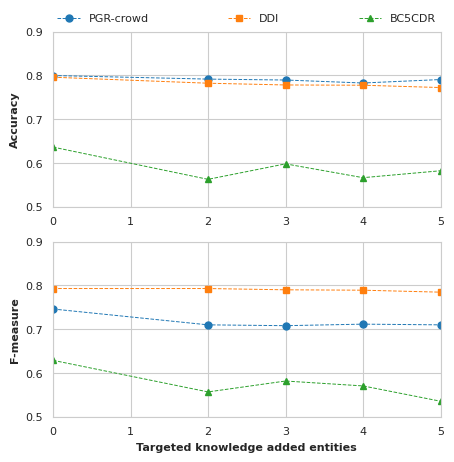
\includegraphics[width=0.97\linewidth]{images/chapter_5/tk.png}
\caption[K-RET Performance of the Targeted Knowledge Configuration]{The performance of the targeted knowledge K-RET configuration for the three datasets in Accuracy and F-Measure (top and bottom graphs, respectively) regarding the different number of added knowledge base entities.}\label{fig:54}
\end{minipage}
\hfill
\begin{minipage}{0.48\textwidth}
\centering
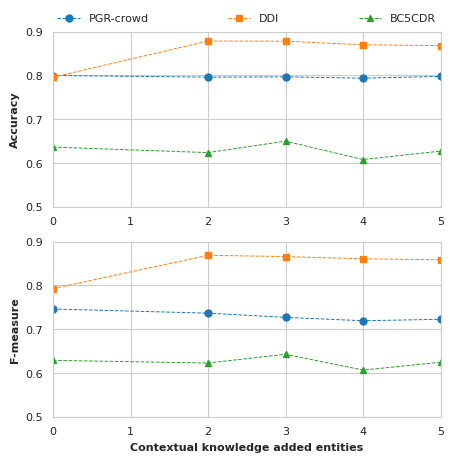
\includegraphics[width=0.97\linewidth]{images/chapter_5/ck.png}
\caption[K-RET Performance of the Contextual Knowledge Configuration]{The performance of the contextual knowledge K-RET configuration for the three datasets in Accuracy and F-Measure (top and bottom graphs, respectively) regarding the different number of added knowledge base entities.}\label{fig:55}
\end{minipage}
\end{figure}

\subsubsection{Contextual Knowledge}

We followed the same configuration mentioned above for contextual knowledge from two to five knowledge base entities added to each relevant entity in the sentence. Figure \ref{fig:55} presents the performance of the three datasets from no added knowledge (baseline) to five added entities per relevant entity. 

Figure \ref{fig:55} shows a performance increase from baseline to K-RET on the DDI and BC5CDR Corpora. For the PGR-crowd Corpus, while the performance is better than for targeted knowledge, the baseline performance still outperforms K-RET. Similarly, the BC5CDR's best performance is when the number of added knowledge base entities equals three, but this time surpasses the baseline. 

\vspace{10pt}
 
Table~\ref{Tab:04}\footnote{To facilitate table readability, we omitted the Standard Deviation (SD) values that range from 0.005 to 0.029 across all datasets due to the low impact these have on the interpretation of the final results.} presents the best results for each main model configuration (targeted and contextual), including the contextual knowledge configuration over ten runs to determine the statistical significance of the best configuration accurately and the corresponding baseline considered previously and regarding the majority label. The baseline\textsubscript{ML} represents the results if we assign the same label (majority label) to all the test relations. 

The results show that the contextual knowledge configuration over three runs prevails as the best model in two datasets (DDI and BC5CDR), with the targeted knowledge configuration not surpassing the baseline for any dataset. However, the BC5CDR Corpus presents a p-value of 0.8108 for F-measure and 0.8681 for accuracy ($\alpha = 0.05$), demonstrating a lack of significant difference between the means of Baseline and CK-RET\textsubscript{10}. Nonetheless, the DDI Corpus presents a p-value of $2.91 \times 10^{-12}$ for F-measure and $1.44 \times 10^{-12}$ for accuracy ($\alpha = 0.05$), validating a significant difference between the means of Baseline and CK-RET\textsubscript{10}. The p-values were determined using a one-tailed $t$-test.  

\begin{table}[h]
\centering
\caption[Final K-RET Performance Results]{The final K-RET performance results. The best-performing models for each dataset concerning baseline considering the majority label, baseline, targeted knowledge, contextual knowledge, and contextual knowledge over ten runs\label{Tab:04}} 
\begin{tabular}{@{}llcccc@{}}\hline
Dataset & Model & Precision & Recall & F-measure & Accuracy\\\hline
PGR-crowd & Baseline\textsubscript{ML} & 0.6222 & 0.7888 & 0.6957 & 0.7888\\
& Baseline & \textbf{0.7680} & \textbf{0.8002} & \textbf{0.7462} & \textbf{0.7999}\\
& TK-RET & 0.7891 & 0.7914 & 0.7100 & 0.7917\\
& CK-RET & 0.7614 & 0.7960 & 0.7367 & 0.7962\\\cline{2-6}

& CK-RET\textsubscript{10} & 0.7441 & 0.7933 & 0.7206 & 0.7934\\
\hline

DDI & Baseline\textsubscript{ML} & 0.7267 & 0.8525 & 0.7846 & 0.8525\\
& Baseline & 0.7906 & 0.7964 & 0.7930 & 0.7960\\
& TK-RET & 0.8132 & 0.7820 & 0.7930 & 0.7823\\
& CK-RET & 0.8674 & 0.8791 & 0.8690 & 0.8788\\\cline{2-6}

& CK-RET\textsubscript{10} & \textbf{0.8704} & \textbf{0.8805} & \textbf{0.8719} & \textbf{0.8804} \\\hline

BC5CDR & Baseline\textsubscript{ML} & 0.3803 & 0.6167 & 0.4705 & 0.6167\\
 & Baseline & 0.6266 & 0.6364 & 0.6289 & 0.6363\\
& TK-RET & 0.5838 & 0.5977 & 0.5816 & 0.5980\\
& CK-RET & \textbf{0.6412} & \textbf{0.6499} & \textbf{0.6428} & \textbf{0.6498}\\\cline{2-6}

\rule{0pt}{3.2ex} & CK-RET\textsubscript{10} & 0.6317 & 0.6348 & 0.6309 & 0.6347 \\\hline
\end{tabular}
\end{table}

Table~\ref{Tab:05} reflects the specific performance of the DDI Corpus per type of relation (\textit{effect}, \textit{advice}, \textit{mechanism}, \textit{int}, and \textit{false}) for each main model configuration. Table A1 and Table A2 in Supplementary Data present the same results for PGR-crowd and BC5CDR Corpora. For the DDI Corpus, we also performed ablation regarding multi-token entities by limiting the association of knowledge to the first entity within the multi-token considered. We obtained an F-measure of 0.8663 and an accuracy of 0.8732.    

\begin{table}[h]
\centering
\caption[DDI Corpus Performance per Type of Relation]{DDI Corpus performance per type of relation\label{Tab:05}} 
\begin{tabular}{@{}llccccc@{}}
\hline \multirow{2}{*}{Metrics} & \multirow{2}{*}{Model} &
\multicolumn{5}{c}{Type} \\\cline{3-7}
& & Effect & Advice & Mechanism & Int & False\\\hline
Precision & Baseline & 0.1770 & 0.0890 & 0.2720 & 0.2800 & 0.8060\\
& TK-RET & 0.2747 & 0.3053 & 0.3623 & 0.2360 & 0.9020 \\
& CK-RET & 0.5137 & \textbf{0.6720} & \textbf{0.5757} & 0.5963 & 0.9163 \\\cline{2-7}

& CK-RET\textsubscript{10} & \textbf{0.5524} & 0.6370 & 0.5411 & \textbf{0.6659} & \textbf{0.9194} \\
\hline
Recall & Baseline & 0.2000 & 0.0730 & 0.1810 & 0.3850 & 0.9040\\
& TK-RET & 0.4677 & 0.3490 & 0.5127 & 0.0160 & 0.8487 \\
& CK-RET & 0.4533 & 0.2937 & 0.4950 & \textbf{0.4340} & \textbf{0.9600} \\\cline{2-7}

& CK-RET\textsubscript{10} & \textbf{0.4758} & \textbf{0.3226} & \textbf{0.5318} & 0.3946 & 0.9579\\
\hline
F-measure & Baseline & 0.1880 & 0.0800 & 0.2170 & 0.3250 & 0.9000\\
& TK-RET & 0.3423 & 0.3240 & 0.4187 & 0.0293 & 0.8743 \\
& CK-RET & 0.4810 & 0.4077 & 0.5317 & \textbf{0.5017} & 0.9377 \\\cline{2-7}

& CK-RET\textsubscript{10} & \textbf{0.5099} & \textbf{0.4266} & \textbf{0.5329} & 0.4924 & \textbf{0.9384}\\
\hline
\end{tabular}
\end{table}


\section{Discussion}

From the experiences conducted throughout the previous section, we can infer that adding knowledge can significantly improve the state-of-the-art performance of one of the most used biomedical Relation Extraction (RE) datasets, mainly when using contextual knowledge. However, there is a difference in how significantly we can improve performance, from nothing (PGR-crowd Corpus) to over 0.076 percentage points (DDI Corpus). Several factors can explain the differences in performance for the different datasets, such as dataset size and label distribution, knowledge base size and coverage of the dataset entities, or the average number of knowledge base entities that can be linked to each dataset entity.

For the PGR-crowd Corpus, while all entities are linked to one of two knowledge bases, the Human Phenotype Ontology (HPO) or the Gene Ontology (GO), the linking to the GO is already second-handed. In the PGR-crowd Corpus, the authors recognized gene entities and posteriorly linked them to their most representative GO term. We do not use their gene identifiers directly because these biomedical entities are not directly represented in any hierarchic knowledge base. Thus, we used the GO terms to add further information and, consequently, distanced ourselves from the original gene entity. However, what made the most significant impact in the lack of increase in performance is the distribution of labels being predominantly \textit{true}. Identifying undetected \textit{true} relations is more challenging than if the dataset was more balanced (e.g., the BC5CDR Corpus) or with the inverse distribution (e.g., the DDI Corpus). Also, for the specific case of PGR-crowd Corpus, there could be ambiguity if an acronym describes a human phenotype or a gene since these can often overlap. This ambiguity is an open problem, and in this work, we opted not to consider human phenotype entities acronyms for contextual knowledge, which could be made us lose valuable information.   

With the BC5CDR Corpus, K-RET only surpassed the baseline when adding contextual knowledge by slightly over 1\% in both F-measure and accuracy and was unsuccessful at demonstrating a significant difference between the baseline and the best-performing configuration. Although the impact on performance is not preeminent, the fact that this dataset is denser in the number of relevant entities per sentence and more evenly distributed than the PGR-crowd Corpus increases the impact of the addition of knowledge. This behaviour occurs when knowledge is added directly to the candidate relation's target entities and peripherally to other relevant entities. 

The DDI Corpus is unbalanced in favour of \textit{no\_relation}/\textit{false} labels. Therefore, finding \textit{true} relations is more challenging. This dataset's distribution of labels is ideal for increasing the impact of adding knowledge. The label distribution, the highly dense text in relevant entities, and the ampler size of the knowledge base used, Chemical Entities of Biological Interest (ChEBI), all contribute to the rise in performance by adding contextual knowledge. The improvements from baseline were 7.60\% for contextual knowledge in F-measure. We also verified that adding knowledge made a bigger impact on system performance than using multi-token entities by contributing to an average improvement of 0.0704 data points in F-measure and 0.0756 in accuracy. 

K-RET was able to design a more efficient and flexible knowledge layer than the previous attempt in the work of \cite{liu2020k} by applying knowledge injection to the biomedical RE task. First, by proving the utility of contextualizing tokens, with substantial improvements in one of the three datasets described above from targeted to contextual token usage. Second, by the possibility of adding more than one knowledge source to cover the domains of all relevant entities mentioned in the training data. Third, by incorporating the option of adding knowledge to multi-token entities instead of only single-token. We determined experimentally for the DDI Corpus the multi-token approach to be more thorough, which can be explained by those entities constituting the majority of biomedical entities described in the datasets used for testing.

\section{Conclusion}

This paper proposed a new biomedical Relation Extraction (RE) system, K-RET, that incorporates knowledge in the form of ontologies into BERT-based systems to enrich and complement the data used for training. K-RET is a flexible system that can handle different associations, integrate knowledge from multiple sources, define where to apply the knowledge, and deal with multi-token entities. We used three independent and open-access RE datasets to test our system concerning different types of biomedical entities with different characteristics (i.e., label distribution). Allied with the three datasets, we used four knowledge bases to inject knowledge according to the type of entities involved in the candidate relations. The best-performing dataset was the DDI Corpus allied with the Chemical Entities of Biological Interest (ChEBI) knowledge base, with significant average improvements compared with the baseline in the order of 7.60\% and 8.28\% for F-measure and accuracy, respectively. For the BC5CDR Corpus, we also had modest improvements (an average of 1.39\% and 1.35\% for F-measure and accuracy), even though we did not find these results significant. Differently, for the PGR-crowd Corpus, there was no significant change in performance from the addition of knowledge. Thus, we concluded that the label distribution and relevant entity density within the training data significantly affect how our system performs. Nevertheless, we successfully demonstrated the power of adding external knowledge to training data and how to accommodate it to different domain data. 

In a nutshell, the K-RET system successfully added contextual knowledge, more than one knowledge source, and knowledge to multi-token entities. 

For future work, we would like to explore the impact of different knowledge bases and combinations within the ones we already used. Also, we would like to analyze further and examine the implications of peripherical contextual entities on assigning a label for a candidate relation and entities overlapping within different knowledge bases. 


\hypertarget{6}{}

\rhead{A Hybrid Approach toward Biomedical Relation Extraction Training Corpora}
\lhead{Chapter 6}

\chapter[A Hybrid Approach toward Biomedical Relation Extraction Training Corpora: Combining Distant Supervision with Crowdsourcing]
{\huge A Hybrid Approach toward Biomedical Relation Extraction Training Corpora: Combining Distant Supervision with Crowdsourcing \\
\Large \textmd{Diana Sousa, Andre Lamurias, and Francisco M. Couto}}

\vspace{-1.6cm}

% Gray Line
\begingroup
\color{black}
\par\noindent\rule{\textwidth}{0.4pt}
\endgroup

\noindent{This chapter tackles Objective 2 by demonstrating the possibility of creating \acl{RE} (RE) training data using distant supervision allied with crowdsourcing and corresponds to the journal article:} 

\begin{itemize}[label=]
    \item{\textbf{Sousa, D.}, Lamurias, A., and Couto, F. M. (2020). \textbf{A Hybrid Approach Toward Biomedical Relation Extraction Training Corpora: Combining Distant Supervision with Crowdsourcing}. Database, 2020:1-15. (Q1 Scimago) \citep{sousa2020hybrid}} 
\end{itemize}

\noindent{\textbf{Abstract.} Biomedical RE datasets are vital in the construction of knowledge bases and potentiate the discovery of new interactions. There are several ways to create biomedical RE datasets, some more reliable than others, such as using domain expert annotations. However, the emerging use of crowdsourcing platforms, such as Amazon Mechanical Turk (MTurk), can potentially reduce the cost of RE dataset construction, even if the same level of quality cannot be guaranteed. There is a lack of power for the researcher to control who, how and in what context workers engage in crowdsourcing platforms. Hence, allying distant supervision with crowdsourcing can be a more reliable alternative. The crowdsourcing workers would be asked only to rectify or discard already existing annotations, making the process less dependent on their ability to interpret complex biomedical sentences. In this work, we use a previously created distantly supervised human phenotype–gene relations (PGR) dataset to perform crowdsourcing validation. We divided the original dataset into two annotation tasks: Task 1, 70\% of the dataset annotated by one worker, and Task 2, 30\% of the dataset annotated by seven workers. Also, for Task 2, we added an extra rater on-site and a domain expert to further assess the crowdsourcing validation quality. Here, we describe a detailed pipeline for RE crowdsourcing validation, create a new release of the PGR dataset with partial domain expert revision, and assess the quality of the MTurk platform. We applied the new dataset to two state-of-the-art deep learning systems (BiOnt and BioBERT) and compared its performance with the original PGR dataset, as well as combinations between the two, achieving a 0.3494 increase in average F-measure. The code supporting our work and the new release of the PGR dataset is available at \url{https://github.com/lasigeBioTM/PGR-crowd.}}


\section{Introduction}

Knowledge bases play a fundamental role in the way we store, organize and retrieve information. More specifically, biological knowledge bases are commonplace for researchers and clinicians to access all types of biomedical data retrieved from biomedical literature \citep{arnaboldi2020text}. Previous works annotated biomedical literature by resorting to domain expert annotators \citep{herrero2013ddi}, crowdsourcing platforms \citep{tsueng2020applying}, or distantly supervised techniques \citep{sousa2019silver}. The main aim of these researchers is to tackle the lack of annotated datasets for biomedical information extraction systems. However, when applying distantly supervised techniques, the annotations are not as reliable as when done by domain experts, and it still needs to be adequately reviewed before the extracted information can be added to any biomedical repository. Hence, the added advantage of automating the extraction of information using distant supervision is slightly impaired by the need to review it, which is not only costly but time and resource-consuming.  Moreover, when targeting Relation Extraction (RE) between entities of different domains or document summarization tasks \citep{narayan2018ranking}, the revision process becomes cumbersome when compared to other information extraction tasks, given its higher complexity that normally requires knowledge of multiple domains. 

The alternative way to create reliable gold standard datasets that do not resort to domain expert curation could be allying distant supervision with crowdsourcing \citep{gormley2010non,liu2016effective,collovini2018annotating}. Before integrating data extracted from distant supervision pipelines into biological knowledge bases or using it as training data for biomedical information extraction systems, the data would go through a confirmation or review phase in the form of crowdsourcing. Crowdsourcing platforms are becoming increasingly popular to address the problem of lack of training corpora for natural language processing (NLP) tasks \citep{callison2010creating}. Currently, the most popular platform for this purpose is Amazon Mechanical Turk (MTurk) \citep{ipeirotis2010quality,yetisgen2010preliminary,khare2015scaling}. Some platforms created a trust layer over MTurk to facilitate task specification and monitoring \citep{wang2013perspectives}, such as Figure Eight (previously known as CrowdFlower) \citep{li2016crowdsourcing,feyisetan2015towards}, which is widely used by researchers for biomedical NLP related tasks. 

One of the problems of using crowdsourcing platforms is the lack of domain expertise. While most platforms allow us to specify some criteria (e.g., degree of education) in exchange for an increased price per task, it is not feasible to specify expertise in particular biomedical domains. Not only that, but there is no guarantee that the quality promised is the quality provided because some malicious workers often take advantage of the difficulty in implementing a verification procedure and submit answers of low quality \citep{callison2010creating}. Task redundancy can be a solution, but it also increases the costs of using crowdsourcing approaches, partially defeating the purpose of these platforms. The question should be whether the quality of the workers is good enough for the purpose of the task and if the difference in quality when compared to domain experts is compensated by the decrease in costs. In the case of the MTurk platform, some studies have supported its suitability for various tasks \citep{mortensen2018comparing}. However, it fails in transparency about its workers' context (e.g., background), if MTurk constitutes their primary form of income or not, what is their motivation for completing the tasks, and if this introduces bias to the tasks at hand. These and other ethical questions have been discussed in depth by some researchers \citep{fort2011amazon,paolacci2014inside}.

In this work, we leveraged an existing dataset of biomedical relations created through distant supervision and submitted it to the MTurk platform for crowdsourcing validation. With the exhaustive review of the performance of the original and new datasets, we assessed the viability of combining distant supervision and crowdsourcing for the field of biomedical RE. 

Our work used an open-source dataset, the PGR dataset \citep{sousa2019silver}, based on distant supervision, that features both human phenotype and gene annotations and their relations. Since it is a silver standard dataset, it has not been reviewed by domain experts, leading to wrongly labelled relations and other errors. These errors can be from Named-Entity Recognition (NER) (e.g., acronyms of diseases annotated as genes), which was also done automatically, or sentence format errors. To rectify these errors, we used the MTurk platform to validate, alter, or discard the relations within the PGR dataset. We achieved this by dividing the original dataset into two partitions, one of 70\% (Task 1), where each relation was rated by one Amazon worker, and another of 30\% (Task 2), where each relation was rated by seven distinct workers. We validated our approach through inter-rater agreement using the Fleiss’ kappa \citep{mchugh2012interrater} and the  Krippendorff’s alpha \citep{krippendorff2011computing} metrics for Task 2. Further, we also provided the 30\% partition of the PGR dataset used for Task 2 to an external rater (on-site, without previous curating experience but holding a Biochemistry degree) and to a domain expert (with previous curating experience, holding a PhD in Bioinformatics). These different levels of expertise enlightened the difficulties of curating the dataset and the limitations associated with each level. To evaluate and compare the quality of the crowdsourced Amazon dataset, we applied it to two state-of-the-art deep learning systems and compared its performance with the original PGR dataset, as well as combinations between the two. The deep learning systems used were BiOnt \citep{sousa2020biont} and BioBERT \citep{lee2020biobert}, that feature relation extraction between different biomedical entities with high performance, and, in the case of BiOnt, it was already used in conjunction with the PGR dataset. 

The performance of the MTurk workers in comparison with our on-site curator and the domain expert was generally good for accessing NER or sentence format errors (approximately 16\% of relations). However, the MTurk workers struggle to identify false relations (separate entities without association in a sentence). The struggle to identify these relations can be due to the complexity of the sentences or quality issues related to the MTurk platform validation of workers, which we will discuss in more detail in the following sections. Further, the inter-rater agreement for Task 2 showed a slight to a fair agreement (about 0.20-0.21), which is below what we expected and we believe could be related to the problems of sentence complexity and quality reported.  Regarding the performance of the crowdsourced Amazon dataset in the application of the BiOnt and BioBERT systems, we had an average increase of 0.3494 in F-measure, taking into account all the experiences concerning the original PGR dataset. 
 
The main takeaways of this work were the need for further validation of the use of crowdsourcing platforms, such as the MTurk platform, and the potential of using distant supervision allied with crowdsourcing to produce gold standard datasets with which we can train viable models and detect relevant biomedical relations. This work resulted in the following contributions:

\begin{itemize}
    \item Pipeline for RE crowdsourcing, in which we describe in detail all the base concepts and steps taken to produce the new crowdsourced dataset.
    \item New release of the PGR Dataset, which will be made freely available to the community.
    \item Assessment of the quality of results obtained with the MTurk platform (through statistical analysis and direct comparison with on-site rater and domain expert).
\end{itemize}

\section{Materials and Methods}

This section presents an overview of the PGR dataset \citep{sousa2019silver}, a brief presentation of the Amazon Mechanical Turk (MTurk) platform, and the integration of the dataset into the MTurk platform (including the design, configuration, and evaluation stages). We now describe how we proceeded with each of these stages: 

\begin{enumerate}
    \item Design
    \begin{enumerate}
        \item Set up the tasks (Human Intelligence Task - HIT) to be simple to understand and easy to accomplish by the employees (i.e., workers or turkers).
        \item Define the guidelines (instructions) with examples for the workers to better understand the presented HITs. 
    \end{enumerate}
    \item Configuration
    \begin{enumerate}
        \item Configure the MTurk platform specifying different criteria (for workers) and wages (i.e., reward).
        \item Submit the HITs within the platform.
    \end{enumerate}
    \item Evaluation
    \begin{enumerate}
        \item Calculate inter-rater agreement.
        \item Compare  the PGR dataset before and after MTurk crowdsourcing assessment by employing  two different deep learning models (BiOnt \citep{sousa2020biont} and BioBERT \citep{lee2020biobert}).
    \end{enumerate}
\end{enumerate}

An overview of the pipeline of the work described in this paper can be found in Figure \ref{fig61}.

\begin{figure}
\centering
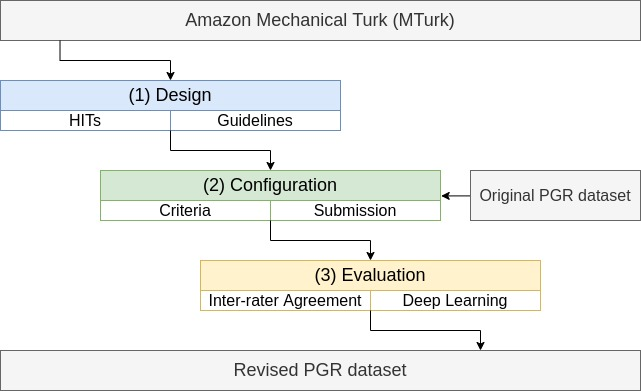
\includegraphics[width=0.8\linewidth]{images/chapter_6/figure_1.jpg}
\caption[Pipeline to Incorporate the PGR Dataset into MTurk]{The pipeline to incorporate the PGR dataset into the Amazon Mechanical Turk (MTurk) platform, including the design, configuration, and evaluation stages.} \label{fig61}
\end{figure}

\subsection{PGR Dataset}

The PGR dataset is a silver standard corpus of PubMed abstracts featuring human phenotype and gene annotations and their relations \citep{sousa2019silver}. In this dataset, all the annotations were generated in a fully automated fashion (silver standard), taking a distant supervision approach, opposite to a manually annotated dataset where domain experts generate the annotations (gold standard). 

The first release of the  PGR dataset focused mostly on the initial release of the dataset (10/12/2018), where a small subset of relations (6\%) was manually reviewed to evaluate the PGR dataset quality and also to use as a test corpus for machine learning model evaluation. The second release (11/03/2019) captured a more clear-cut search of the type of abstracts to retrieve, such as abstracts regarding diseases, their associated phenotypes and genes, increasing from about 2.5 relations per abstract to about 3.0 relations per abstract, and the overall number of relations by 2-fold. In this work, we are going to use the second release of the PGR dataset to generate an improved third release. 

The relations identified in the PGR dataset are either Known if present in the knowledge base of relations provided by the Human Phenotype Ontology (HPO) group \citep{kohler2017human} or Unknown otherwise. Table \ref{tab1} presents the numbers for the second release of the PGR dataset.

\begin{table}[h]
\centering
\caption[General Statistics for the PGR Dataset]{The number of abstracts, phenotype and gene annotations, and of known, unknown and total of relations for the second release (11/03/2019) of the PGR dataset (partial table from \citep{sousa2019silver})}\label{tab1}
\begin{tabular}{cccccc}
\hline
\multirow{2}{*}{Abstracts} & \multicolumn{2}{c}{Annotations} & \multicolumn{3}{c}{Relations} \\
\cline{2-6}
& Phenotype & Gene & Known & Unknown & Total \\
\hline
2657 & 9553 & 23786 & 2480 & 5483 & 7963 \\
\hline
\end{tabular}
\end{table}

\subsection{Amazon Mechanical Turk}

The Amazon Mechanical Turk (MTurk) is a crowdsourcing web service (marketplace) that facilitates the use of human intelligence by individuals and businesses that are in demand to complete specific tasks \citep{paolacci2010running}. In this web service, the employees (i.e., workers or turkers) execute tasks (i.e., HITs) submitted by employers (i.e., requesters) to earn a predefined wage (i.e., reward). The type of HITs that MTurk allows requesters to submit ranges from sentiment analysis and document classification in the language domain to image classification in the vision domain. Requesters post HITs to workers who meet their specified criteria (e.g., degree of education) and predefined both a reward and maximum time allotted for completing each task. Both requesters and workers remain anonymous throughout the process (workers can be identified through an internal identifier provided by Amazon). 

The three main benefits of the MTurk platform are: (1) optimized efficiency by allowing requesters to outsource tasks that need to be handled manually but do not require the requester or their employees' expertise; (2) increased flexibility for requesters to quickly scale their businesses without needing to scale their in-house workforce, and (3) cost reduction by eliminating the need for requesters to employ a temporary workforce and all the management costs associated with it \citep{ipeirotis2010quality}.

Some previous works using MTurk in the biomedical field include named-entity recognition and curation of biomedical entities labels’. \cite{yetisgen2010preliminary} used MTurk to extract named entities, such as medical conditions, medication, and laboratory tests, from clinical trial descriptions. \cite{good2014microtask} used it for disease mention annotation in PubMed abstracts. Similarly to our approach, \cite{khare2015scaling} used MTurk to curate indications from drug labels, i.e., to judge whether a drug is used in managing a highlighted disease.

\subsection{Integration into Amazon Mechanical Turk Platform}

The MTurk platform provides a wide range of customizable templates to start a new project. The template closest to our previously described curation task was the Document Classification template within the Language field that we leveraged to set up our PGR HITs. To facilitate the evaluation of the workers' performance, we divided the original dataset into partitions of 70\% (Task 1), where each relation was rated by one Amazon worker and 30\% (Task 2), where each relation was rated seven times by seven distinct workers. We also had to define guidelines (instructions) with examples for the workers to understand the task at hand thoroughly. Further, each project required defining criteria to select the workers that better suited the goals of the project and determining the reward per HIT for each worker before submission. Finally, after receiving the results (which took about two weeks), we had to evaluate the performance of our workers. The evaluation was done by calculating the inter-rater agreement and by comparing the performance of the PGR dataset before and after curation with existing deep learning tools.  

We describe the detailed steps that we took and the reasoning for each decision made in the following sections. 

\subsubsection{Design}

\paragraph{HITs}

As stated previously, we adapted the Document Classification template to set up our HITs. Thus, the workers were presented with a sentence with two entities in bold (the human phenotype and the gene entities) and a set of three possible classifications (true relation, false relation, or wrongly labelled relations due to errors in the NER stage or wrong sentence format). Figure \ref{fig2} represents an example of a HIT as presented to the workers (Task 2).

\begin{figure}
\centering
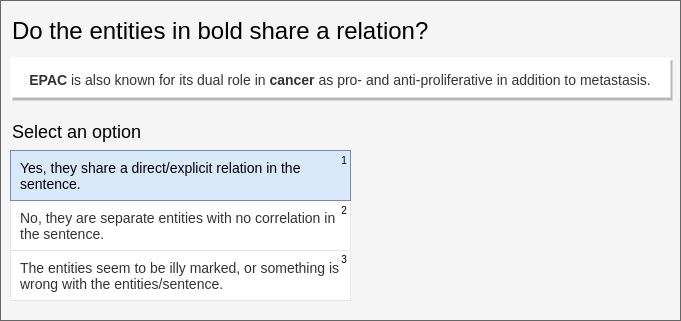
\includegraphics[width=0.8\linewidth]{images/chapter_6/figure_2.jpg}
\caption[HIT Example]{An example of a HIT presented to the workers and the available options.} \label{fig2}
\end{figure}

\paragraph{Guidelines}

In this work, we considered that rather than defining strict guidelines, it would be more intuitive for the workers to be presented with examples of instances and their gold labels (Supplementary Material Figure \ref{sfig1}). Nonetheless, the primary goal of the task presented to the workers was: The goal is to choose among three possible options to classify the relation between a phenotype and a gene in each sentence. The guidelines presented to the workers are illustrated by Supplementary Material Figure \ref{sfig1}. We opted out of more exhaustive guidelines to keep the task time manageable and more straightforward to understand.

\subsubsection{Configuration}

\paragraph{Criteria}

As we stated before, requesters can predefine specific criteria that the workers have to meet to be able to work on a task. However, specifying that criteria has an added cost per HIT that would make the total value for the task too expensive, invalidating the use of the crowd (domain expertise would be about the same value). Therefore, the criteria chosen and the cost of the crowdsourcing project described in this work are detailed in Table \ref{tab2}. The requirement that workers be ``Masters" (high-performing workers according to MTurk) adds \$0.001 to the Mechanical Turk Fee, but since the platform rounds it up to the cent, the total value is unaltered.

\begin{table}[h]
\centering
\caption[Summary of the Crowdsourcing Tasks Criteria and Associated Costs]{Summary of the crowdsourcing tasks criteria and associated costs}\label{tab2}
\begin{tabular}{lcc}
\hline
Setting & Task 1 & Task 2 \\
\hline
Reward per assignment (USD) & 0.02 & 0.02 \\
Mechanical Turk fee (USD) & 0.01 & 0.01 \\
Number of assignments per task & 1 & 7 \\
Minimum time per assignment & 3s & 3s \\
Require that Workers be Masters to do your tasks & Yes & Yes \\
Number of tasks & 5574 & 2389 \\
Total cost (USD) & 167.22 & 501.69 \\
\hline
\end{tabular}
\end{table}

\paragraph{Submission}

We designed a web page template for the tasks and defined the project properties, as required by the MTurk platform. We provided the input instances as a CSV file, where each line corresponded to a HIT. Alternatively, platforms such as Figure Eight \citep{khare2015scaling} simplify task specification and monitoring of MTurk tasks. However, we worked directly with the MTurk platform.

\subsubsection{Evaluation}

\paragraph{Inter-rater Agreement}

The original dataset was divided into 70\%, where each relation was rated by one Amazon worker and 30\%, where each relation was rated seven times by seven distinct workers. The goal of rating a subset of relations with overlap (Task 2) was to assess if the raters agreed with each other about the exact rating to be attributed (among the three previously described) by measuring the inter-rater agreement. To determine the previous metric, we used both the Fleiss’ kappa \citep{mchugh2012interrater} and Krippendorff’s alpha \citep{krippendorff2011computing} metrics, which are appropriate for nominal ratings. Fleiss’s kappa metric is a statistical measure that estimates the reliability of agreement between a fixed number of raters, assuming that our raters were chosen at random from a larger population. Similarly, Krippendorff’s alpha is a statistical measure of the agreement, useful when we have multiple raters and multiple possible ratings. We opted to use the two metrics to validate our work. A low deviation between the two metrics will assure an unbiased estimate \citep{zapf2016measuring}. Furthermore, we added an additional rater from our research centre with no previous curating experience but with a strong background in Biochemistry to rate the overlapping subset of relations. This additional rater was fundamental to understanding the challenges that our workers faced and to help improve our curation pipeline and guidelines in the future.

To reach a majority consensus among the workers (for Task 2), we used a voting scheme similar to the approach of \cite{li2016crowdsourcing}. Figure \ref{fig3} illustrates how we chose to classify a relation as true, false, or to be excluded, according to the voting scheme. We considered that if at least half of the answers voted to exclude the relation from the dataset, the relation should be excluded. Our default label was false because we considered that false relations are more challenging to assess; hence, if a worker is in doubt between true and false, the most likely label would be false. For example, if on one HIT 5 out 8 raters agreed to exclude, we accepted that rating. However, if 5 agreed true or false, we classified it as false, since considering it a valid sentence (not to exclude), with no agreement, our default label is false.

\begin{figure}
\centering
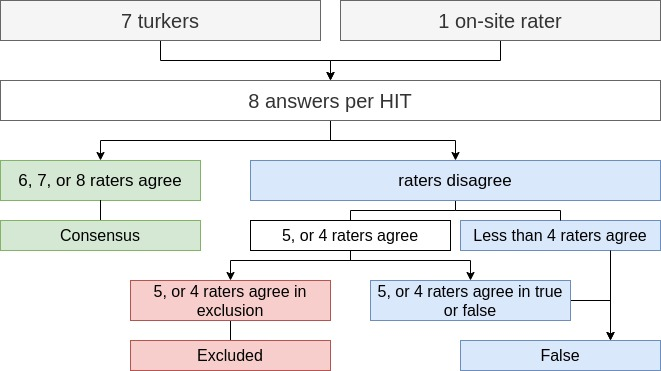
\includegraphics[width=0.8\linewidth]{images/chapter_6/figure_3.jpg}
\caption[Flowchart Illustrating How to Reach Majority Consensus]{Flowchart illustrating how to reach majority consensus, according to the answers provided by the workers plus our extra rater on site.} \label{fig3}
\end{figure}

To further assess the quality and challenges of curating the PGR dataset and validate the previous approach, a domain expert with a Bioinformatics background and experience in using and curating corpora also curated the relations in Task 2. 

\paragraph{Deep Learning Systems}

To further access the quality of the crowdsourced curated dataset, we applied it to two distinct deep learning systems that target the biomedical domain: BiOnt \citep{sousa2020biont} and BioBERT \citep{lee2020biobert}. For comparison, we tested both the original PGR dataset and the crowdsourced Amazon dataset, as well as combinations between the two (detailed in Table \ref{tab5}).

The BiOnt system is a deep learning system based on the BO-LSTM system \citep{lamurias2019bo} that is used to extract and classify relations via long short-term memory networks and biomedical ontologies. This system detects and classifies ten types of biomedical relations, such as human phenotype-gene relations. It takes advantage of domain-specific ontologies, like the Human Phenotype Ontology (HPO) \citep{kohler2017human} and the Gene Ontology (GO) \citep{ashburner2000gene}. The BiOnt system represents each entity as the sequence of its ancestors in their respective ontology.

The BioBERT system is a pre-trained biomedical language representation model for biomedical text mining based on the BERT \citep{devlin2019bert} architecture. This system can perform diverse biomedical text mining tasks, namely NER, RE, and Question Answering (QA), when trained on large-scale biomedical corpora. The novelty of the architecture is that their authors designed these systems (BioBERT and BERT) to pre-train deep bidirectional representations by joint conditioning on both the left and right context in all layers. This feature allows easy adaptation to several tasks without loss in performance.

\section{Results and Discussion}

\subsection{Ratings Statistics}

To assess the performance of the workers, we conducted some statistical analyses, including the time spent on average rating each sentence. Figure \ref{fig4} and \ref{fig5} reflect the average time spent by the workers with each sentence, with a cutoff of 50 seconds (using box plot and standard deviation analysis). We decided to set the cutoff for work time to 50 seconds because we considered that was enough time for a worker to make an assessment, and anything longer than that was probably the worker having a mid-task break (the longest time for a HIT completion was 40322 seconds, about 11 hours). 

\begin{figure}[H]
\centering
\begin{minipage}{0.48\textwidth}
\centering
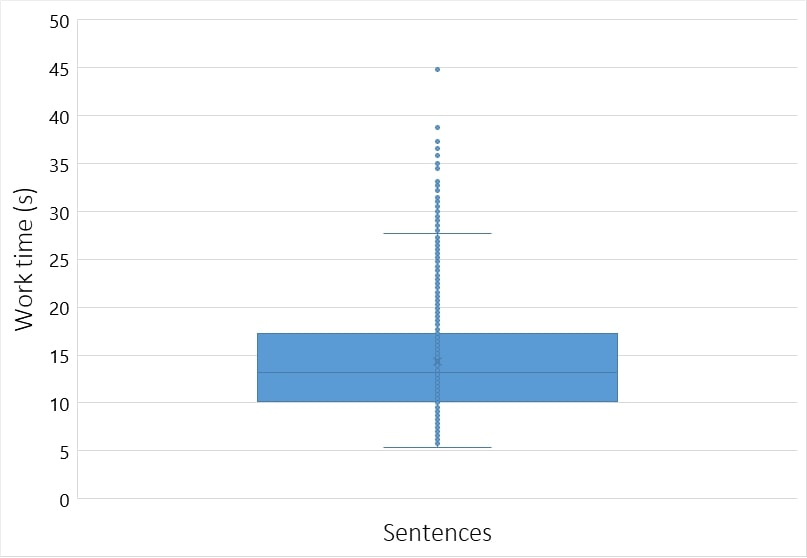
\includegraphics[width=0.97\linewidth]{images/chapter_6/figure_4.jpg}
\caption[Box Plot Expressing the Average Worker Work Time Distribution]{Box plot expressing the average worker work time distribution (in seconds) per sentence (with a cutoff of 50 seconds).}\label{fig4}
\end{minipage}
\hfill
\begin{minipage}{0.48\textwidth}
\centering
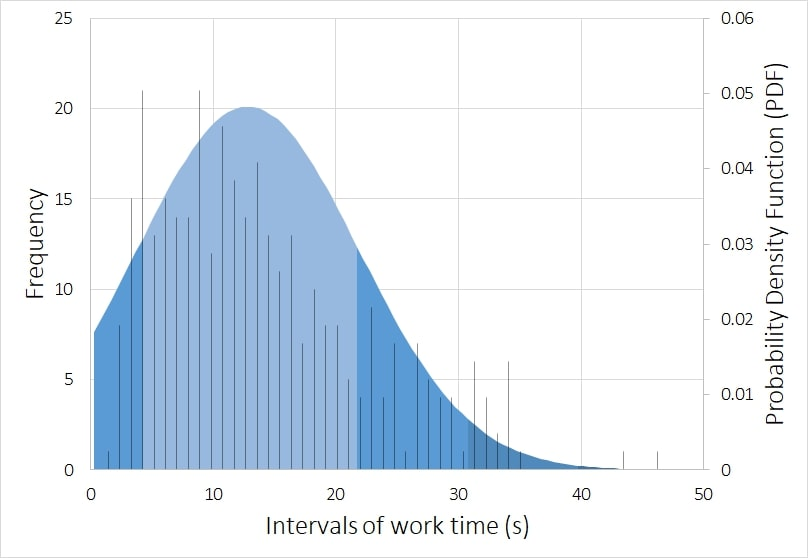
\includegraphics[width=0.97\linewidth]{images/chapter_6/figure_5.jpg}
\caption[Standard Deviation Expressing the Average Worker Work Time Distribution]{Standard deviation expressing the average worker work time distribution (in seconds), and the histogram of the occurrence events (with a cutoff of 50 seconds).}\label{fig5}
\end{minipage}
\end{figure}

Our domain expert did a similar time self-evaluation, which resulted in an average of about 20 seconds per sentence (for Task 2). The domain expert consulted some abstracts to clarify whether an abbreviation refers to a gene or other type of entity for a specific sentence. Through Figures \ref{fig4} and \ref{fig5}, it is possible to assess that workers took an average of 13 seconds per HIT (sentence). By comparing this time to the average time taken by our domain expert (20 seconds), it is possible to question the level of attention with which our workers performed their ratings, questioning the trust that we can deposit in MTurk crowdsourcing. However, taking into consideration that our domain expert took some time checking some abstracts to which workers did not have access, it can justify the differences in average time.

To further characterize the workers that performed our tasks, we checked their WorkerId tab in the results file provided by MTurk. There, we realized that six sentences were rated but did not have an associated WorkerId and that both tasks (7983 relations, 22255 HITs) were performed by only 64 different workers, making, on average, 348 HITs per worker. Therefore, if we had a malicious worker that classified their respective HITs randomly, it would damage the whole dataset. The MTurk platform should guarantee a more diverse group of workers working on the same task since that is what employees expect, even to avoid some biased ratings or a more strict selection process.

\subsection{Inter-rater Agreement}

Table \ref{tab3} presents the inter-rater agreement score, using both Fleiss’ kappa \citep{mchugh2012interrater} and Krippendorff’s alpha \citep{krippendorff2011computing} metrics, for the dataset corresponding to Task 2, considering only the Amazon workers, the Amazon workers plus the extra rater (on-site), and the extra rater (on-site) plus the domain expert.

\begin{table}[h]
\centering
\caption[Inter-rater Agreement Scores]{The inter-rater agreement score, using both Fleiss’ kappa and  Krippendorff’s alpha metrics, considering only the Amazon workers, the Amazon workers plus the extra rater (on-site), and the extra rater (on-site) plus the domain expert (Task 2). AW stands for Amazon Workers}\label{tab3}
\begin{tabular}{lccc}
\hline
\multirow{2}{*}{Inter-rater agreement metric} & \multicolumn{3}{c}{Inter-rater agreement} \\
\cline{2-4}
& AW & AW + extra rater (on-site) & Extra rater (on-site) + expert \\
\hline
Fleiss' kappa & 0.2028 & 0.2050 & 0.6549 \\
Krippendorff’s alpha & 0.2029 & 0.2051 & 0.6550 \\
\hline
\end{tabular}
\end{table}

Given the small number of workers working on Task 2 (33) and the high number of sentences to rate (2389), it is challenging to find an inter-rater agreement metric that can return an accurate agreement value between the workers. Fleiss’ kappa metric assumes that the raters are deliberately chosen and fixed, while Krippendorff’s alpha metric is indicated when we have multiple raters and multiple possible ratings. Since none of the two cases is precisely right, we do not have a metric that fully expresses the results of our experiment with Task 2. We can say that probably the agreement between raters was only moderate (on a qualitative scale). Some of the reasons for moderate agreement could be difficulties in understanding the task, complex biomedical sentences that are beyond the scope of the average worker, or random answers provided by malicious workers. 

It was particularly interesting to have an extra rater (on-site) that could express doubts while performing the task. Some of these doubts could be the ones that the workers had, while others we considered to be beyond their expertise. For our on-site rater, one of the most prominent problems was if the gene entities tagged were, in fact, gene entities or their proteins products that frequently share the same names. One could argue that a relation between a gene product and a human phenotype implies a relation between a gene and a human phenotype. Nonetheless, the extra rater considered that these relations hold even if the mention was of a protein and not the gene if this distinction was not clear by the sentence (only when reading the abstract or full-text article) or if the gene name was not capitalized. This particular problem was not one that a person not familiar with Biochemistry related domains would have. However, assessing if an abbreviation that is used both as a gene name and in other biomedical topics (e.g., disease abbreviation) is a gene is a transversal problem for both the workers and our extra rater on-site. 

The difficulties that our extra-rater experienced are evident in the inter-rater agreement between this rater and our domain expert. One example sentence where they disagreed was:

\textit{While examining pedigrees of JEB patients with \textbf{LAMA3} mutations, we observed that heterozygous carriers of functional null mutations displayed subtle enamel pitting in the absence of \textbf{skin fragility} or other JEB symptoms.} (PMID:27827380)

where the domain expert considered a true relation and the extra-rater a false relation, this happens because the relation is one of negation (absence) which often confuses non-experts with being false. However, an implication of relation of any sort is a true relation which can then be classified as positive or negative. This confusion is also noticeable by the diversity in the workers' answers for this sentence (four classified as true, two as false, and one as an error).
 
\subsection{Corpus Statistics}


Table \ref{tab4} presents the final numbers both in total count and percentage for each task. For Task 2, we considered the majority consensus described previously and the domain expert numbers separately.

\begin{table}[h]
\centering
\caption[Final Relations Counts]{The original and final numbers both in total count and percentage, for Tasks 1 and 2, of true, false, excluded and total relations, considering the majority consensus and the domain expert numbers separately. AW stands for Amazon Workers}\label{tab4}
\newcolumntype{A}{ >{\centering\arraybackslash} m{2cm} }
\begin{tabular}{lAcccc}
\hline
\multirow{2}{*}{Dataset} & & \multicolumn{4}{c}{Relations} \\
\cline{3-6}
\multicolumn{2}{c}{} & True & False & Excluded & Total\\
\hline
Task 1 (70\%) & Original & 1751 (31.41\%) & 3823 (68.59\%) & - & 5574 (100\%)\\
& AW & 4220 (75.71\%) & 283 (5.08\%) & 1071 (19.21\%) & 4503 (80.79\%)\\
\hline
Task 2 (30\%) & Original & 729 (30.51\%) & 1660 (69.49\%) & - & 2389 (100\%)\\
& AW + extra rater (on-site) (after reaching consensus) & 41179 (49.35\%) &613 (25.66\%) & 240 (10.05\%) & 1792 (75.01\%)\\
& Expert & 1281 (53.62\%) & 343 (14.36\%) & 765 (32.02\%) & 1624 (67.98\%)\\
\hline
\end{tabular}
\end{table}

From analyzing Table \ref{tab4}, what becomes immediately evident is the inversion between the number of true and false relations from the original datasets to the Amazon crowdsourced datasets. These final numbers demonstrate quite clearly that most relations described in the original PGR dataset as false were, in fact, true. This inversion can be due to how the PGR dataset was built, using a gold standard knowledge base of human phenotype-gene relations. This knowledge base, at the time of the dataset creation, was quite incomplete since, for instance, if a child's ontological term had a relation with a gene, its immediate parent would not necessarily share the same relation, which should be explicit. Thus, these parent concepts in PGR relations would always hold false. 

Also, understanding the difference between an annotation error and a false relation requires more expertise than the one that MTurk provides and that inexperienced raters have (even if in the field). Thus, to differentiate between false relations and an annotation error, we need expert knowledge, such as in the following annotation error example:

\textit{We show that the \textbf{miR}-106b-25 cluster upregulates NOTCH1 in multiple breast \textbf{cancer} cell lines, representing both estrogen receptor (ER+) and triple negative breast cancer (TNBC) through direct repression of the E3 ubiquitin ligase, NEDD4L.} (PMID:29662198)

where the workers had difficulties accessing that miR just by itself is not a gene entity but stands for microRNA genes (a large group of genes).

\subsection{Deep Learning Impact}

Table \ref{tab5} presents the performance of both the original PGR dataset and the crowdsourced Amazon dataset, and combinations between the two, on the BiOnt \citep{sousa2020biont} and BioBERT (version 1.1) \citep{lee2020biobert} systems, in terms of precision, recall, F-measure, and accuracy. To assess the performance of the dataset (before and after crowdsourcing) when applied to deep learning systems, we used the suggested parameters by the authors of each system. The only exception to the default parameters, since we had a class imbalance, was to add a class weight of 5 to the label false to both systems (the full multiplier to balance was approximately 14.9 for the Task 1 dataset). The full multiplier is a result of dividing the percentage of true relations by the percentage of false relations for the training dataset. For the class weight, we chose a number between 1 and the full multiplier, which is usually the standard practice \citep{chen2018efficient}, to maintain a more accurate representation of the natural unbalance between labels when applying the models to real-world data. Using this class weight translates to treating every training instance with the label false as five instances of the label true, meaning that in the loss function, we assign a higher value to these instances. Hence, the loss becomes a weighted average, where the weight of each sample is specified by the class weight and its corresponding class, providing a weight or bias for each output class. To achieve this, we had to alter the loss function of the BioBERT system to allow class weights.

\begin{table}[h]
\centering
\caption[Performance Metrics of BiOnt and BioBERT with the PGR Dataset]{Precision, recall, F-measure, and accuracy of the application of the PGR dataset (original, new, and combinations between the two) to the BiOnt and BioBERT systems. The highest scores for each metric are presented in bold}\label{tab5}
\newcolumntype{B}{ >{\raggedright} m{5cm} }
\begin{tabular}{lBcccc}
\hline
Method & & Precision & Recall & F-measure & Accuracy \\
\hline
BiOnt & PGR & 0.8140 & 0.3070 & 0.4459 & 0.4821\\
& Amazon (train) + PGR (test) & 0.7000 & 0.9825 & 0.8175 & 0.7024\\
& Amazon (train) + Amazon workers consensus (test) & 0.6810 & 0.9670 & 0.7992 & 0.6726\\
& Amazon (train) + Expert (test) & \textbf{0.8142} & 0.9721 & \textbf{0.8861} & \textbf{0.7989}\\
& Amazon workers consensus (train) + PGR (test) & 0.6880 & 0.8509 & 0.7608 & 0.6369\\
& Expert (train) + PGR (test) & 0.6894 & \textbf{0.9737} & 0.8072 & 0.6845\\
\hline
BioBERT & PGR & \textbf{0.8542} & 0.3445 & 0.4910 & 0.5143\\
& Amazon (train) + PGR (test) & 0.6744 & 0.9856 & 0.8000 & 0.6775\\
& Amazon (train) + Amazon workers consensus (test) & 0.6700 & 0.9763 & 0.7946 & 0.6680\\
& Amazon (train) + Expert (test) & 0.8103 & \textbf{0.9906} & \textbf{0.8915} & \textbf{0.8096}\\
& Amazon workers consensus (train) + PGR (test) & 0.7315 & 0.9160 & 0.8134 & 0.7143\\
& Expert (train) + PGR (test) & 0.7857 & 0.8319 & 0.8082 & 0.7314\\
\hline
\end{tabular}
\end{table}

The deep learning systems performance is quite similar, with BioBERT achieving slightly better results. In both systems, the performance of the new PGR dataset (through MTurk crowdsourcing) was superior to that of the original PGR dataset, with a slight decrease in precision but a considerable gain in the recall. We included the accuracy metric to consider the ability to recognize true negatives as well (due to the class imbalance). The best performance overall was the Amazon MTurk (Task 1) as the training corpus and the expert (Task 2) as the test corpus. This performance can be due to the amount of available training data in Task 1 and the more reliable test set from the domain expert. The PGR original test set underperformed probably due to its small size, which was not being representative of the data (260 relations).  Also, other experiences with using the majority consensus (Task 2) and the expert (Task 2) as training sets showed that these smaller corpora also hold the ability to train a model. 

\section{Conclusion and Future Directions}

This work describes our proposal for a complete pipeline for RE crowdsourcing. The pipeline  generated an openly available new release of the PGR dataset, as well as a domain expert revision into 30\% of the original dataset. Additionally, we assessed MTurk workers' performance by comparing them to an extra rater on-site and to a domain expert.   Moreover, we applied the new dataset as training data in two state-of-the-art deep learning systems (BiOnt \citep{sousa2020biont} and BioBERT \citep{lee2020biobert}) to measure the usefulness of the annotations. This study showed that it is possible to use the wisdom of the crowd to at least improve existing silver standard datasets since, in our case, it was able to exclude previous annotation errors (16.46\%) and modify wrongly labelled relations. This improvement had a significant impact on model training since we had a 0.3494 average increase in F-measure, taking into account all the experiences when comparing it with the original PGR dataset. 

Regarding future work, it will be interesting to improve on the existing pipeline by providing different guidelines and assessing if that would make a difference in performance. Also, we can differentiate between what constitutes a false and a negative relation. To solve the lack of domain expertise of MTurk workers, we could create a specialized crowdsourcing platform for the RE biomedical field, similar to the one developed by the company Unbabel that focuses on translation \citep{gracca2018unbabel}, as well as other biomedical crowdsourcing projects \citep{tsueng2020applying,kleffner2017foldit}. Finally, we could apply the same methods to datasets from other biomedical domains and assess the differences in performance. 

\clearpage
\section{Supplementary Material}


\begin{figure}[h]
\centering
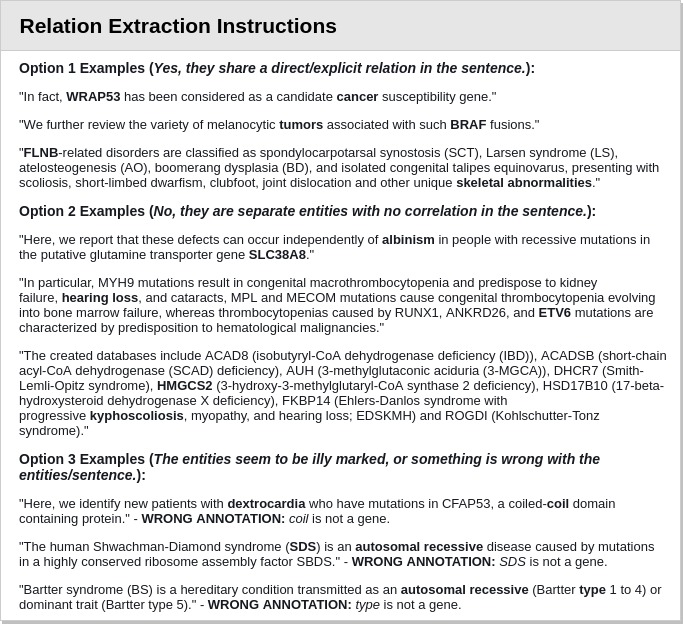
\includegraphics[width=0.8\linewidth]{images/chapter_6/supplementary_material_figure_1.jpg}
\caption[Amazon MTurk Guidelines]{The guidelines, in the form of examples of answers to different annotations, that were presented to the workers.} \label{sfig1}
\end{figure}



\hypertarget{7}{}

\rhead{Real-Word Assessments}
\lhead{Chapter 7}

\chapter[Real-Word Assessments]
{\huge Real-Word Assessments} % \\
% \Large \textmd{Diana Sousa, Andre Lamurias, and Francisco M. Couto}}

\vspace{-1.6cm}

% Gray Line
\begingroup
\color{black}
\par\noindent\rule{\textwidth}{0.4pt}
\endgroup

\noindent{This chapter compiles all other research work conducted throughout this thesis by dividing each contribution into a section summarising its motivation and the work developed. This work includes solo and group participation in workshops, challenges, a doctoral consortium, and other adjacent journal contributions, all corresponding to real-world assessments of the systems and approaches developed in this thesis.} 

\section{Improving Accessibility and Distinction Between Negative Results in Biomedical Relation Extraction}

Every year, researchers organise the Biomedical Linked Annotation Hackathon (BLAH) series to promote interoperability among text mining resources and their efficient use or reuse, particularly in the mix with others. In 2020, BLAH6 addressed issues regarding biomedical literature and social media mining \citep{kim2020editor}. 

This thesis participation in BLAH6 targeted the improvement of accessibility and distinction between negative results in biomedical Relation Extraction (RE). Accessible negative results are relevant for researchers and clinicians to limit their search space and prevent the costly re-exploration of research hypotheses. However, most biomedical RE datasets do not seek to distinguish between a false and a negative relation between two biomedical entities. Furthermore, datasets created using distant supervision techniques also have false negative relations constituting undocumented/unknown relations (missing from a knowledge base). We proposed to improve the distinction between these concepts by revising a subset of the relations marked as false on the phenotype-gene relations corpus and giving the first steps to automatically distinguish between the false (F), negative (N), and unknown (U) results. The work resulted in a sample of 127 manually annotated FNU relations and a weighted F-measure of 0.5609 for their automatic distinction. The full application note is available at \hyperlink{AC}{Appendix C}:

\begin{itemize}[label=]
  \item \textbf{Sousa, D.}, Lamurias, A., and Couto, F. M. (2020). \textbf{Improving Accessibility and Distinction Between Negative Results in Biomedical Relation Extraction}. Genomics \& Informatics, 18(2):1-4. \citep{sousa2020improving} \footnote{\url{https://github.com/lasigeBioTM/blah6}}
\end{itemize}


\section{Generating Biomedical Question Answering Corpora From Q\&A Forums}

As presented in Chapter 2, Question Answering (QA) is a natural language processing task that aims at obtaining relevant answers to user questions. In 2020, while some progress had been made in this area, biomedical questions were still a challenge to most QA approaches due to the complexity of the domain and the limited availability of training sets. 

Thus, we presented a method to automatically extract question-article pairs from Q\&A web forums, which could be used for document retrieval, a crucial step of most QA systems. The proposed framework extracts from selected forums the questions and the respective answers that contain citations. This way, QA systems based on document retrieval can be developed and evaluated using the question-article pairs annotated by users of these forums. We generated the BiQA corpus by applying our framework to three forums, obtaining 7,453 questions and 14,239 question-article pairs. We evaluated how the number of articles associated with each question and the number of votes on each answer affect the performance of baseline document retrieval approaches. Also, we demonstrated that the articles given as answers are significantly similar to the questions and trained a state-of-the-art deep learning model that performed similarly to using a dataset manually annotated by experts. The proposed framework can be used to update the BiQA corpus from the same forums as new posts are made and from other forums that support their answers with documents. The full journal article is available at \hyperlink{AD}{Appendix D}:

\begin{itemize}[label=]
    \item{Lamurias, A., \textbf{Sousa, D.}, and Couto, F. M. (2020). \textbf{Generating Biomedical Question Answering Corpora From Q\&A Forums}. IEEE Access, 8:161042–161051. (Q1 Scimago) \citep{lamurias2020generating}} \footnote{\url{https://github.com/lasigeBioTM/BiQA}}
\end{itemize}

\section{COVID-19: A Semantic-Based Pipeline for Recommending Biomedical Entities}

During the research work developed in this thesis, an unprecedented global pandemic emerged due to the widespread coronavirus SARS-CoV-2. This pandemic had a dramatic impact worldwide, leading scientists in all different domains to step up to positively influence the outbreak's outcome.   

Accordingly, the \ac{ACL} community in April 2020 decided to take action. Given the vast quantities of unstructured text being written at the time, relevant information was becoming increasingly hard to uncover. Hundreds of articles were written daily on coronavirus, and the general public interest and response resulted in millions of social media posts. Both were valuable sources of information to understand and support the best clinical management of the disease. Automating the organization and identification of this information was critical \citep{nlp-covid19-2020-nlp}. Thus, researchers decided to create the 1\textsuperscript{st} Workshop on Natural Language Processing (NLP) for COVID-19, an ever-encompassing workshop, with many submissions supported by resources such as the CORD-19 dataset created by the Allen Institute for \acl{AI} \citep{wang-etal-2020-cord}, a resource of scientific papers on COVID-19 and related historical coronavirus research.

Our submission had the goal of recommending biomedical entities to scientific researchers  \citep{barros2020covid}. For instance, to recommend new chemical compounds to researchers with similar interests to peers working on those compounds. To this end, we used the CORD-19 dataset, performed Named-Entity Recognition (NER) to identify/extract biomedical entities, then RE to further our knowledge about the interconnections of those entities, and finally, Recommendation taking into account research articles authors' and their biomedical entities of interest. Results showed a precision@k of 80\%, demonstrating this pipeline's potential to uncover information on the vast amounts of data created up until then. The full workshop article is available at \hyperlink{AE}{Appendix E}:

\begin{itemize}[label=]
    \item{Barros, M., Lamurias, A., \textbf{Sousa, D.}, Ruas, P., and Couto, F. M. (2020). \textbf{COVID-19: A Semantic-Based Pipeline for Recommending Biomedical Entities}. In Proceedings of the 1\textsuperscript{st} Workshop on NLP for COVID-19 (Part 2) at EMNLP 2020, pages 1–9, Online. Association for Computational Linguistics. (Core A) \citep{barros2020covid}} \footnote{\url{https://github.com/lasigeBioTM/knowledge-extraction-from-CORD-19}}
\end{itemize}

\section{lasigeBioTM at BioCreative VII Track 1: Text Mining Drug and Chemical - Protein Interactions using Biomedical Ontologies}

Community challenges are often organized, targeting biomedical NLP and text mining.
BioCreative was first organized in 2004, and it consisted of identifying gene mentions and Gene Ontology (GO) terms in articles and gene name normalization \citep{hirschman2005overview}. Since then, seven more editions of this challenge have been organized with various tasks. In 2021, the BioCreative VII Track 1 aimed to promote the development and evaluation of systems that can automatically detect relations between chemical compounds/drugs and genes/proteins.

Identifying biomedical relations is necessary to advance our understanding of biological processes and is particularly relevant for applications in precision medicine. In the BioCreative VII Track 1, our team, lasigeBioTM, had as its primary goal the extraction and classification of drug and chemical-protein interactions. Our team adapted an existing neural network system, BiOnt, incorporating external knowledge from biomedical ontologies. To perform Track 1, we used the GO and the Chemical Entities of Biological Interest (ChEBI) ontology. We submitted different runs considering the use of features such as class weights and post-processing rules. However, due to time constraints, we could only make some of the initial planned improvements, and our results were below the mean performance of the participating teams. Still, we took the first steps towards this adaption, and we can now continue improving this system to reach state-of-the-art performance. Nonetheless, this work was chosen for presentation due to the approach's originality. The full challenge article is available at \hyperlink{AF}{Appendix F}:

\begin{itemize}[label=]
    \item{\textbf{Sousa, D.}, Cassanheira, R., and Couto, F. M. (2021). \textbf{lasigeBioTM at BioCreative VII Track 1: Text Mining Drug and Chemical-Protein Interactions Using Biomedical Ontologies}. In Proceedings of the BioCreative VII Challenge Evaluation Workshop, pages 1–4, Online. Association for Computational Linguistics. \citep{sousalasigebiotm}} \footnote{\url{https://github.com/lasigeBioTM/biocreativeVII}}
\end{itemize}

\section{Deep Learning System for Biomedical Relation Extraction Combining External Sources of Knowledge}

Doctoral Consortiums are events where PhD students are expected to present their ongoing and future research. In 2021, the European Conference on Informational Retrieval (ECIR) made a call for Doctoral Consortium papers targeting second-year PhD students where accepted students would have the opportunity to be matched with a specialized mentor to advance their research work further. The proposal for the doctoral work detailed in this thesis was presented and discussed. The full Doctoral Consortium paper is available at \hyperlink{AG}{Appendix G}:

\begin{itemize}[label=]
    \item{\textbf{Sousa, D.} (2021). \textbf{Deep Learning System for Biomedical Relation Extraction Combining External Sources of Knowledge}. In Advances in Information Retrieval: 43\textsuperscript{rd} European Conference on IR Research, pages 688–693, Berlin, Heidelberg. Springer. (Core A) \citep{sousa2021deep}}
\end{itemize}

\section{COVID-19 Recommender System Based on an Annotated Multilingual Corpus}

In 2021, we once again participated in the BLAH series. The BLAH7 edition aimed at finding NLP-based solutions to tackle the COVID-19 pandemic \citep{kim2021editor}.

Tracking the most recent advances in Coronavirus disease 2019 (COVID-19)-related research was essential, given the disease's novelty and its impact on society. However, with the publication pace speeding up, researchers and clinicians required automatic approaches to keep up with the incoming information regarding the disease. A solution to this problem required the development of text mining pipelines, the efficiency of which strongly depends on the availability of curated corpora. However, there was a lack of COVID-19-related corpora, even more if considering other languages besides English. This project's main contribution was the annotation of a multilingual parallel corpus and the generation of a recommendation dataset (EN-PT and EN-ES) regarding relevant entities, their relations, and recommendation, providing this resource to the community to improve the text mining research on COVID-19-related literature. The full journal article is available at \hyperlink{AH}{Appendix H}:

\begin{itemize}[label=]
    \item{Barros, M.\footnote[*]{Authors contributed equally to this research}, Ruas, P.\textsuperscript{*}, \textbf{Sousa, D.}\textsuperscript{*}, Bangash, A. H., and Couto, F. M. (2021). \textbf{COVID-19 Recommender System Based on an Annotated Multilingual Corpus}. Genomics \& Informatics, 19(3):1-7. \citep{barros2021covid}} \footnote{\url{https://github.com/lasigeBioTM/blah7}}
\end{itemize} 

\section{lasigeBioTM at SemEval-2023 Task 7: Improving Natural Language Inference Baseline Systems with Domain Ontologies}

One community challenge that often targets the biomedical domain is SemEval. SemEval-2023 Task 7 – Multi-Evidence Natural Language Inference for Clinical Trial Data (NLI4CT) was based on the NLI4CT dataset, which contains two tasks on breast cancer Clinical Trials Reports (CTRs) \citep{jullien-2023-nli4ct}. Firstly, to determine the inference relation between a natural language statement and a CTR. Secondly, to retrieve supporting facts from the CTR(s) to justify the predicted relation.

CTRs contain highly valuable health information from which Natural Language Inference (NLI) techniques determine if a given hypothesis can be inferred from a given premise. CTRs are abundant with domain terminology with particular terms that are difficult to understand without prior knowledge. Thus, we proposed to use domain ontologies as a source of external knowledge that could help
with the inference process in the SemEval-2023  Task 7 (NLI4CT). Our approach targeting subtask 1: Textual Entailment, resorted to Ontologies, NLP techniques, such as tokenization and named-entity recognition, and rule-based approaches. We could show that inputting annotations from domain ontologies improved the baseline systems. The full challenge article is available at \hyperlink{AI}{Appendix I}:

\begin{itemize}[label=]
    \item{Conceição S. I. R., \textbf{Sousa, D. F.}, Silvestre, P. M., and Couto, F. M. (2023). \textbf{lasigeBioTM at SemEval-2023 Task 7: Improving Natural Language Inference Baseline Systems with Domain Ontologies}. (Accepted)} \footnote{\url{https://github.com/lasigeBioTM/SemEval2023_Task-7}}
\end{itemize}

\section{LASIGE and UNICAGE Solution to the NASA LitCoin NLP Competition}

The 2022 LitCoin NLP Challenge was a part of the NASA Tournament Lab, hosted by the National Center for Advancing Translational Sciences (NCATS) and the National Library of Medicine (NLM). The competition aimed to create a data-driven technological solution that leverages the vast volumes of biomedical publications published daily to advance the biomedical field by increasing discoverability and formulating new research hypotheses. Specifically, the goal was to extract scientific concepts from scientific articles (Part 1), connect them by generating knowledge assertions, and label them as novel findings or background information (Part 2). 

Biomedical NLP tends to become cumbersome for most researchers, frequently due to the amount and heterogeneity of text to be processed. To address this challenge, the industry is continuously developing highly efficient tools and creating more flexible engineering solutions. Our work presented the integration between industry data engineering solutions for efficient data processing and academic systems developed for Named Entity Recognition (LasigeUnicage\_NER) and Relation Extraction (BiOnt). Our design reflects an integration of those components with external knowledge in the form of additional training data from other datasets and biomedical ontologies. We used this pipeline in the 2022 LitCoin NLP Challenge, where our team LasigeUnicage was awarded the 7\textsuperscript{th} Prize out of approximately 200 participating teams, reflecting a successful collaboration between the academia (LASIGE) and the industry (Unicage). The full article is available at \hyperlink{AJ}{Appendix J}:

\begin{itemize}[label=]
    \item{Ruas, P.\footnote[†]{Authors contributed equally to this research}, \textbf{Sousa, D. F.}\textsuperscript{†}, Neves, A.\textsuperscript{†}, Cruz, C., and Couto, F. M. (2023). \textbf{LASIGE and UNICAGE Solution to the NASA LitCoin NLP Competition}. (Submitted)} \footnote{\url{https://github.com/lasigeBioTM/Litcoin-Lasige_Unicage}}
\end{itemize}




\hypertarget{8}{}

\rhead{General Discussion and Conclusions}
\lhead{Chapter 8}

\chapter[General Discussion and Conclusions]
{\huge General Discussion and Conclusions}

\vspace{-1.6cm}

% Gray Line
\begingroup
\color{black}
\par\noindent\rule{\textwidth}{0.4pt}
\endgroup

\noindent{In the foreseeable future, the amount of written literature available online in an unstructured or semi-structured way will continue to grow. With this growth in the number of written resources, the necessity for developing automated methods to process it becomes increasingly more relevant. Lately, even the non-scientific community has become aware of the problem and possibilities through the emergence of accessible generative models (i.e., GPT derivatives). However, even with the advances made until the writing of this thesis on automated data retrieval and generation, the problem of biomedical Relation Extraction (RE) still needs to be addressed on several fronts, given the lack of liability, expertise, and explainability of these approaches.}

Biomedical data is complex and has yet to be fully understood or captured by traditional Large Language Models (LLM). We can find biomedical relations in various scientific sources and several languages. However, the amount of written resources prevents researchers and clinicians from knowing or inferring all possible associations and dissociations, leading to experimental repetition. 

In this manuscript, the main body of work tackles the integration of external knowledge into biomedical RE systems, making them predecessors of what we more recently defined as multimodal systems that integrate more than one data format/source. Beyond integrating knowledge, this thesis explores new ways of creating biomedical RE datasets and, through workshops and challenges, different biomedical applications of the principals reported in the main body of work. The following sections summarise the main thesis contributions and future work in biomedical RE. 

\section{Summary of Contributions}

This section provides an overview of the contributions regarding each of the objectives defined in the introductory chapter: Deep Learning with External Knowledge and Evaluation.

This thesis first presents three deep learning systems with external knowledge injection (Objective 1). These are BiOnt (Chapter 3), K-BiOnt (Chapter 4), and K-RET (Chapter 5).

BiOnt is a BiLSTM-based system with two annotation layers that learn different information about the entities in candidate relations. The system annotations layers' are employed using four types of biomedical ontologies, namely, the \acl{GO} (GO), the \acl{HPO} (HPO), the \acl{DO} (DO), and the \acl{ChEBI} (ChEBI), regarding gene products, phenotypes, diseases, and chemical compounds, respectively. The two annotation layers represent the concatenation of ontological ancestors of the entities in the candidate relation and the common ancestors between those entities when considering relations between the same type of entities. BiOnt surpassed the previous state-of-the-art in the three datasets used for evaluation. 

Following BiOnt, to test other possibilities of knowledge injection and benefit of the ideas of other fields, K-BiOnt employed the principals of \acl{KG} (KG)-based recommendation. K-BiOnt used multiple biomedical \ac{KG} to add features to the entities in a candidate relation. The deep learning system combined BiOnt and a \ac{KG}-based recommendation system. The concepts of item and user were used to describe the entities in a candidate relation and Ontological KGs to add information (i.e., features) to each item, meaning only entities covered by KGs entries had features. Results showed that allying the two approaches can help detect more rare/underexpressed relations. 

Finally, given the widespread use of BERT, K-RET was developed using BERT as a pre-training model and fine-tuned to include knowledge directly in the training data text. K-RET allows injecting knowledge only to the entities in the candidate relation, to additional contextual entities of interest, using multiple knowledge sources, and to multi-token entities. K-RET significantly outperformed baseline BERT systems' performance, particularly in detecting drug-drug interactions. 

This thesis demonstrated that one could use state-of-the-art deep learning techniques with added external knowledge as complementary data to create effective and reproducible biomedical RE systems that beat the previous state-of-the-art performance when validated on gold standard datasets, accomplishing the first objective. 

After the three systems summarized above, in Chapter 6, this work presents an approach to creating new biomedical RE datasets (Objective 2). 

The approach explores the application of distant supervision techniques to retrieve candidate relations from unstructured text and their validation through different techniques, such as a crowdsourcing platform with pre-defined settings. Results demonstrated the benefit of having even non-experts revise a human phenotype-gene relations dataset using state-of-the-art systems for comparison. 

This work successfully created a pipeline to construct more reliable and less expensive RE datasets by employing distant supervision allied with crowdsourcing, validating the second objective. 

Other explorations of biomedical data and real-world assessments of the approaches and systems developed in this work are reported in Chapter 7 and include considering negative relations, their accessibility and distinction, using biomedical \acl{NLP} (NLP) techniques to create a \acl{QA} (QA) dataset from Q\&A forums on biomedical sciences, and using COVID-19-related literature recommendations in a multilingual environment. 

\section{Future Work}

While recent advances in biomedical RE are exciting and open new opportunities for data exploration and comprehension, the emergence of deep learning methods catapulted the necessity for explainability. The lack of explainability of deep learning models makes it hard to trust predictions, specifically when these target the highly complex biomedical domain. The injection of knowledge into deep learning systems can contribute to more explainable predictions as presented throughout this thesis. However, we can still not fully follow the path from input to prediction when dealing with deep learning. The path forward passes by not only explaining or justifying predictions but also defining what degree of explainability is adequate and necessary for each end-user.

Further, ethical Artificial Intelligence (AI) is a field that aims that AI systems go towards greater ecological integrity and social justice. A study by \cite{strubell2019energy} illustrated that training a single deep learning NLP model can lead to approximately 600,000 lb of carbon
dioxide emissions, which can be addressed by the development of minimal resources models. Reproducibility is also an ongoing issue in the field, given that there are systems whose code is not shared. Frequently, authors justify this choice through privacy claims. However, there should always be a way to at least partially replicate the system that could be guaranteed by the venues that accept those types of publications. All community members continued sharing and discussing of open-sourced systems contribute to significant advances in the field. These and other concerns, such as biased datasets and taking into account $n$-ary relations (i.e., more than two entities), should be addressed and made a priority by the groups working on biomedical text mining.

\pagestyle{plain}  % no more header 

\newpage
\renewcommand\bibname{References}
\bibliography{references}
\bibliographystyle{apalike}



\chaptertitlefont{\LARGE}



\hypertarget{a}{\appendix}
\hypertarget{AA}{\chapter{Using Neural Networks for Relation Extraction from Biomedical Literature}}
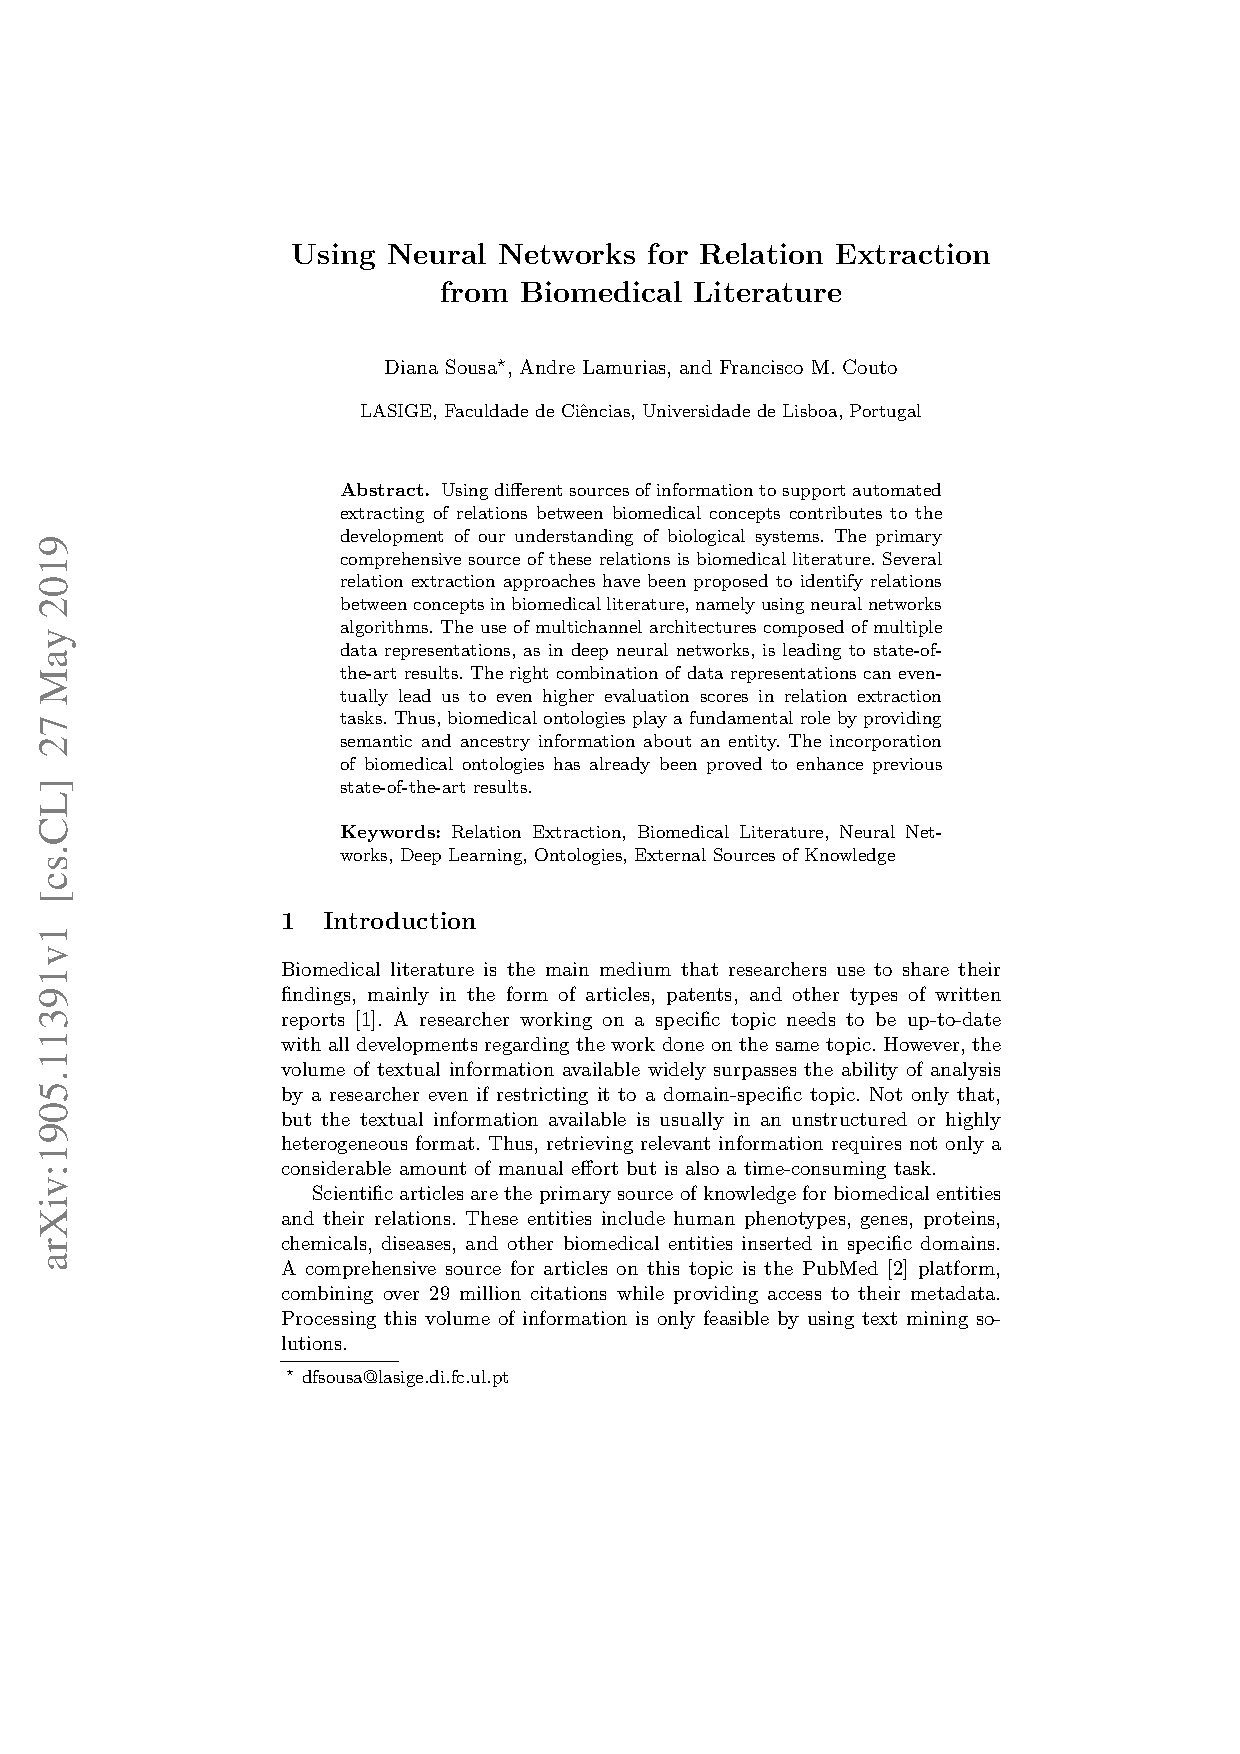
\includepdf[pages=-,scale=1]{articles/1905.11391.pdf}

\hypertarget{AB}{\chapter{BiOnt: Deep Learning using Multiple Biomedical Ontologies for Relation Extraction}}
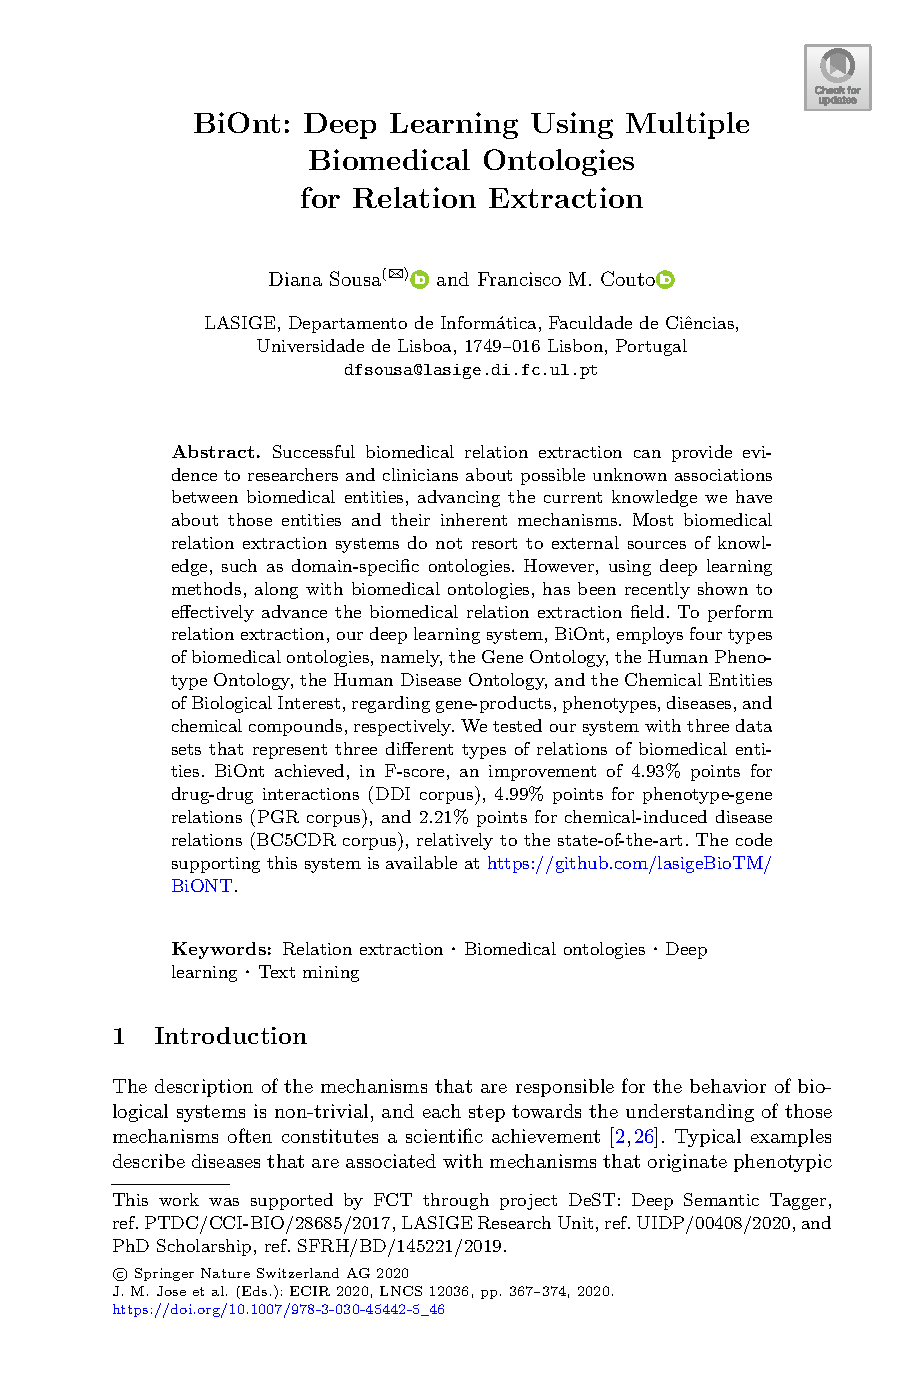
\includepdf[pages=-,scale=0.8]{articles/Sousa-Couto2020_Chapter_BiOntDeepLearningUsingMultiple.pdf}

\hypertarget{AC}{\chapter{Improving Accessibility and Distinction between Negative Results in Biomedical Relation Extraction}}
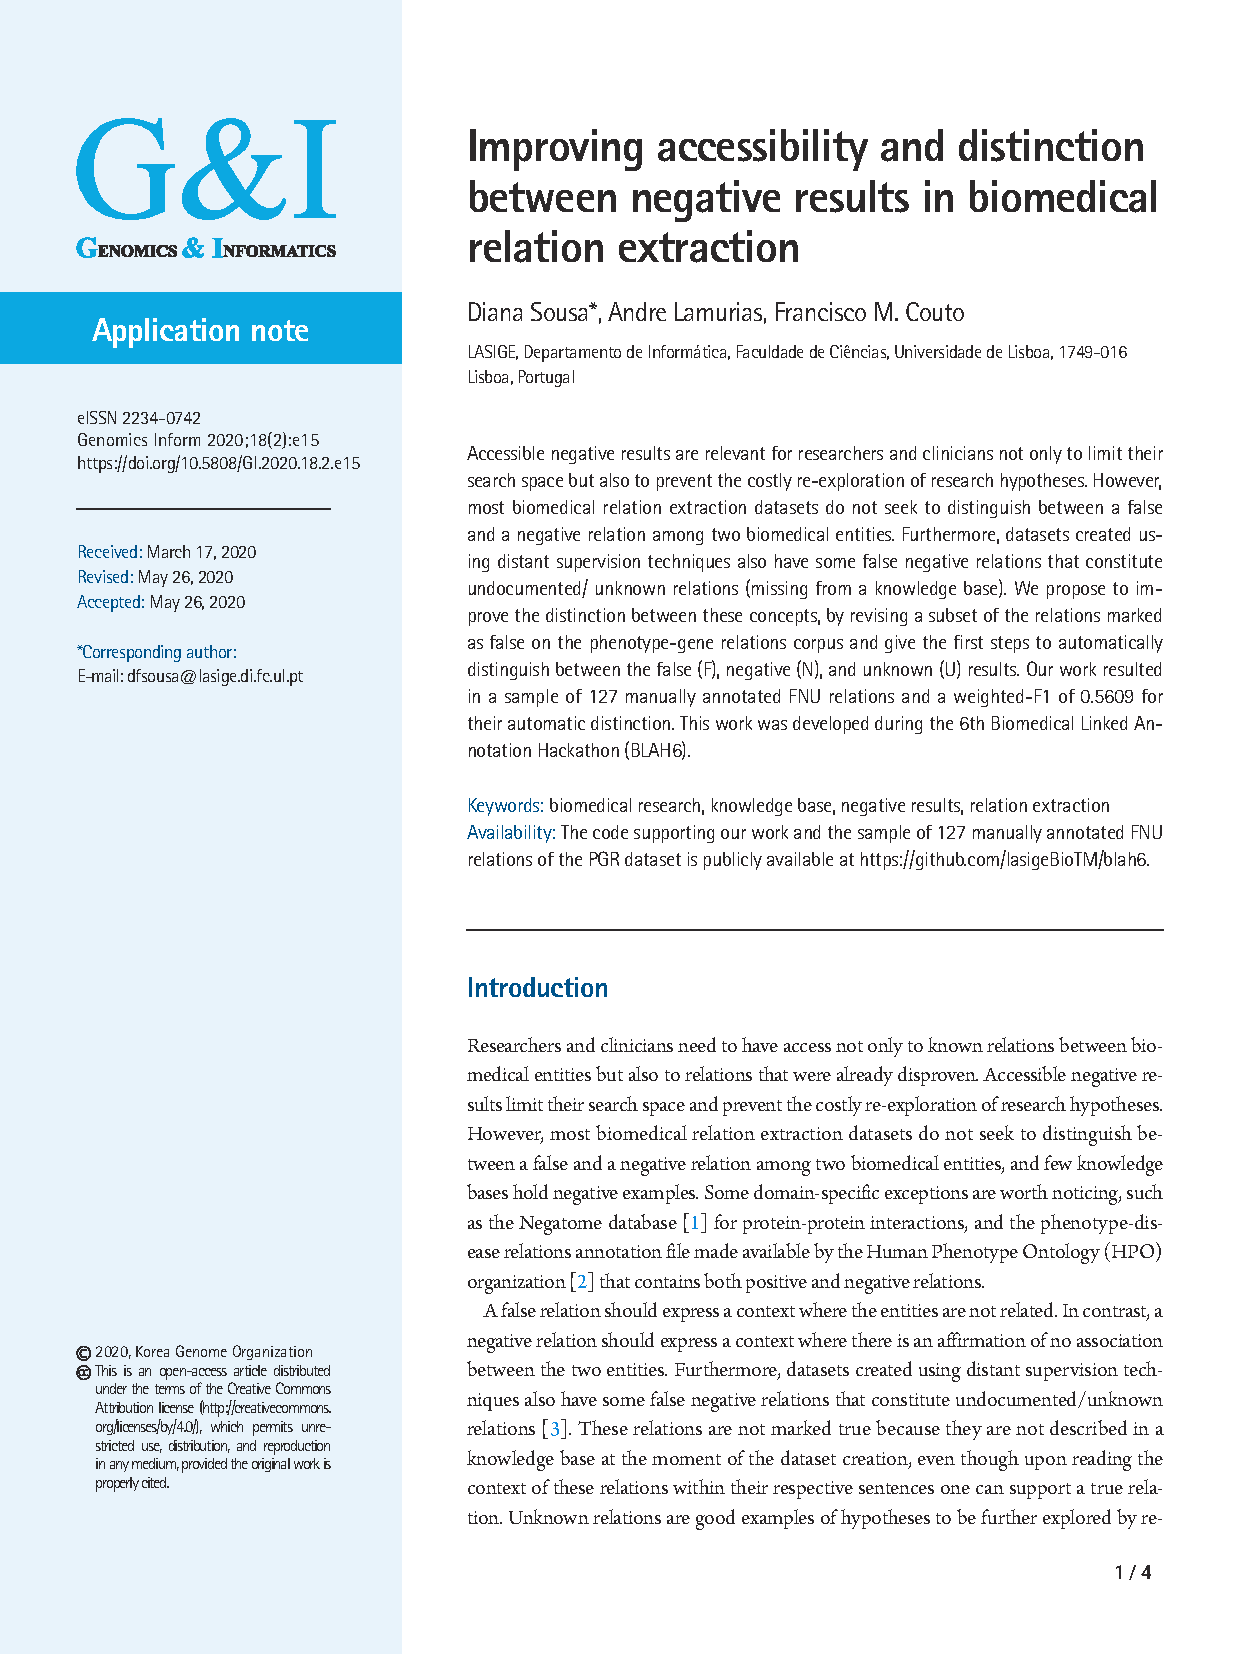
\includepdf[pages=-,scale=0.8]{articles/g_and_i.pdf}

\hypertarget{AD}{\chapter{A Hybrid Approach towards Biomedical Relation Extraction Training Corpora: Combining Distant Supervision with Crowdsourcing}}
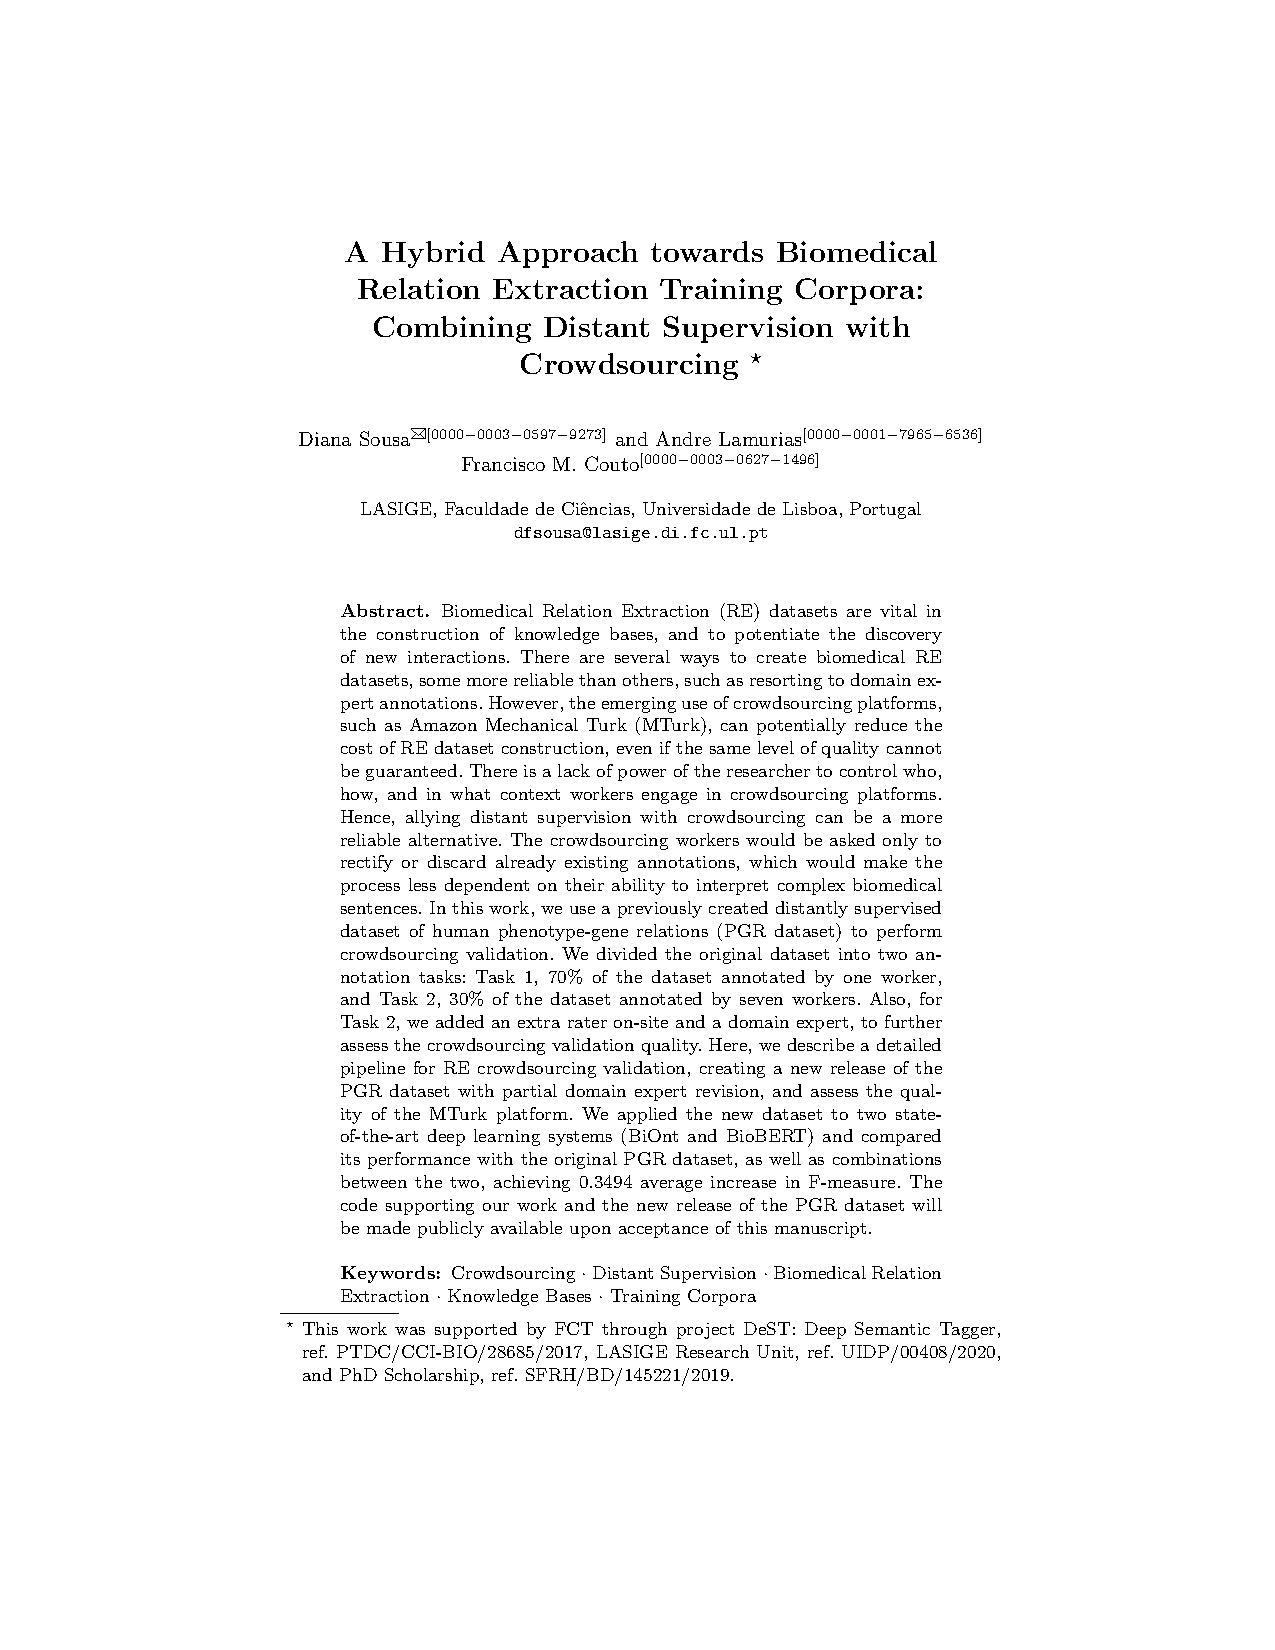
\includepdf[pages=-,scale=1]{articles/DATABASE_preprint.pdf}



\end{document}